%\subsection{Kinematic Observables} \label{sec:KinematicObservables}
\subsection{Extraction of differential H $\rightarrow 4\ell$ cross section} \label{sec:KinematicObservables}

\subsubsection{Considered observables} 
The
differential fiducial cross sections are presented as a function of several kinematic
observables which are sensitive to the Higgs-boson production mechanisms. Examples are rapidity and transverse momentum of the four-lepton system, associated jet multiplicity and transverse momentum of the leading jet $\pt({\rm H})$ or $\pt(4\ell)$, $|y({\rm H})|$ or $|y(4\ell)|$),$ N(jets)$, and $\pt({\rm jet})$. These measurements are
important to test the Standard Model predictions in the Higgs sector and can be
used to constrain phase spaces of many theories beyond the Standard Model.
%Measurements on differential cross section which are performed as function of the kinematic properties of four-lepton system and as well as  jet multiplicity are unfolded to the particle level.
In addition, several other observables related to decay of Higgs boson are also studied. These include $m_{Z_{1}}$, $m_{Z_{2}}$, $\phi$, $cos\theta^{*}$ and several other observables which are sensitive to spin and CP or Higgs bosons.  

\subsubsection{Choice of bin boundaries} 
For each kinematic or differential observable, selection procedure of the binning boundaries has been optimized in order to have a similar expected measured cross-section for every bin. Relative uncertainties for \pt of Higgs observables are given in Table. \ref{tab:resultspT4l}.

\begin{table}[!h!tb]
\begin{center}
\small
\caption{
Differential cross section results for the $p_{T}(H)$ observable.
\label{tab:resultspT4l}
}
\begin{tabular}{|c|ccccc|} \hline \hline
Bin range (GeV) & d$\sigma_{fid}$ (fb) & $\Delta_{tot}$ (\% fb) & $\Delta_{rel}$ (\%)  & $\delta_{stat}$ (\% fb)  & $\delta_{syst}$ (\% fb) \\ \hline \hline
\multicolumn{6}{|c|}{ \textbf{CMS preliminary choice }} \\ \hline
        0 - 10 &  0.34 &  $^{+0.11}_{-0.096}$ &  $^{+33}_{-28}$ &  $^{+0.1}_{-0.091}$ &  $^{+0.048}_{-0.031}$ \\ %0.32 &  $^{+11.01}_{-9.66}$ &  $^{+34.83}_{-30.55}$ &  $^{+10.20}_{-9.00}$ &  $^{+4.20}_{-3.40}$ \\
  10 - 20 &  0.53 &  $^{+0.13}_{-0.11}$ &  $^{+25}_{-21}$ &  $^{+0.12}_{-0.11}$ &  $^{+0.056}_{-0.037}$ \\ %0.67 &  $^{+13.98}_{-12.62}$ &  $^{+20.80}_{-18.78}$ &  $^{+12.70}_{-11.60}$ &  $^{+5.80}_{-4.90}$ \\
  20 - 30 &  0.42 &  $^{+0.11}_{-0.097}$ &  $^{+27}_{-23}$ &  $^{+0.1}_{-0.093}$ &  $^{+0.044}_{-0.027}$ \\ %0.41 &  $^{+11.77}_{-10.34}$ &  $^{+28.95}_{-25.43}$ &  $^{+10.90}_{-9.70}$ &  $^{+4.30}_{-3.50}$ \\
  30 - 45 &  0.43 &  $^{+0.11}_{-0.094}$ &  $^{+25}_{-22}$ &  $^{+0.1}_{-0.089}$ &  $^{+0.044}_{-0.029}$ \\ %0.51 &  $^{+11.72}_{-10.50}$ &  $^{+22.83}_{-20.45}$ &  $^{+10.80}_{-9.80}$ &  $^{+4.50}_{-3.80}$ \\
  45 - 80 &  0.52 &  $^{+0.11}_{-0.1}$ &  $^{+22}_{-19}$ &  $^{+0.1}_{-0.092}$ &  $^{+0.05}_{-0.038}$ \\ %0.45 &  $^{+10.46}_{-9.35}$ &  $^{+23.29}_{-20.82}$ &  $^{+9.80}_{-8.80}$ &  $^{+3.80}_{-3.20}$ \\
  80 - 120 &  0.25 &  $^{+0.073}_{-0.062}$ &  $^{+29}_{-25}$ &  $^{+0.069}_{-0.06}$ &  $^{+0.024}_{-0.018}$ \\ %0.30 &  $^{+7.72}_{-6.72}$ &  $^{+26.12}_{-22.75}$ &  $^{+7.40}_{-6.50}$ &  $^{+2.20}_{-1.80}$ \\
  120 - 200 &  0.18 &  $^{+0.057}_{-0.048}$ &  $^{+31}_{-26}$ &  $^{+0.055}_{-0.046}$ &  $^{+0.016}_{-0.011}$ \\ %0.19 &  $^{+5.74}_{-4.89}$ &  $^{+30.46}_{-25.91}$ &  $^{+5.60}_{-4.70}$ &  $^{+1.40}_{-1.20}$ \\
  200 - 13000 &  0.082 &  $^{+0.036}_{-0.028}$ &  $^{+44}_{-34}$ &  $^{+0.035}_{-0.028}$ &  $^{+0.008}_{-0.004}$ \\ %0.03 &  $^{+2.20}_{-1.50}$ &  $^{+80.48}_{-54.92}$ &  $^{+2.20}_{-1.50}$ &  $^{+0.20}_{-0.10}$ \\

\hline
Total bins = 8 &$\sigma_{fid} = \Sigma d\sigma_{fid}$ = 2.8 (fb) & & & & &
        \hline






%\begin{tabular}{|c|ccccc|} \hline \hline
%Bin range (GeV) & d$\sigma$ (fb) & $\epsilon$ & $\epsilon_{rel}$ & $\epsilon_{stat}$  & $\epsilon_{syst}$ \\ \hline \hline
% 0 - 10 &  0.405 &  $^{+0.176}_{-0.139}$ &  $^{+0.435}_{-0.344}$ &  $^{+0.167}_{-0.142}$ &  $^{+0.054}_{-0.000}$ \\
%  10 - 20 &  0.535 &  $^{+0.186}_{-0.157}$ &  $^{+0.347}_{-0.294}$ &  $^{+0.177}_{-0.149}$ &  $^{+0.055}_{-0.051}$ \\
%  20 - 30 &  0.319 &  $^{+0.164}_{-0.132}$ &  $^{+0.512}_{-0.414}$ &  $^{+0.156}_{-0.128}$ &  $^{+0.050}_{-0.033}$ \\
%  30 - 45 &  0.447 &  $^{+0.163}_{-0.135}$ &  $^{+0.364}_{-0.302}$ &  $^{+0.155}_{-0.132}$ &  $^{+0.049}_{-0.028}$ \\
%  45 - 60 &  0.363 &  $^{+0.144}_{-0.119}$ &  $^{+0.396}_{-0.326}$ &  $^{+0.137}_{-0.115}$ &  $^{+0.043}_{-0.031}$ \\
%  60 - 80 &  0.079 &  $^{+0.073}_{-0.053}$ &  $^{+0.923}_{-0.674}$ &  $^{+0.072}_{-0.053}$ &  $^{+0.011}_{-0.007}$ \\
%  80 - 120 &  0.416 &  $^{+0.131}_{-0.108}$ &  $^{+0.316}_{-0.260}$ &  $^{+0.124}_{-0.108}$ &  $^{+0.044}_{-0.000}$ \\
%  120 - 200 &  0.112 &  $^{+0.074}_{-0.055}$ &  $^{+0.665}_{-0.489}$ &  $^{+0.000}_{-0.112}$ &  $^{+0.074}_{-0.000}$ \\
%  200 - 350 &  0.019 &  $^{+0.000}_{-0.019}$ &  $^{+0.000}_{-1.000}$ &  $^{+0.029}_{-0.019}$ &  $^{+0.000}_{-0.000}$ \\
%  350 - 1000 &  0.000 &  $^{+0.015}_{-0.000}$ &  $^{+14700.000}_{-0.000}$ &  $^{+0.015}_{-0.000}$ &  $^{+0.001}_{-0.000}$ \\
%
%\hline
%        Sum of individual bins' cross section ($\sigma$) & 2.695 (fb) & & & & &
%\hline
\hline
\end{tabular}
\normalsize
\end{center}
\end{table}


%%%%%%%%%%%%%%
%%\begin{figure}[!ht]
%%  \begin{center}
%%
%%    \subfigure[$0.0 < \pt(4\ell) < 15.0$]{
%%      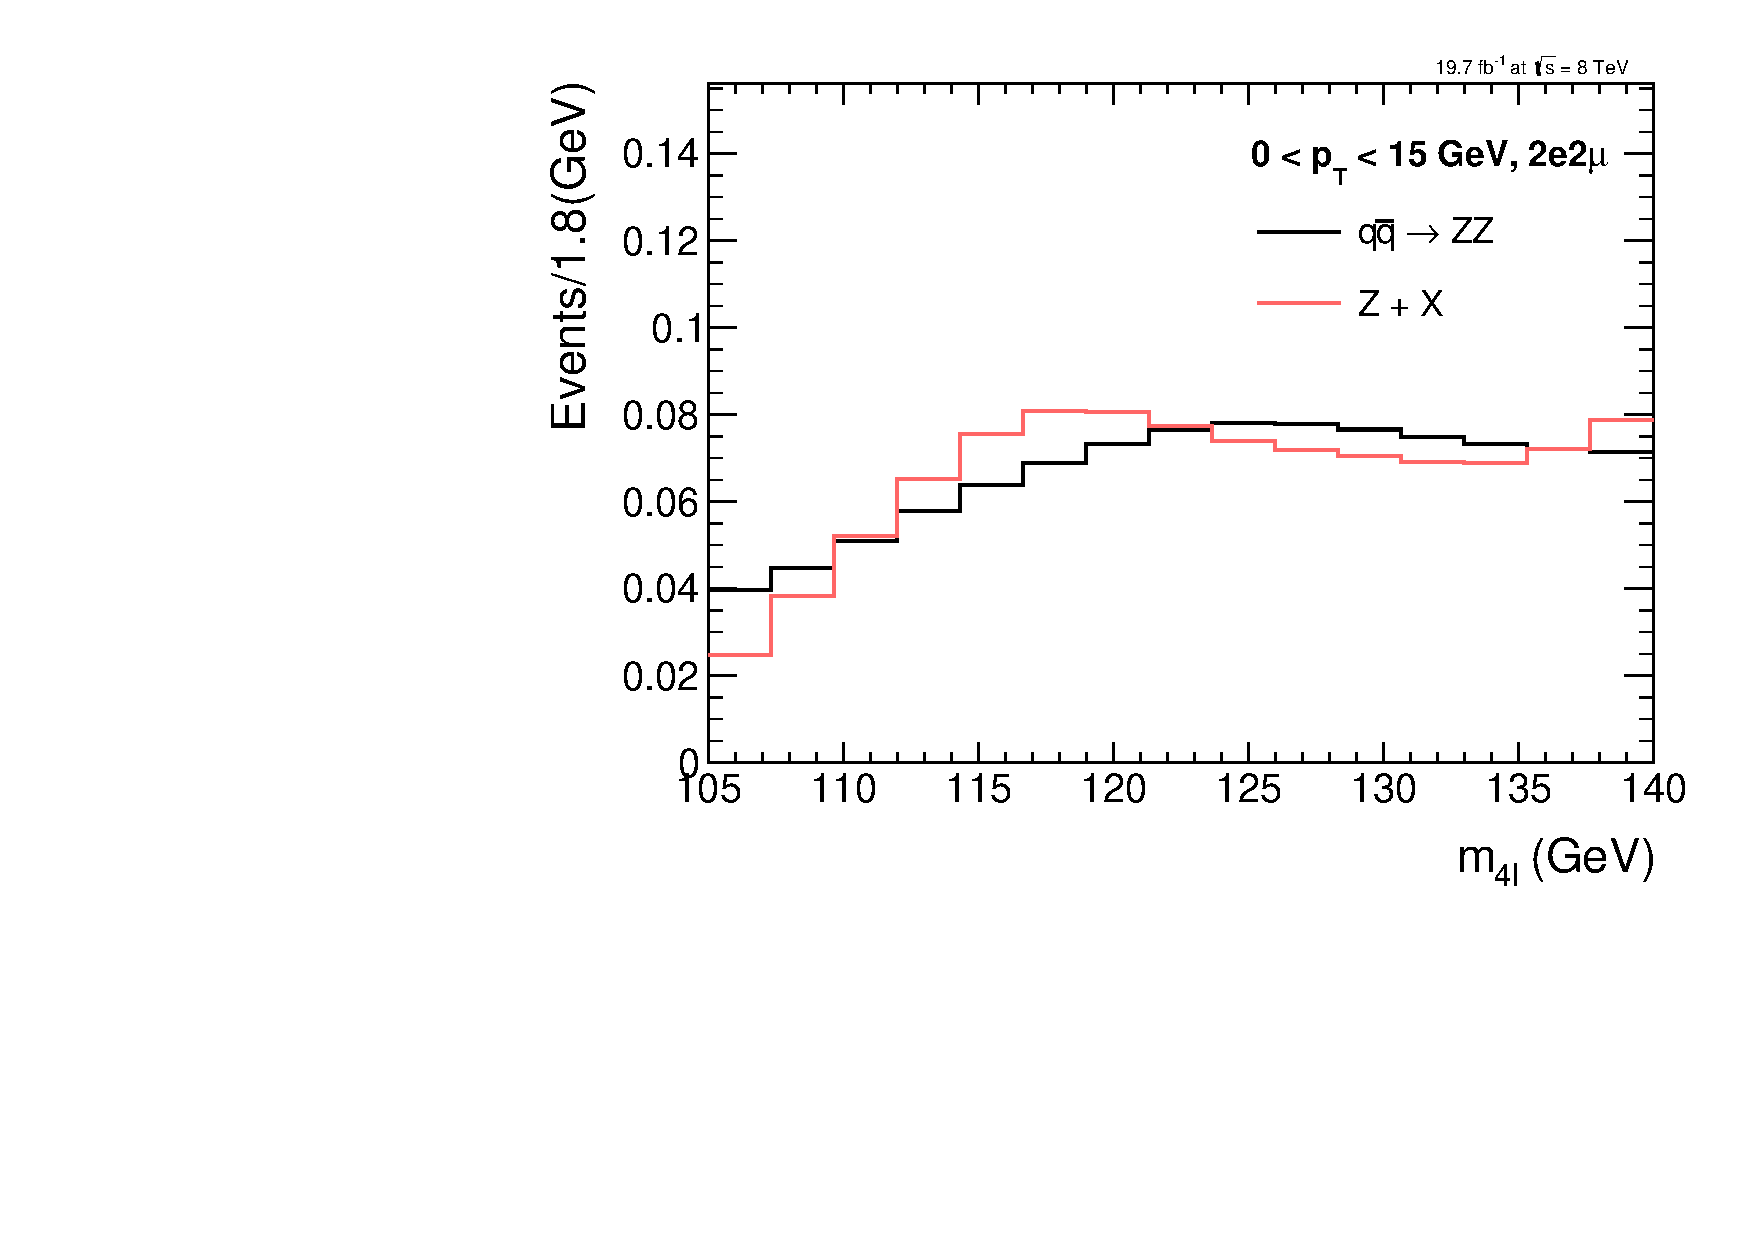
\includegraphics[width=0.3\textwidth,angle=0]{Appendix/figures/XSTemplates_2e2mu_pT4l_0_15_qqZZ_ZJetsCR.pdf}
%%    }
%%    \subfigure[$0.0< \pt(4\ell) < 15.0$]{
%%      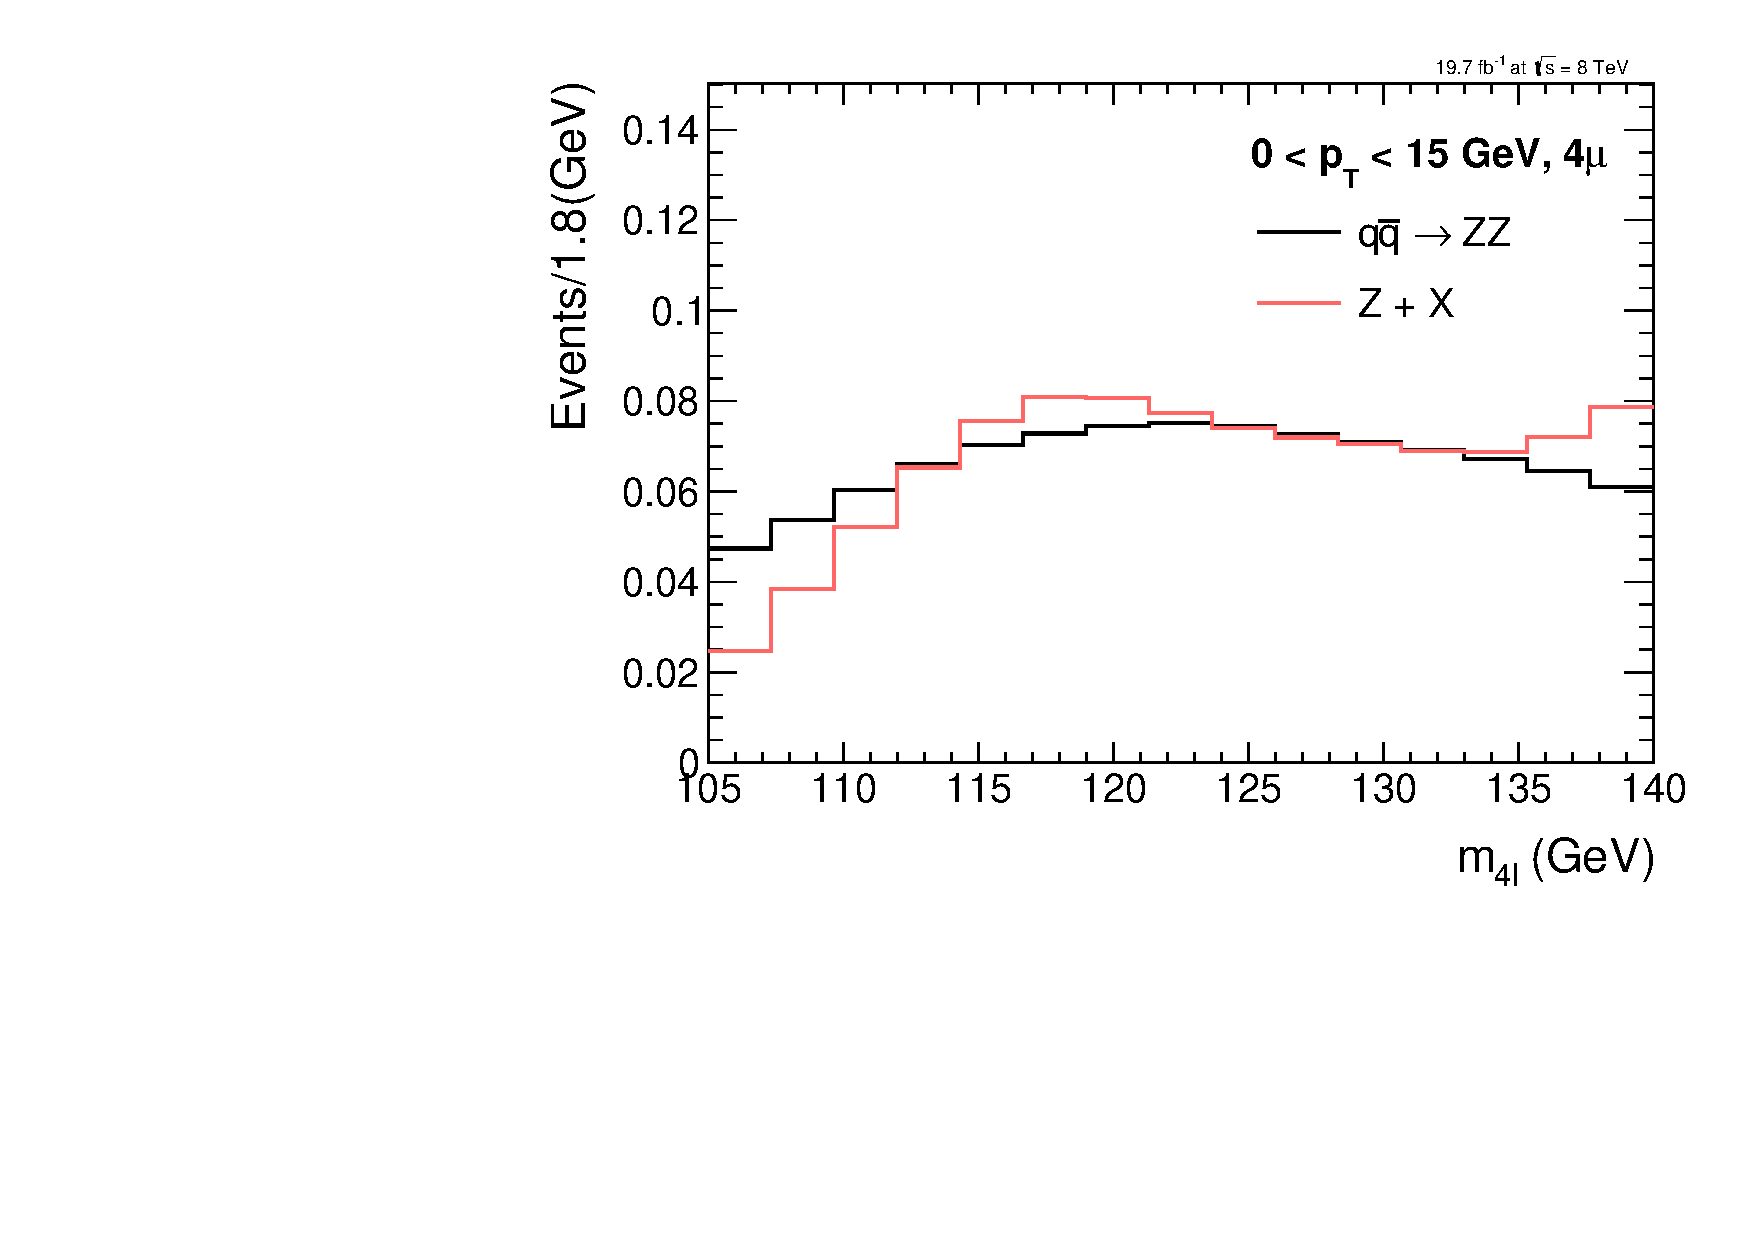
\includegraphics[width=0.3\textwidth,angle=0]{Appendix/figures/XSTemplates_4mu_pT4l_0_15_qqZZ_ZJetsCR.pdf}
%%    }
%%    \subfigure[$0.0 < \pt(4\ell) < 15.0$]{
%%      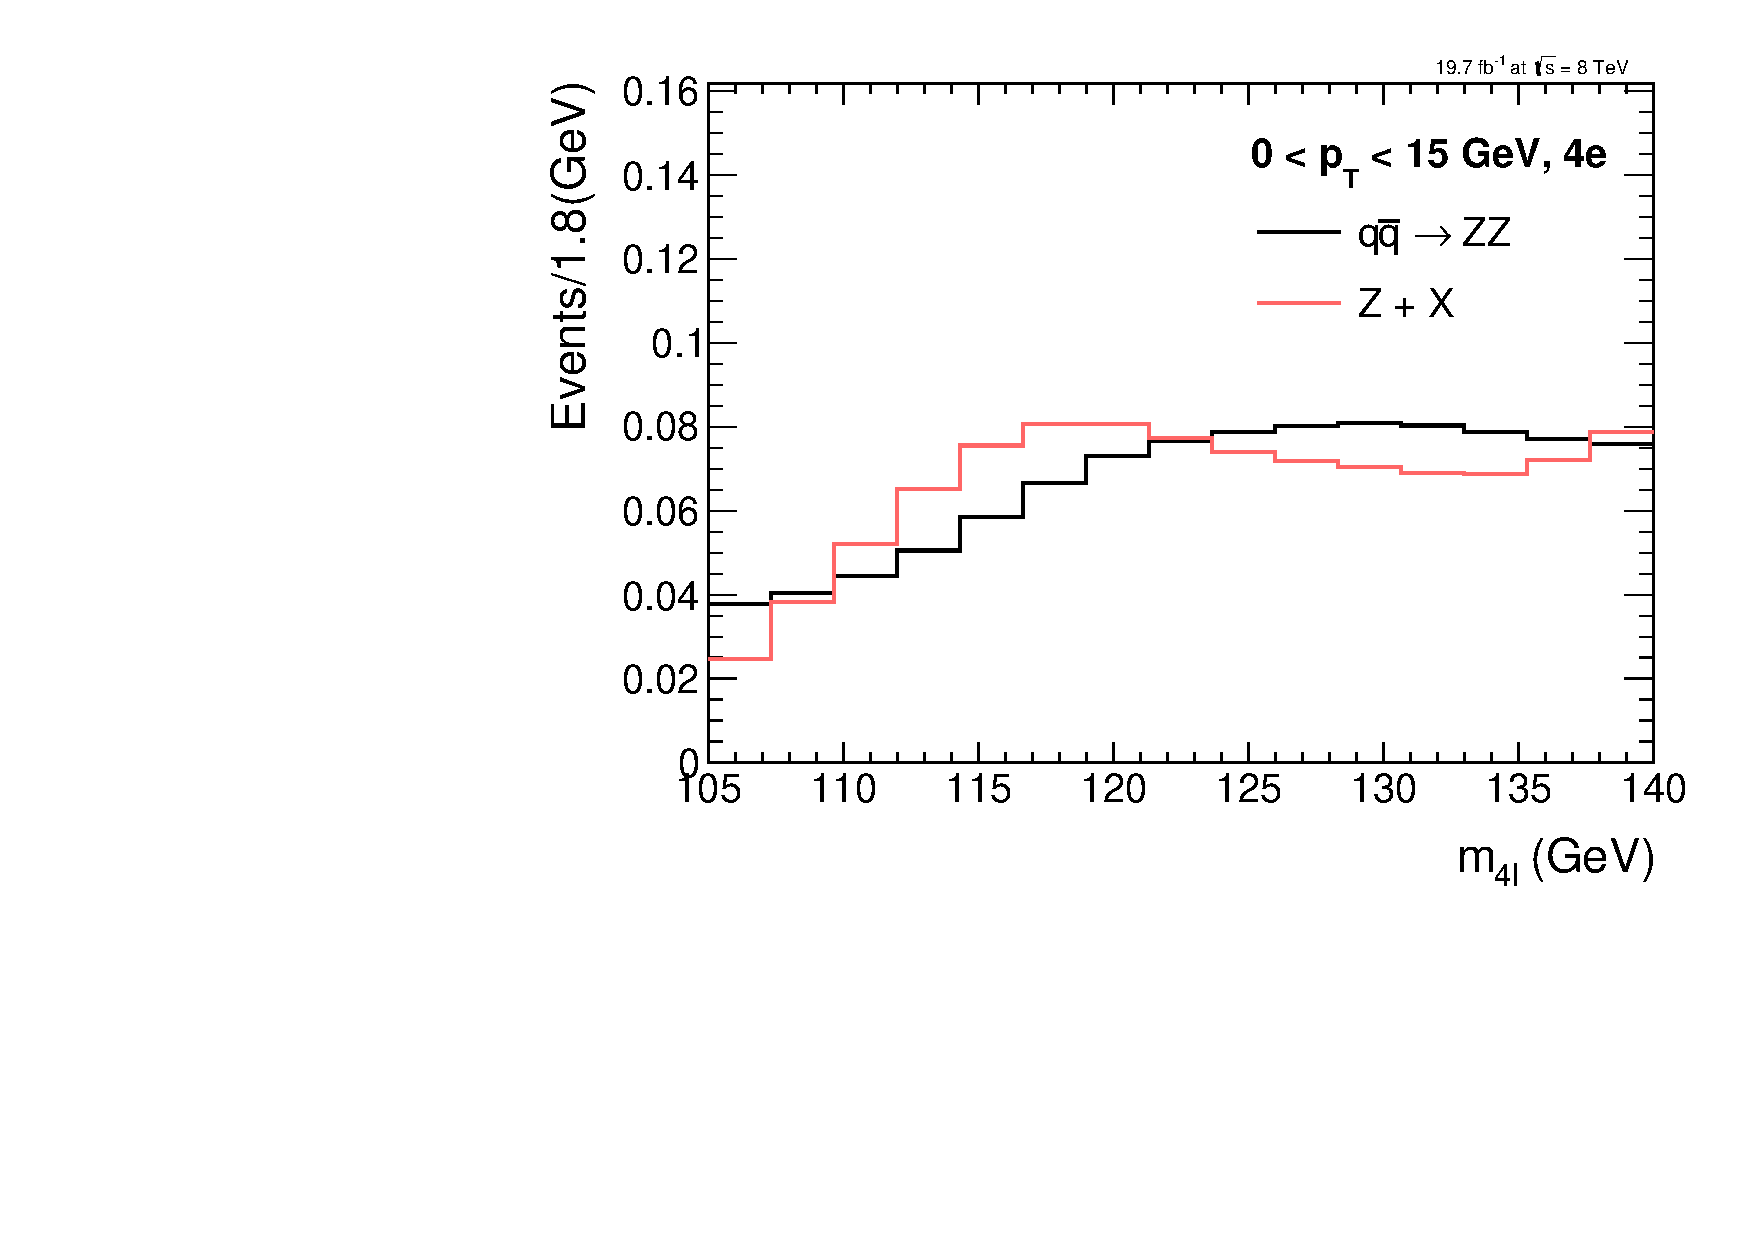
\includegraphics[width=0.3\textwidth,angle=0]{Appendix/figures/XSTemplates_4e_pT4l_0_15_qqZZ_ZJetsCR.pdf}
%%    }    \\
%% 
%%    \subfigure[$15.0 < \pt(4\ell) < 30.0$]{
%%      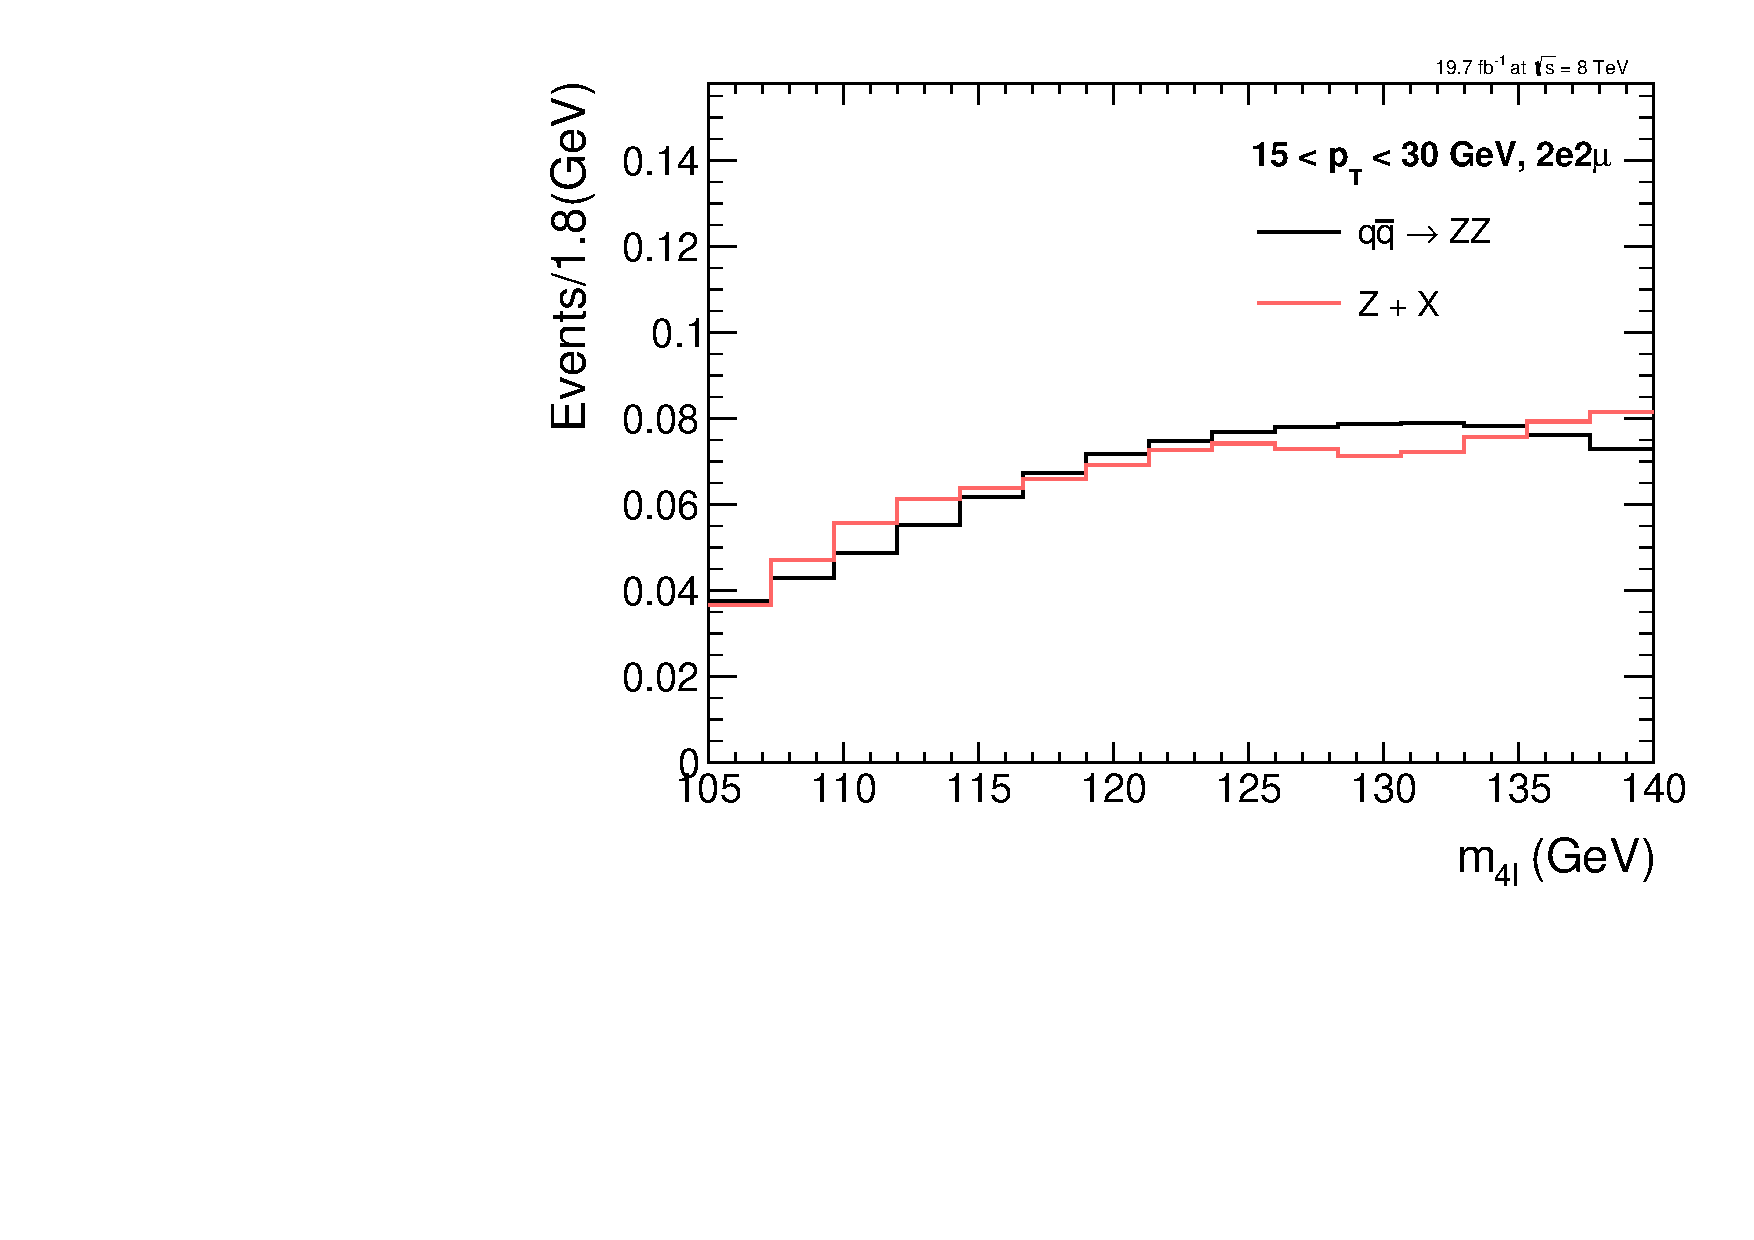
\includegraphics[width=0.3\textwidth,angle=0]{Appendix/figures/XSTemplates_2e2mu_pT4l_15_30_qqZZ_ZJetsCR.pdf}
%%    }
%%    \subfigure[$15.0 < \pt(4\ell) < 30.0$]{
%%      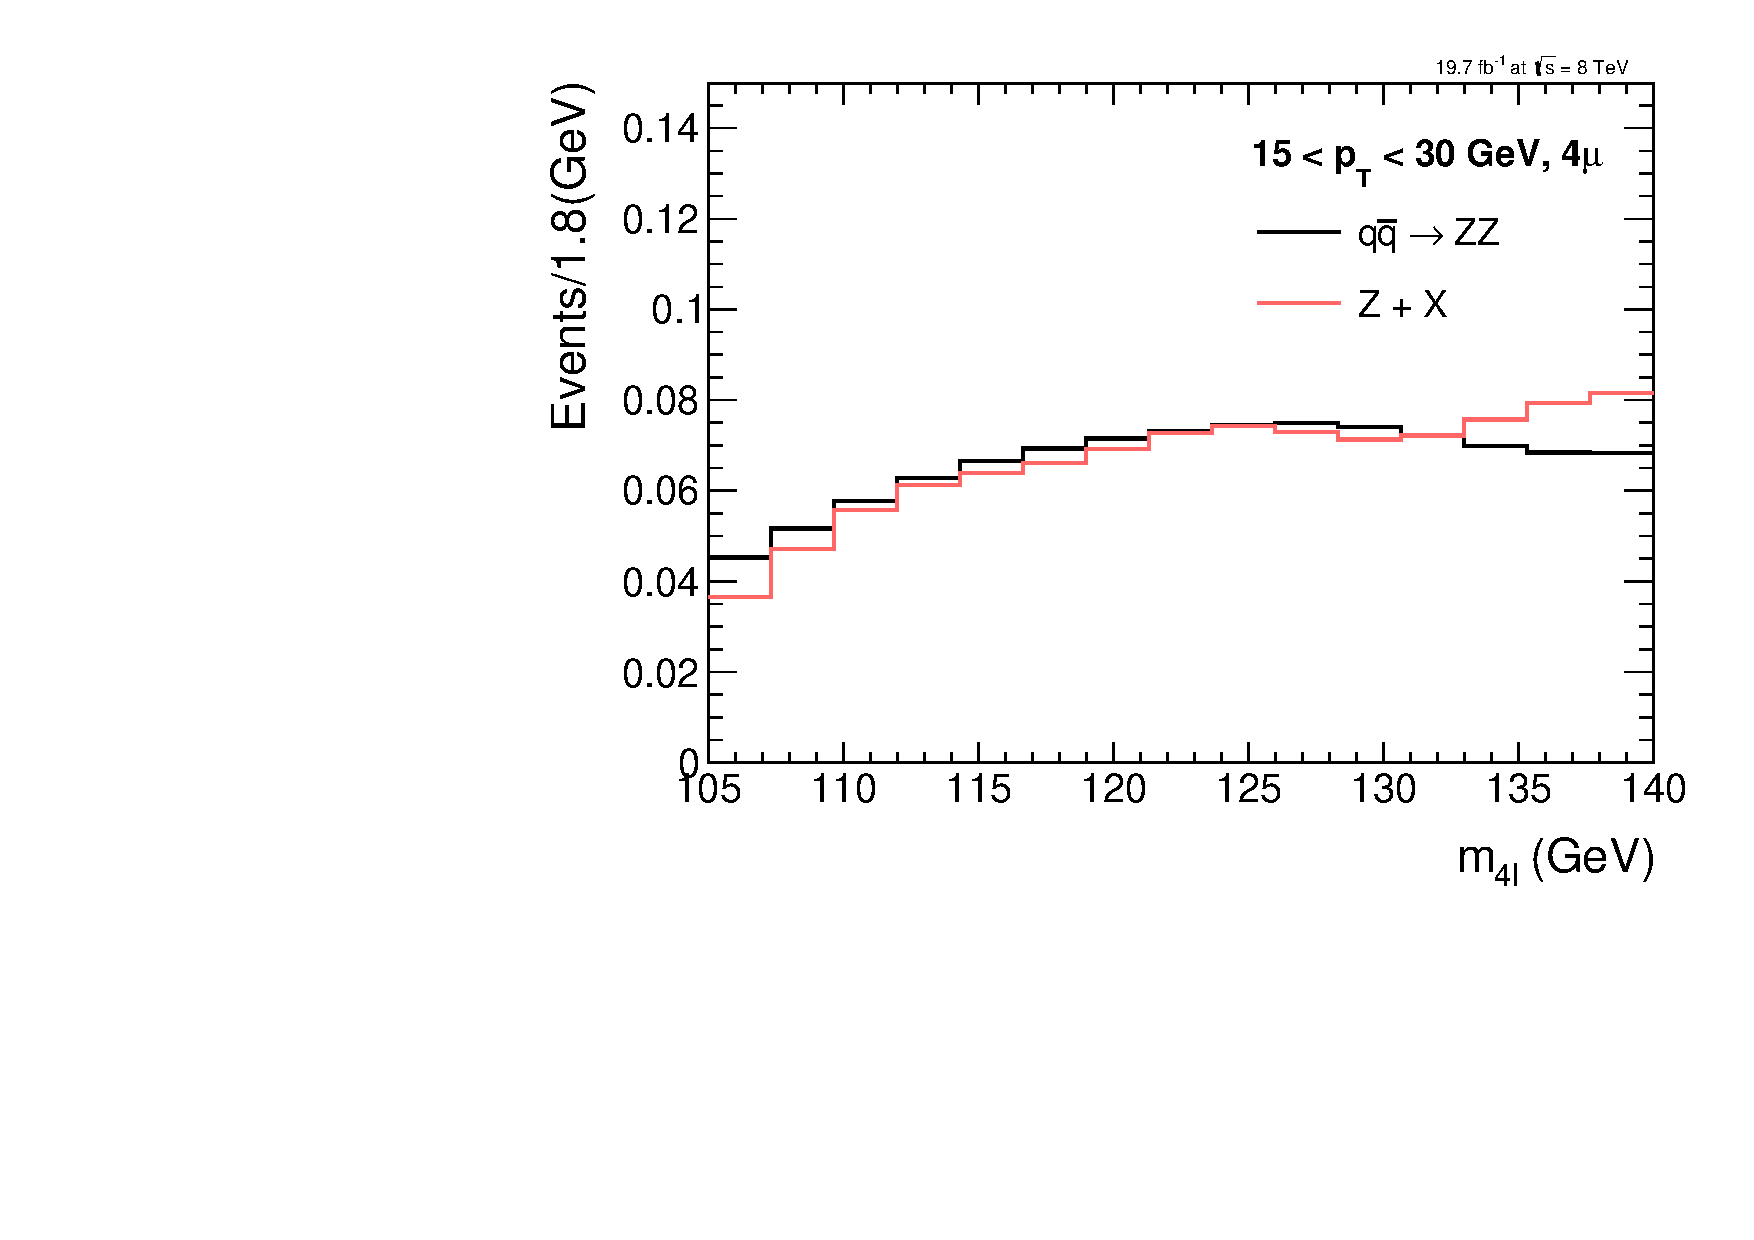
\includegraphics[width=0.3\textwidth,angle=0]{Appendix/figures/XSTemplates_4mu_pT4l_15_30_qqZZ_ZJetsCR.pdf}
%%    }
%%    \subfigure[$15.0  < \pt(4\ell) < 30.0$]{
%%      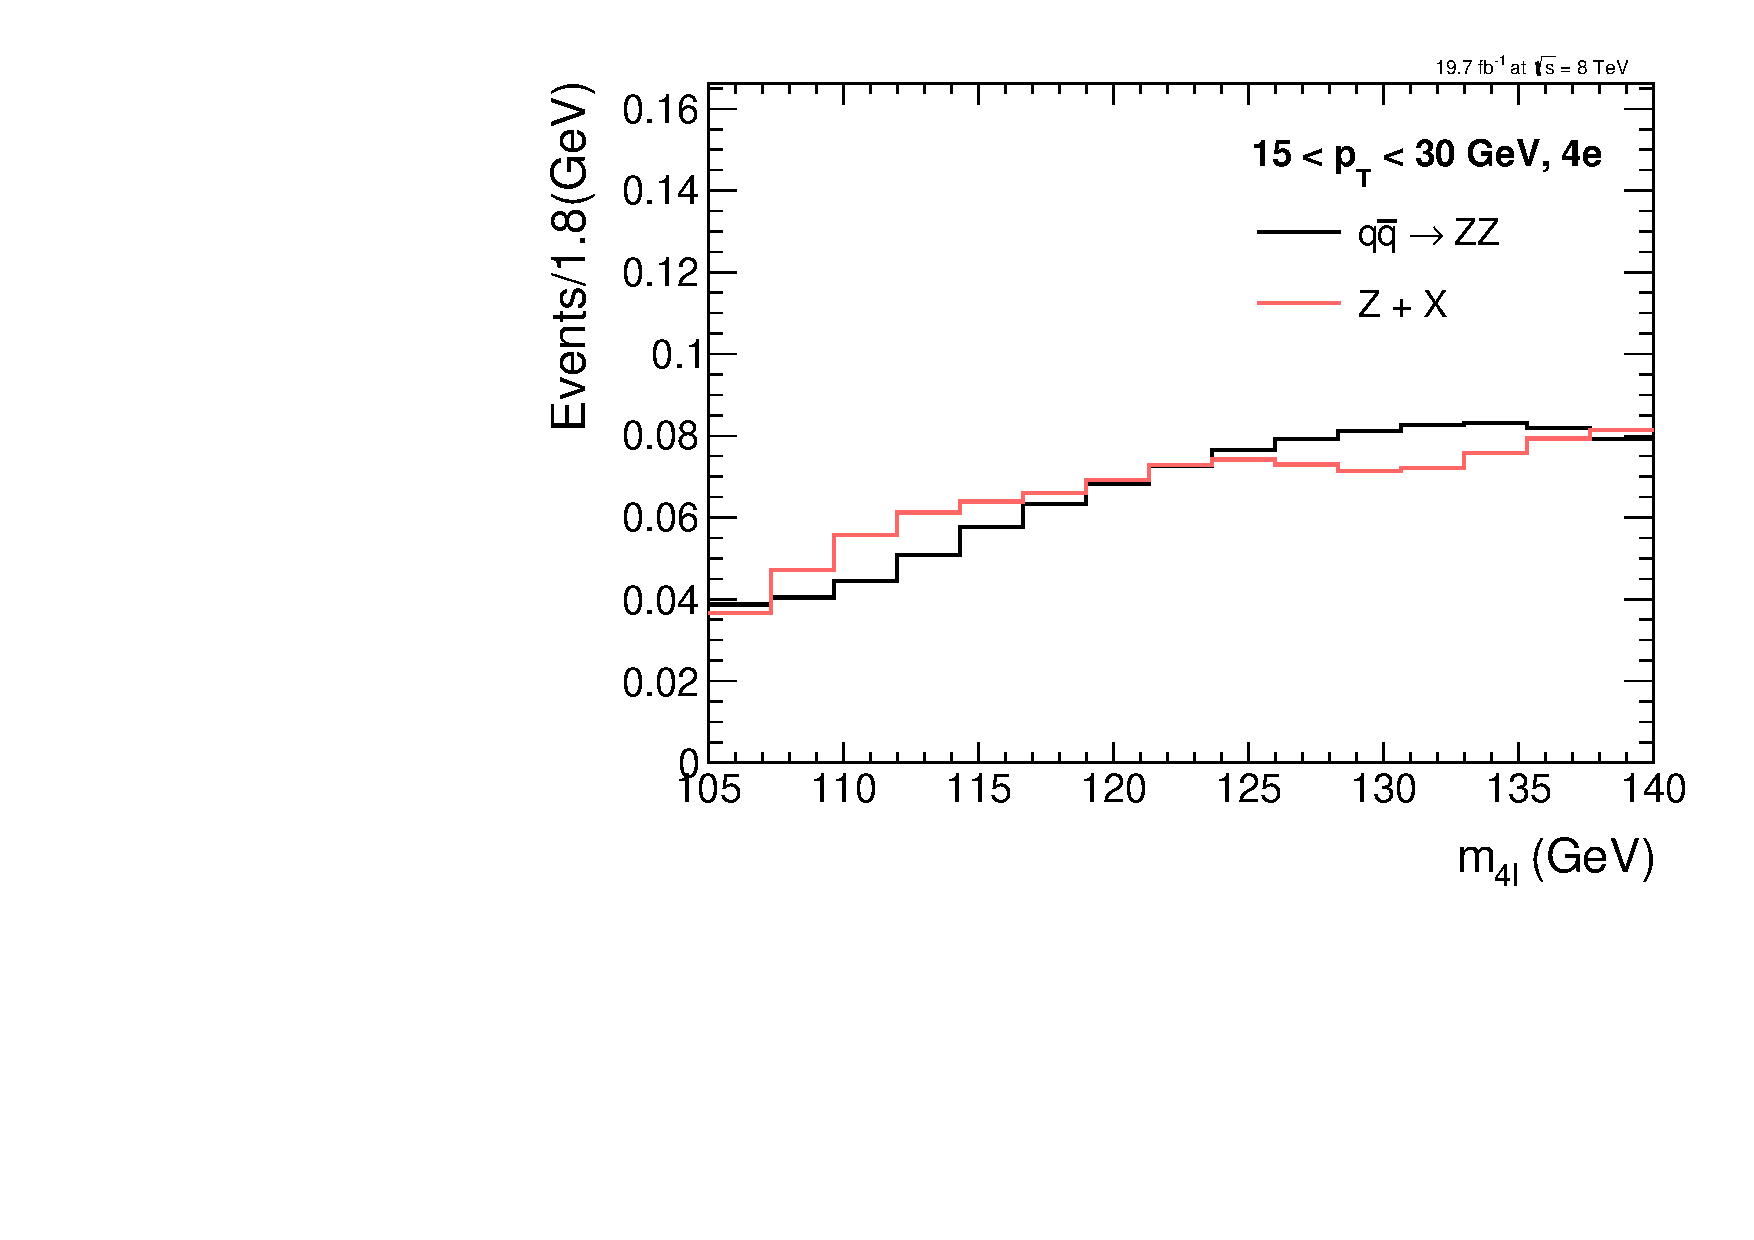
\includegraphics[width=0.3\textwidth,angle=0]{Appendix/figures/XSTemplates_4e_pT4l_15_30_qqZZ_ZJetsCR.pdf}
%%    } \\
%% 
%%    \subfigure[$30.0 < \pt(4\ell) < 60.0$ ]{
%%      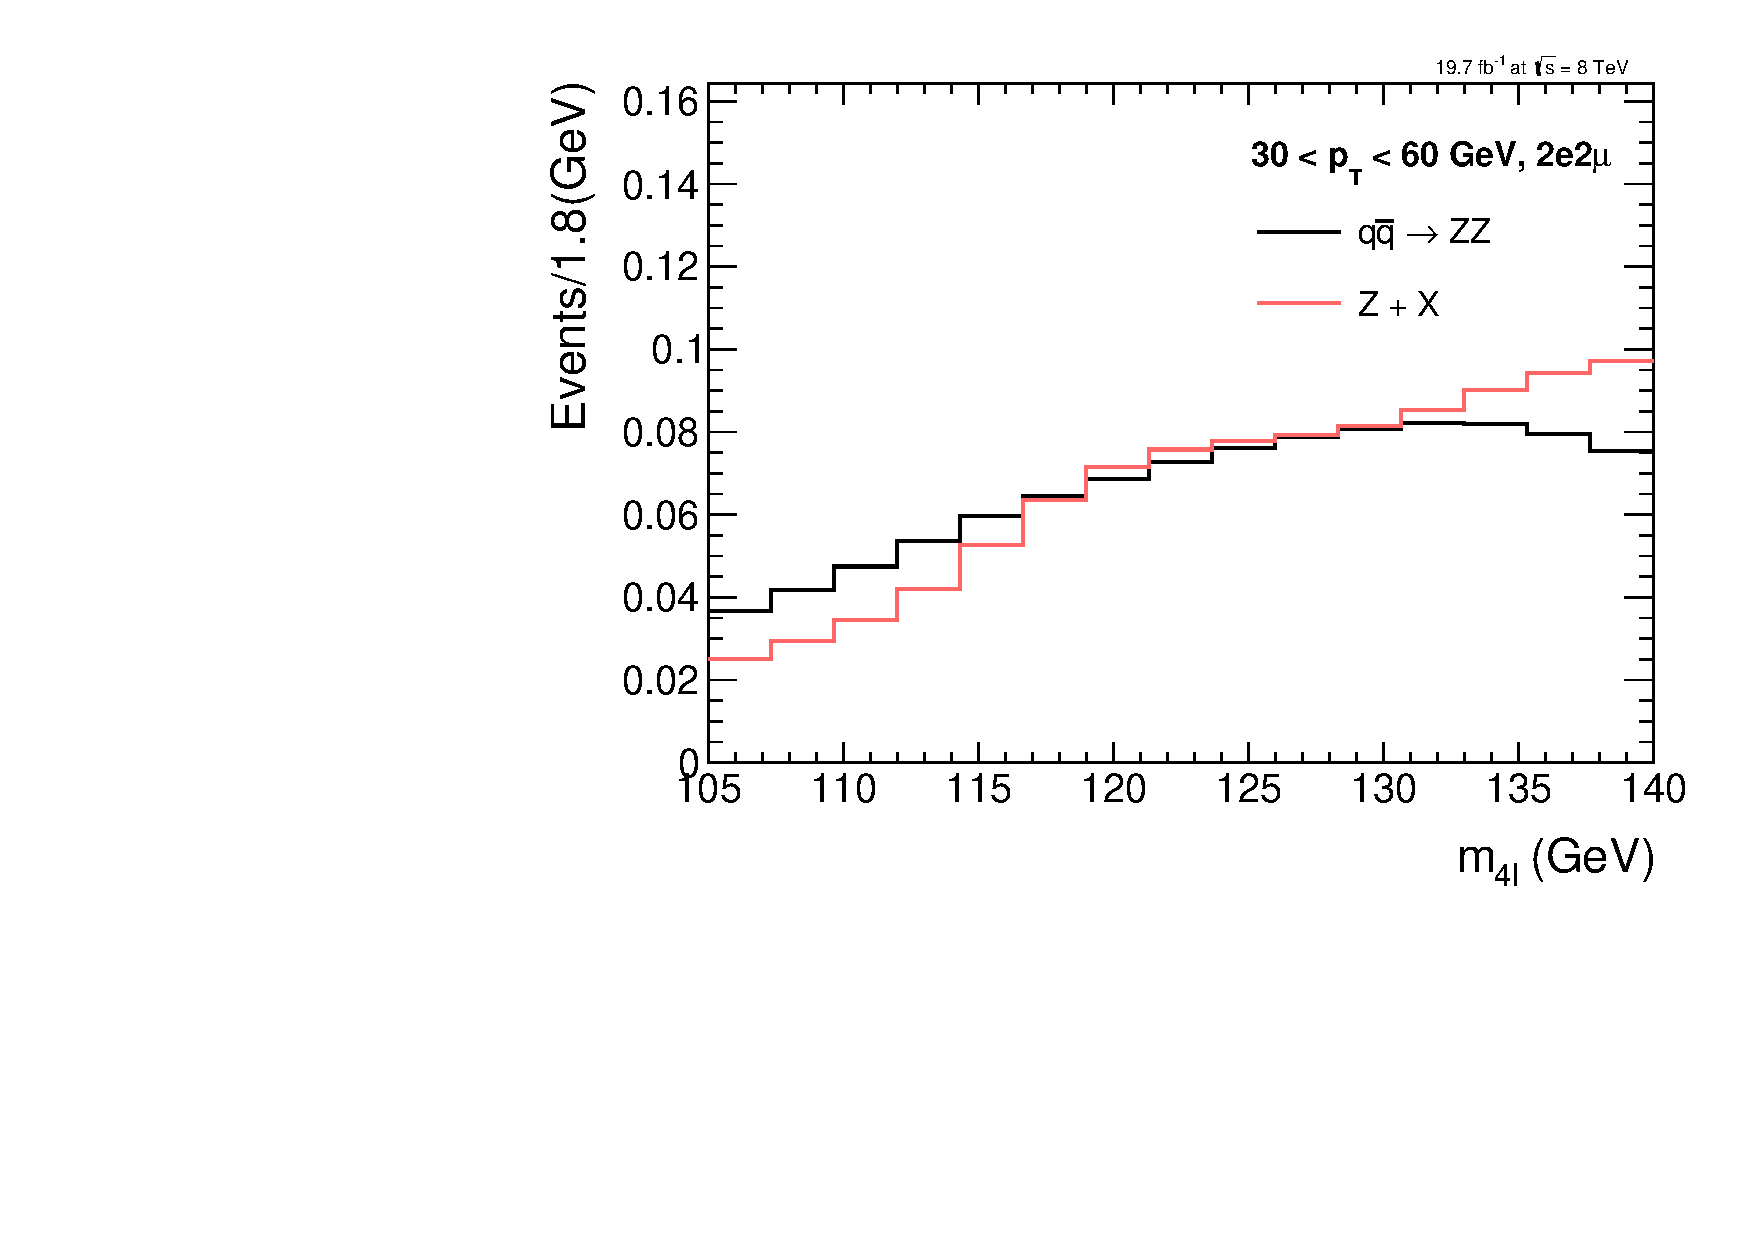
\includegraphics[width=0.3\textwidth,angle=0]{Appendix/figures/XSTemplates_2e2mu_pT4l_30_60_qqZZ_ZJetsCR.pdf}
%%    }
%%    \subfigure[$30.0 < \pt(4\ell) < 60.0$]{
%%      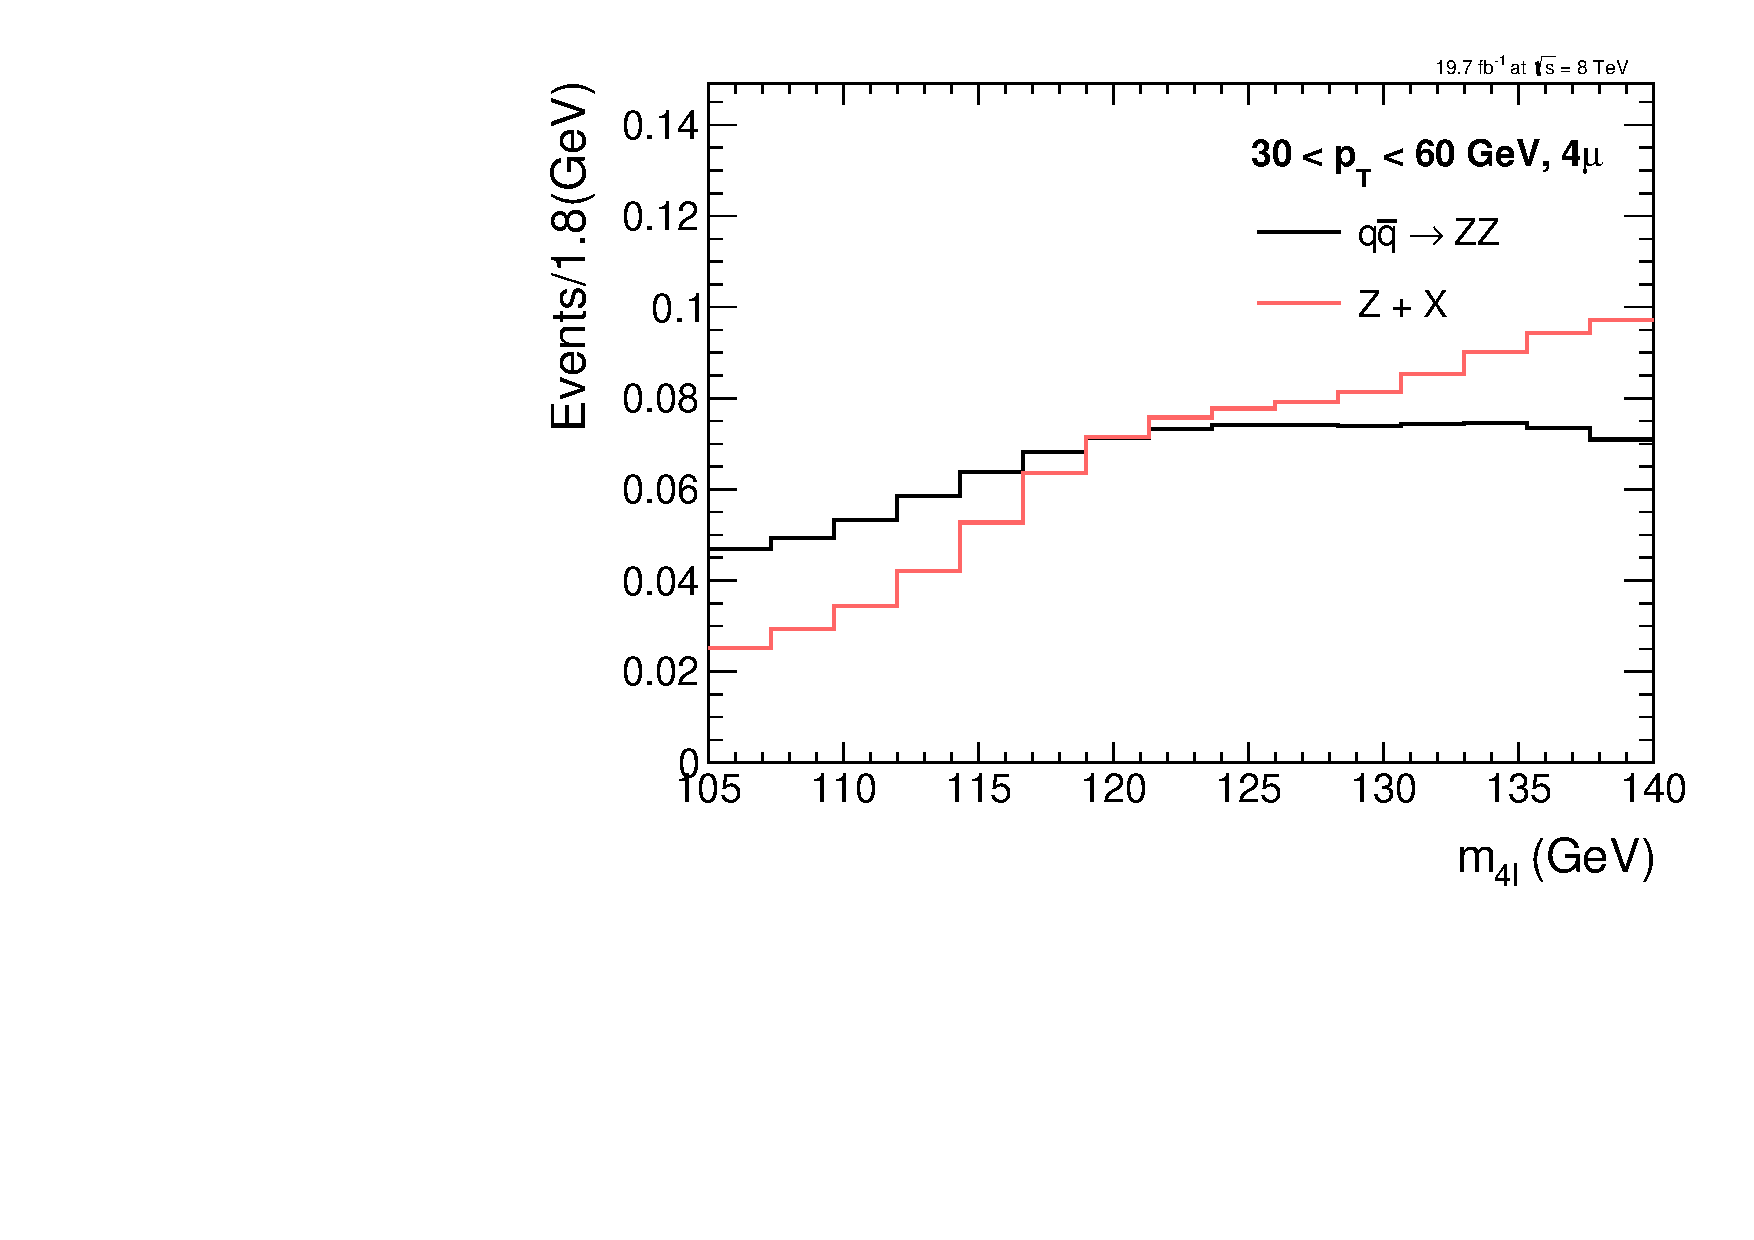
\includegraphics[width=0.3\textwidth,angle=0]{Appendix/figures/XSTemplates_4mu_pT4l_30_60_qqZZ_ZJetsCR.pdf}
%%    }
%%    \subfigure[$30.0 < \pt(4\ell) < 60.0$]{
%%      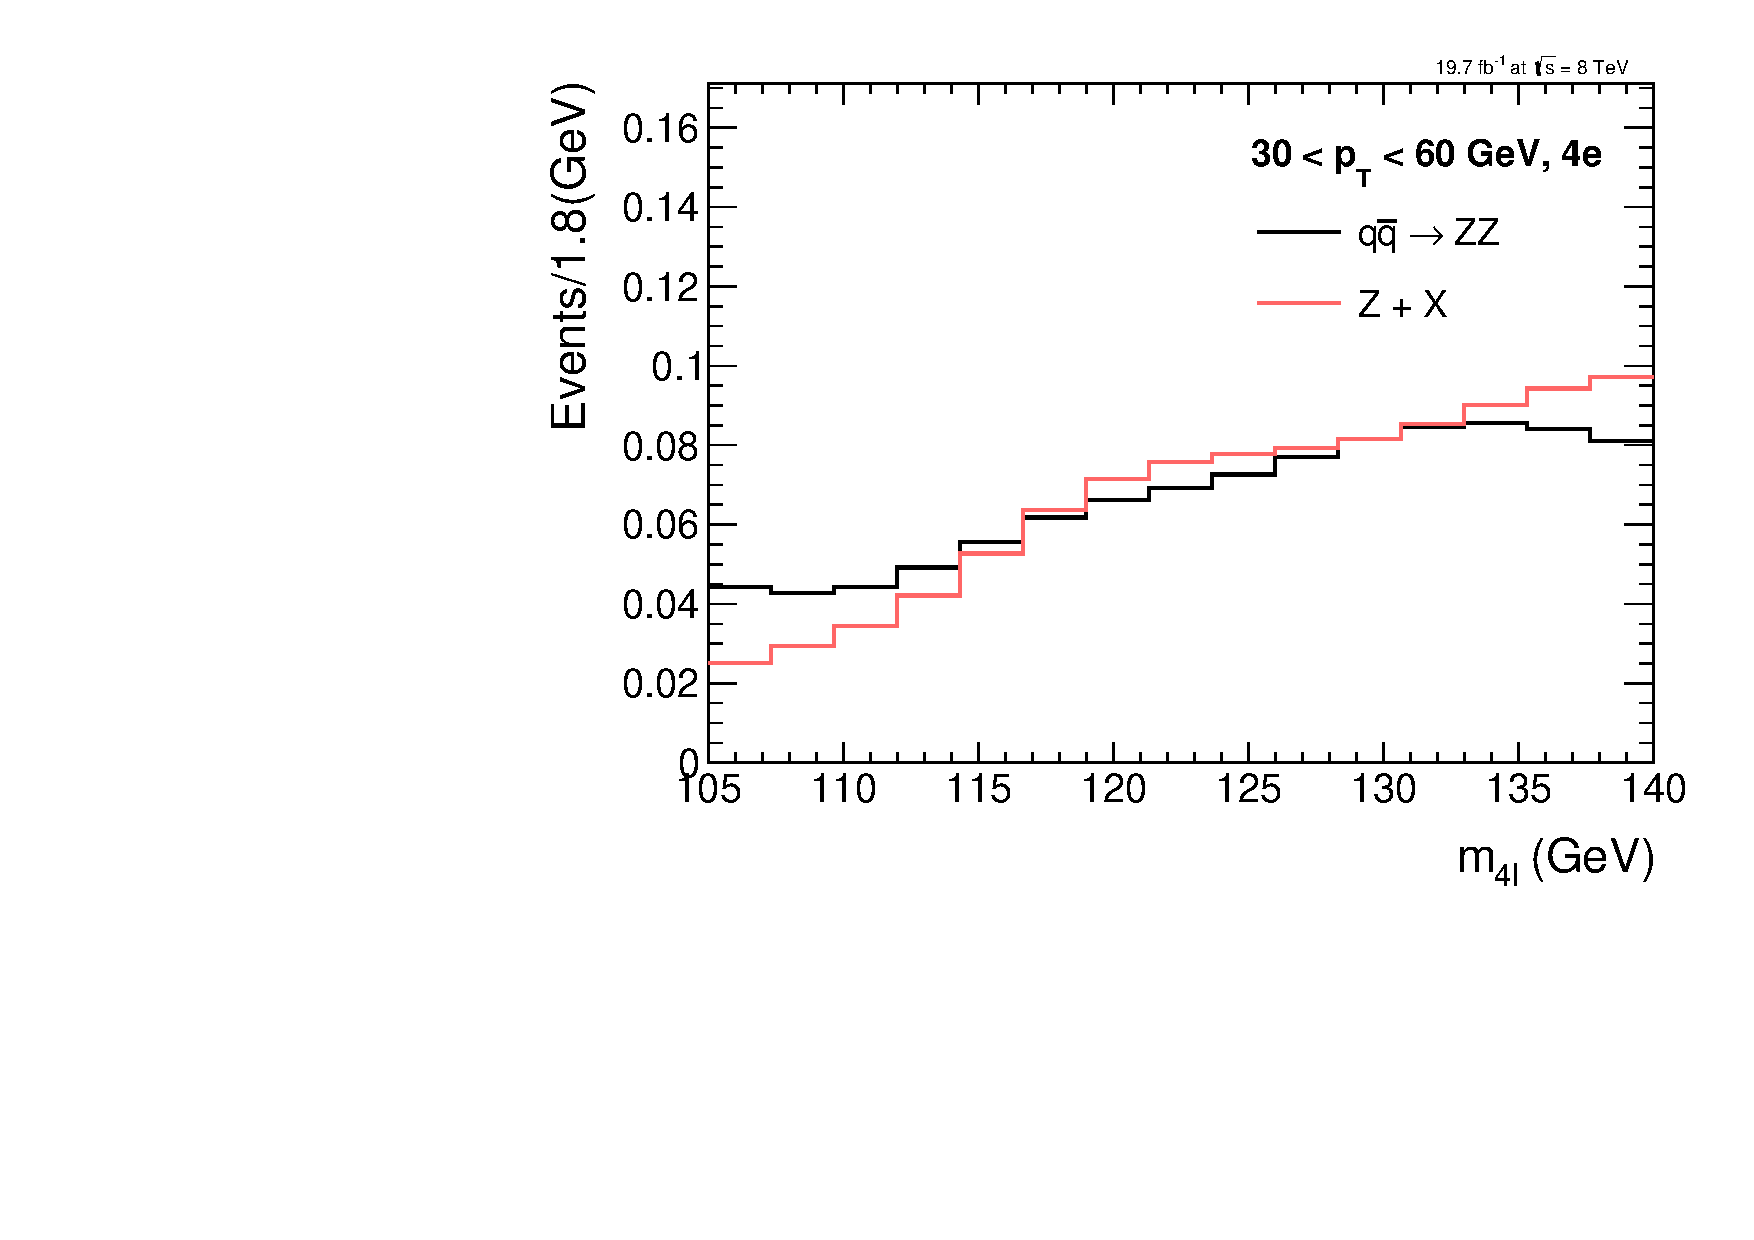
\includegraphics[width=0.3\textwidth,angle=0]{Appendix/figures/XSTemplates_4e_pT4l_30_60_qqZZ_ZJetsCR.pdf}
%%    } \\
%%
%%    \subfigure[$60.0 < \pt(4\ell) < 200.0$]{
%%      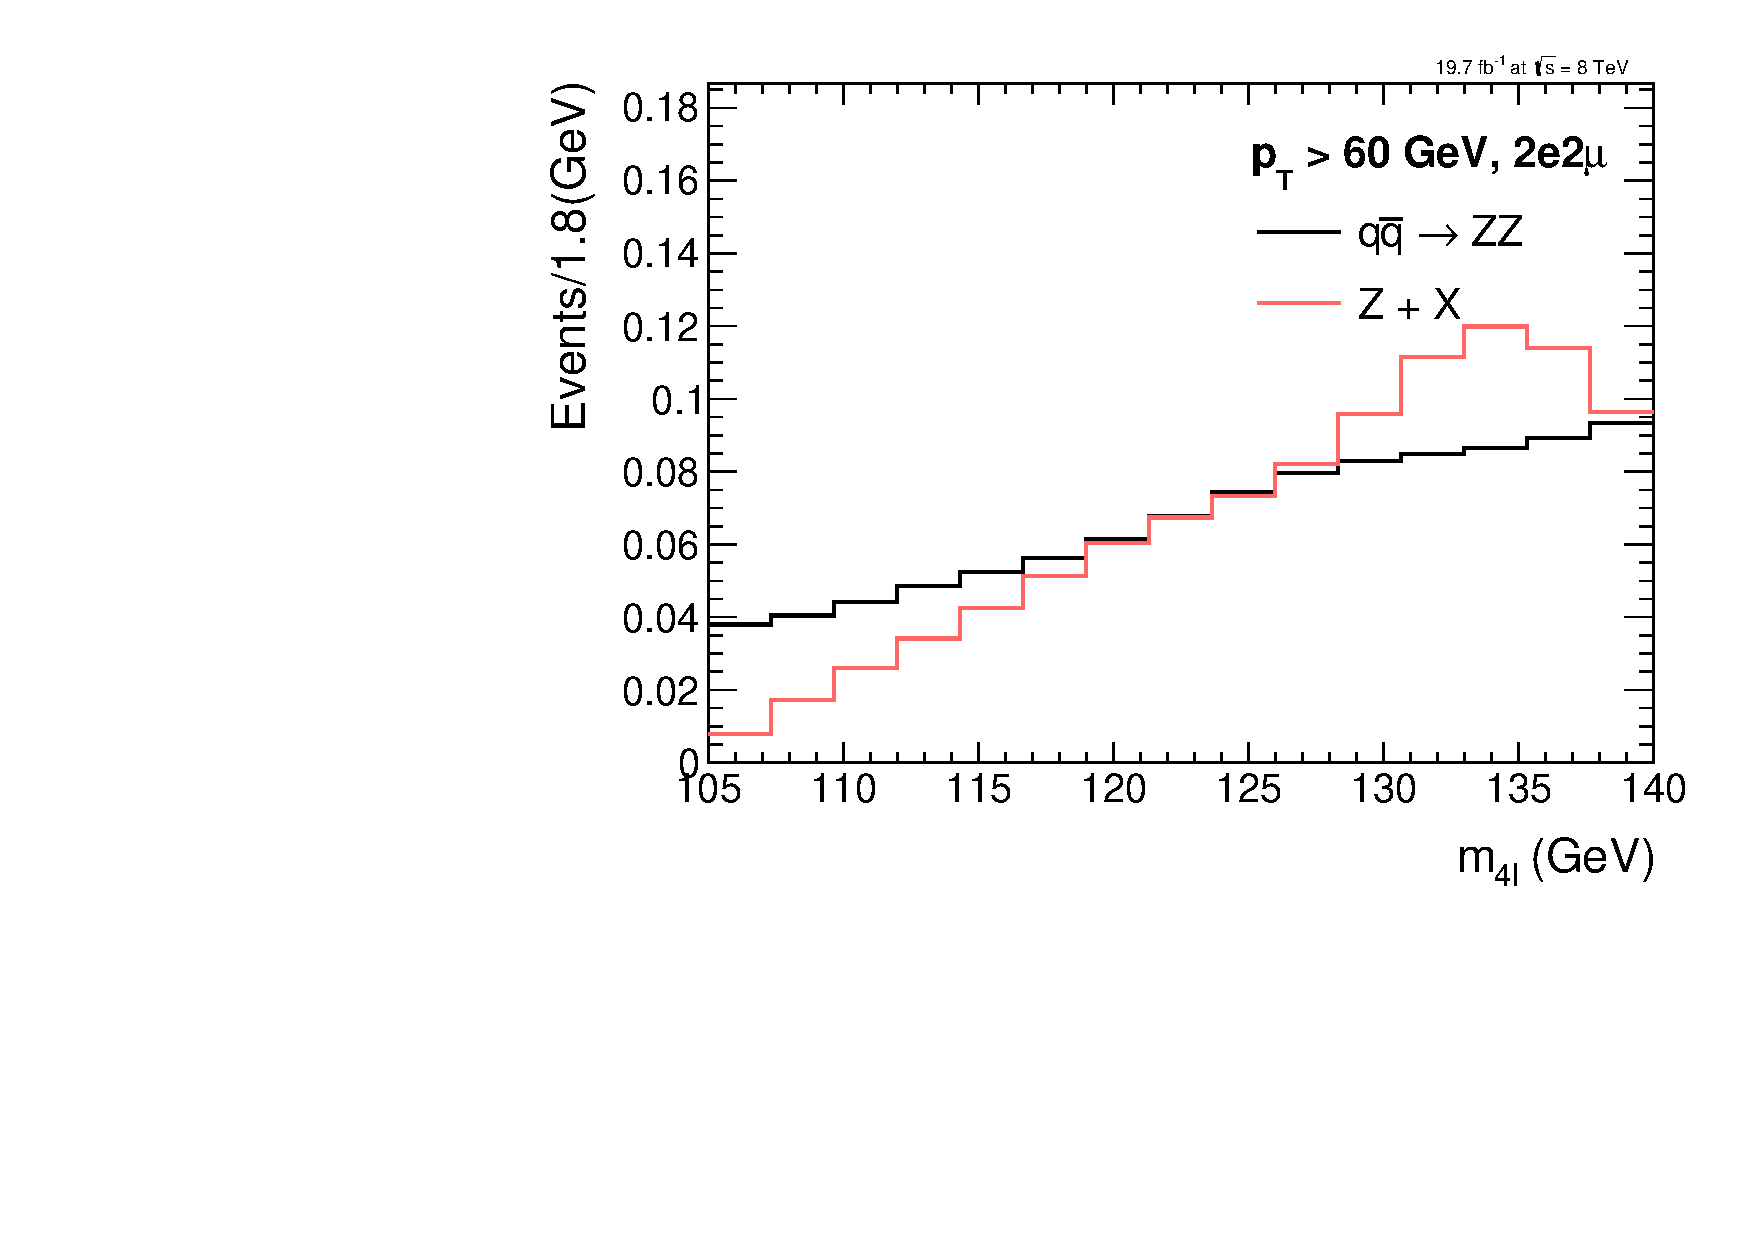
\includegraphics[width=0.3\textwidth,angle=0]{Appendix/figures/XSTemplates_2e2mu_pT4l_60_200_qqZZ_ZJetsCR.pdf}
%%    }
%%    \subfigure[$60.0 < \pt(4\ell) < 200.0$]{
%%      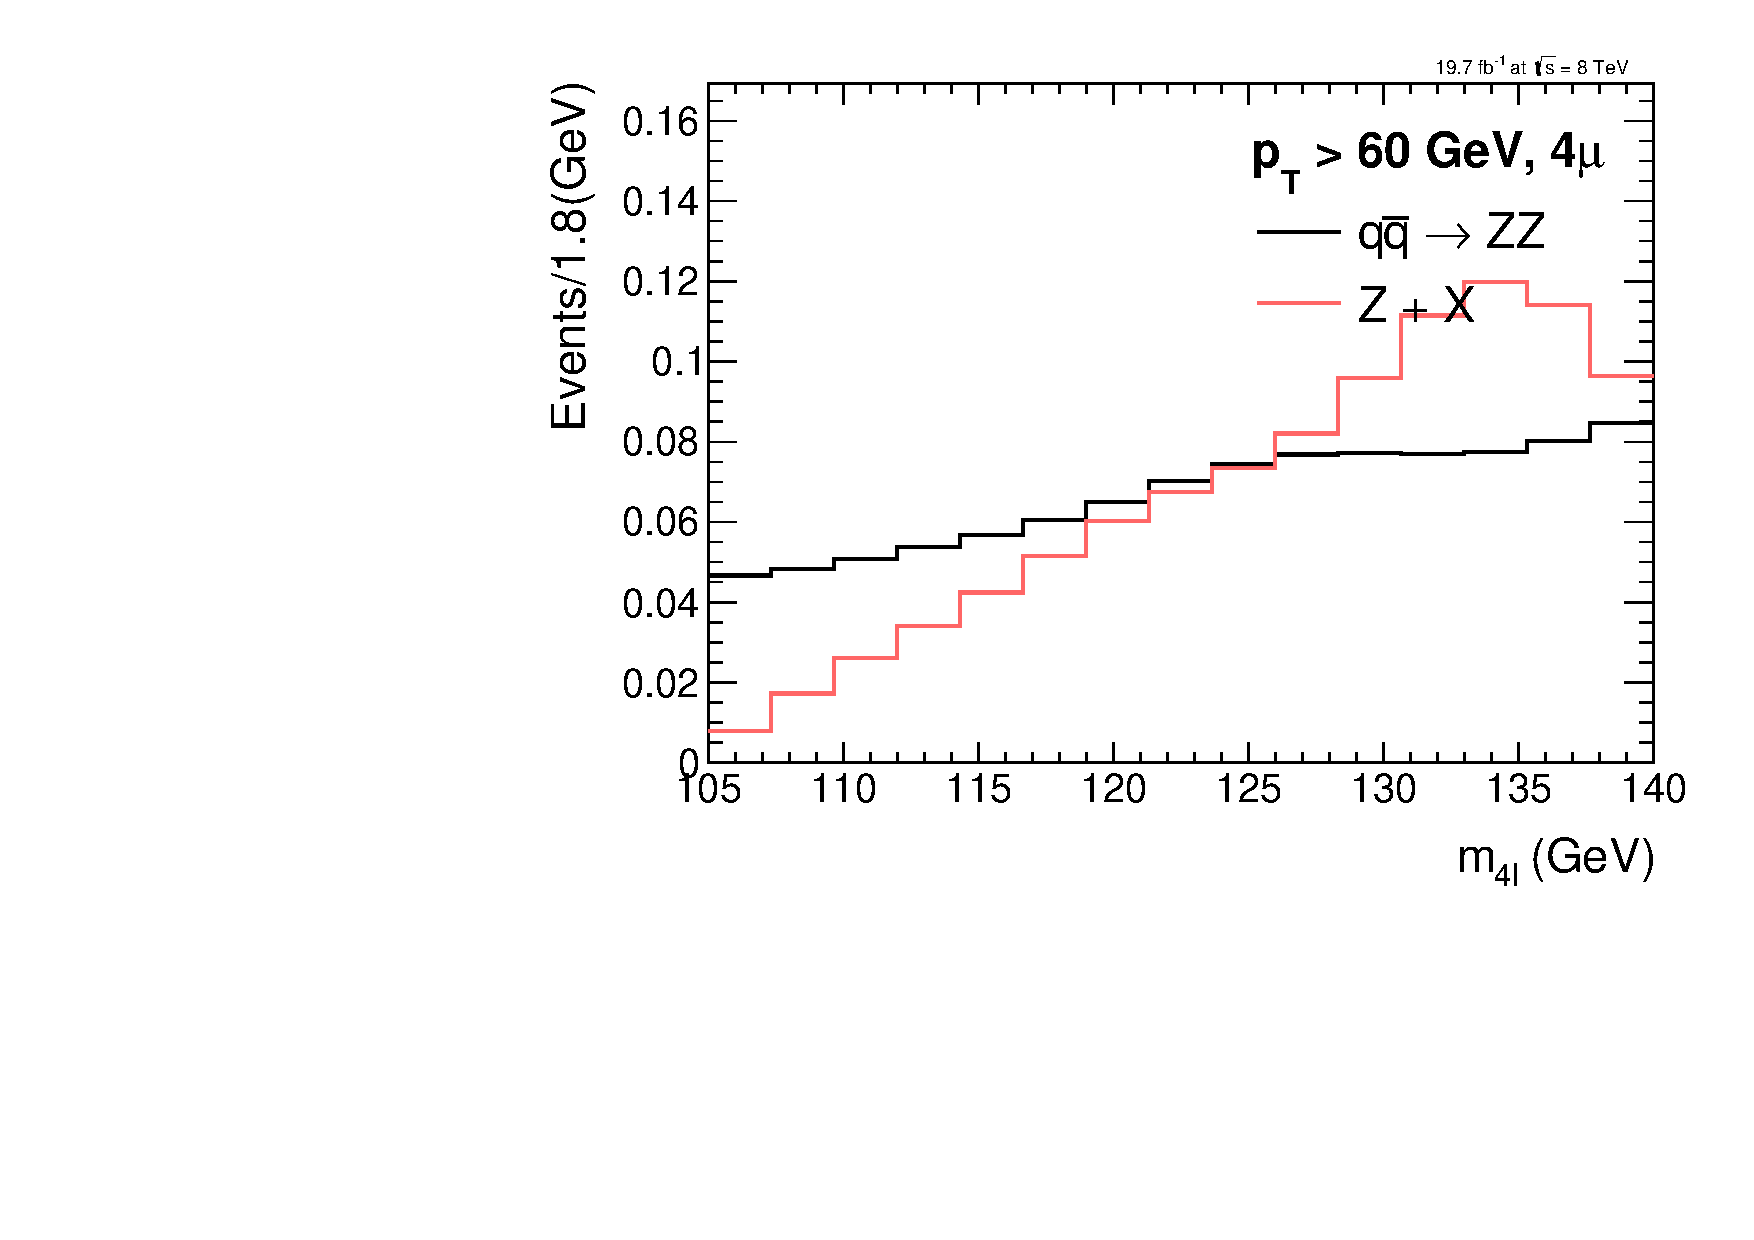
\includegraphics[width=0.3\textwidth,angle=0]{Appendix/figures/XSTemplates_4mu_pT4l_60_200_qqZZ_ZJetsCR.pdf}
%%    }
%%    \subfigure[$60.0 < \pt(4\ell) < 200.0$]{
%%      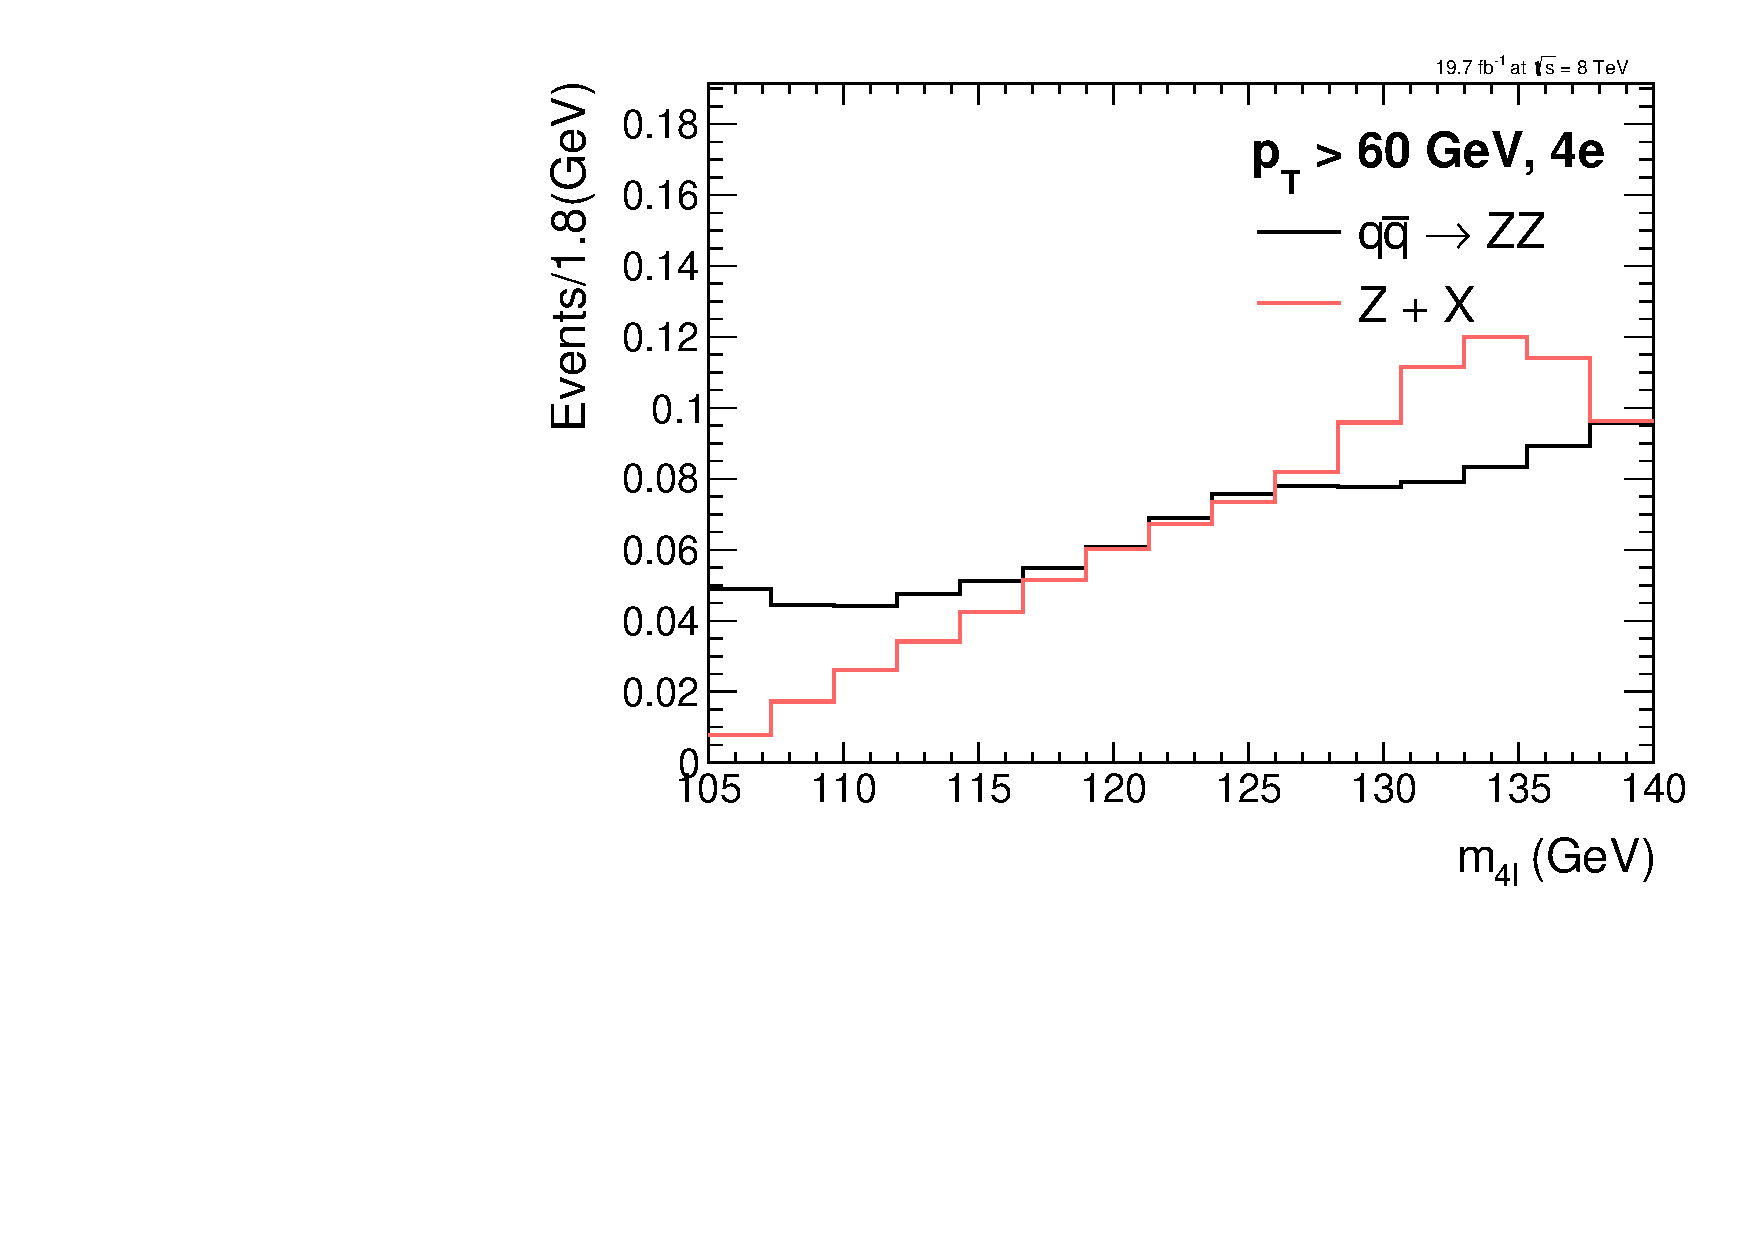
\includegraphics[width=0.3\textwidth,angle=0]{Appendix/figures/XSTemplates_4e_pT4l_60_200_qqZZ_ZJetsCR.pdf}
%%    } \\
%%
%%    \caption{ Distributions of m($4\ell$) for the $qq \rightarrow \mathrm{ZZ}$ and Z+X backgrounds in different bins of $\pt(4\ell)$
%%    for three final states: $2e2\mu$(left), $4\mu$(middle) and $4e$(right).}
%%  \label{fig:bkg-pT4l-qqZZ-ZX-main}
%%
%% \end{center}
%%\end{figure}
%
%%\clearpage

\subsubsection{Applying the Statistical Procedure} \label{sec:SignalDifferential}
The fiducial differential cross section is extracted in the bins of kinematic observables at the fiducial level following the procedure outlined in previous. 
For signal yields, mass spectrum of signal is built in each cell of the response matrix using a Double Crytal Ball (DCB) function, similar to what was done in Ref.~\cite{Chatrchyan:2013mxa}.
In practice, the same parameters of the CB function are used in each cell and the systematic uncertainties assigned on the energy scale and resolution generally cover discrepancy of signal mass spectrum among each cell.
\par
Examples of the fitted signal line shapes for differential bins of $\pt({\rm H})$ from gg$\rightarrow$H ({\sc powheg + JHUgen} 125 $\GeV$ 2018 sample) in the individual
final states are shown in Figure~\ref{fig:sigfits-pT4l-ggH-powheg15-JHUgen-125-maintext}, and examples of the efficiency matrices for $\pt({\rm H})$ for the
$2e2\mu$ final state are shown in Fig~\ref{fig:eff-pT4l-2e2mu-maintext}. Many more examples can be seen in Appendix~\ref{signalinputs}.

Figure~\ref{fig:sigfits-asimov-SM-pt4l-4l} shows the four lepton mass distributions for an Asimov dataset generated using SM cross section values and efficiencies
from the gg$\rightarrow$H production mode from {\sc powheg+JHUgen}, and resulting fitted values of PDFs of signal and background for different bins of $\pt(\mathrm{H})$ (all final states combined).

%%%%%%%%%5
\begin{figure}[htb]
  \begin{center}
    \subfigure[$0.0 < \pt(\mathrm{H}) < 15.0 $]{
      %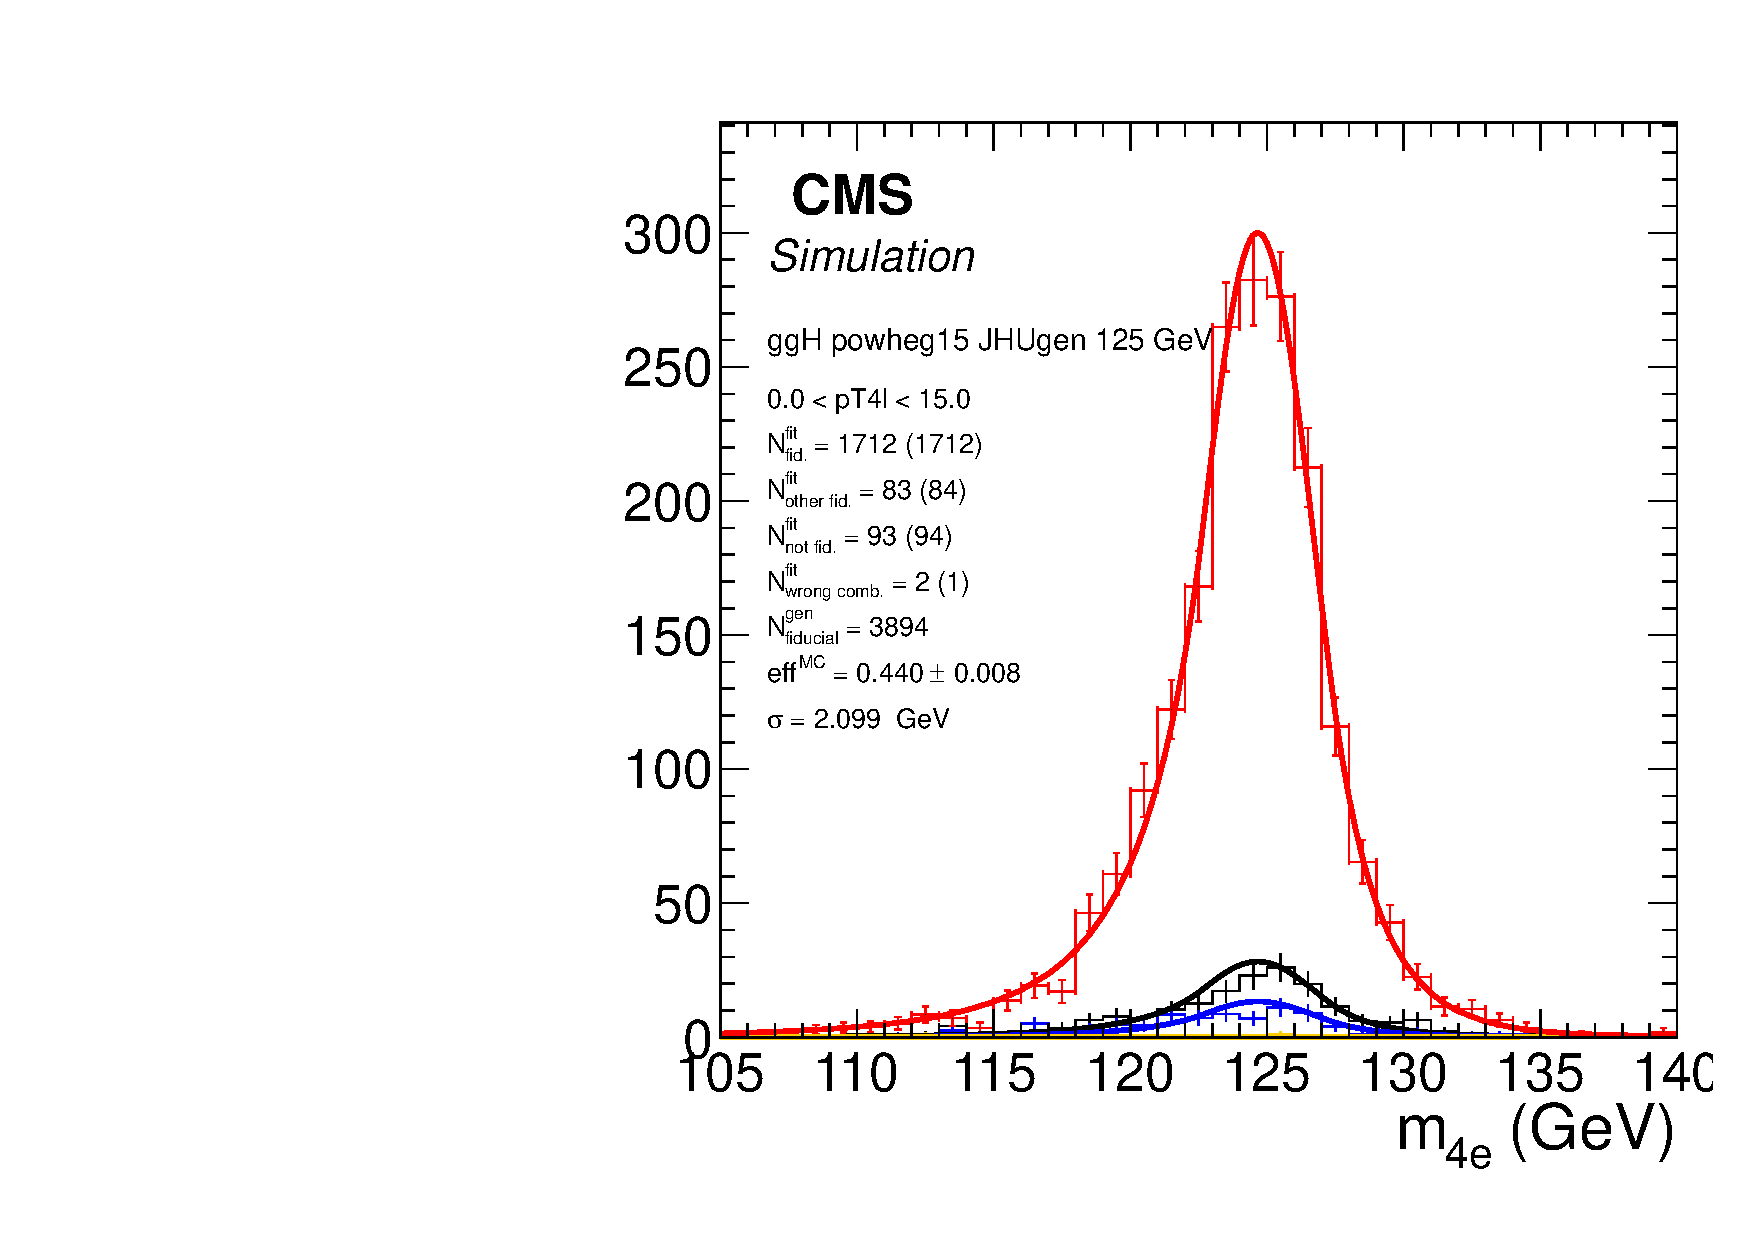
\includegraphics[width=0.3\textwidth,angle=0]{Figures/results/fiducial/2018//ggH_powheg15_JHUgen_125_4e_pT4l_genbin0_recobin0_effs_eventMCWeight.pdf}
      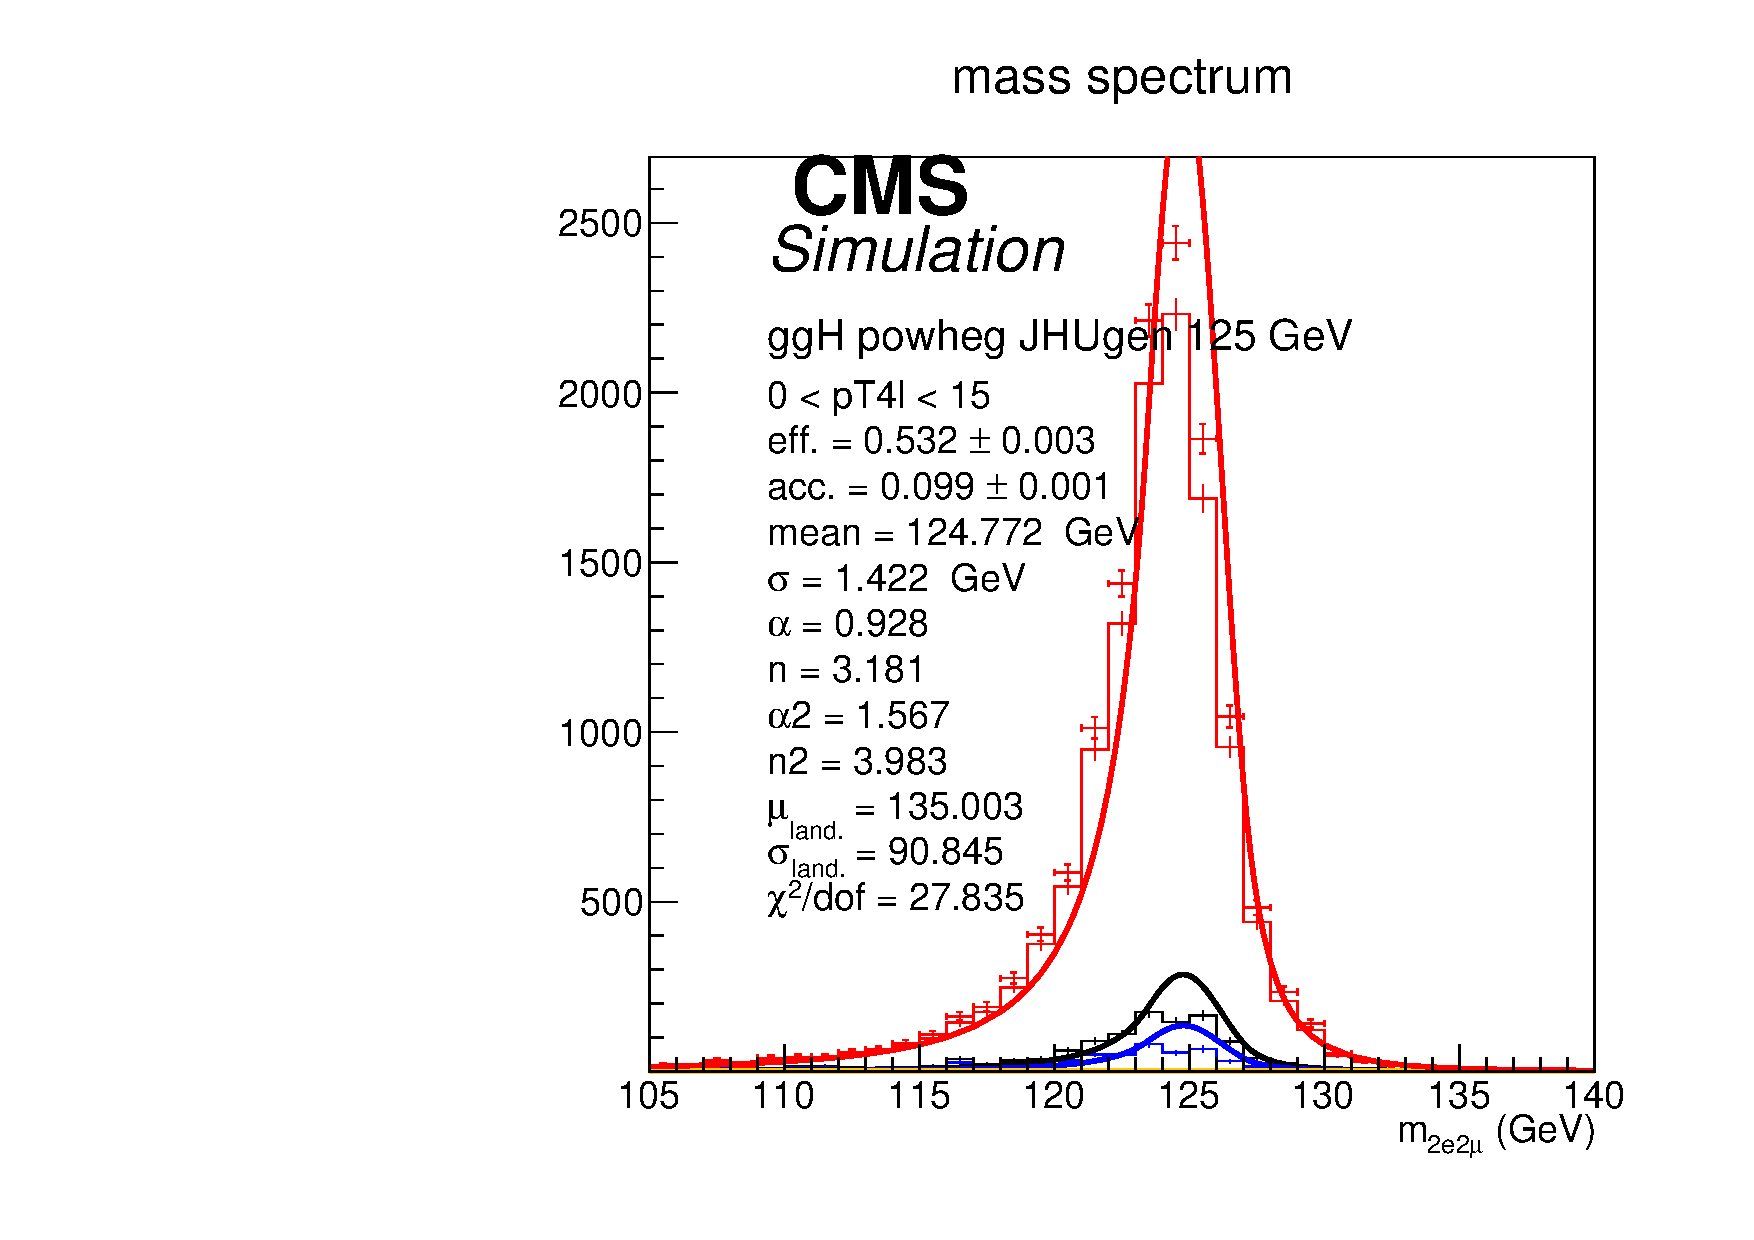
\includegraphics[width=0.3\textwidth,angle=0]{Figures/results/fiducial/2018//ggH_powheg_JHUgen_125_2e2mu_pT4l_genbin0_recobin0_effs_genWeight*pileupWeight*dataMCWeight.pdf}
      \label{fig:sigfits-pT4l-ggH-powheg15-JHUgen-125-maintext:a}
    }
    \subfigure[$15.0 < \pt(\mathrm{H}) < 30.0$]{
      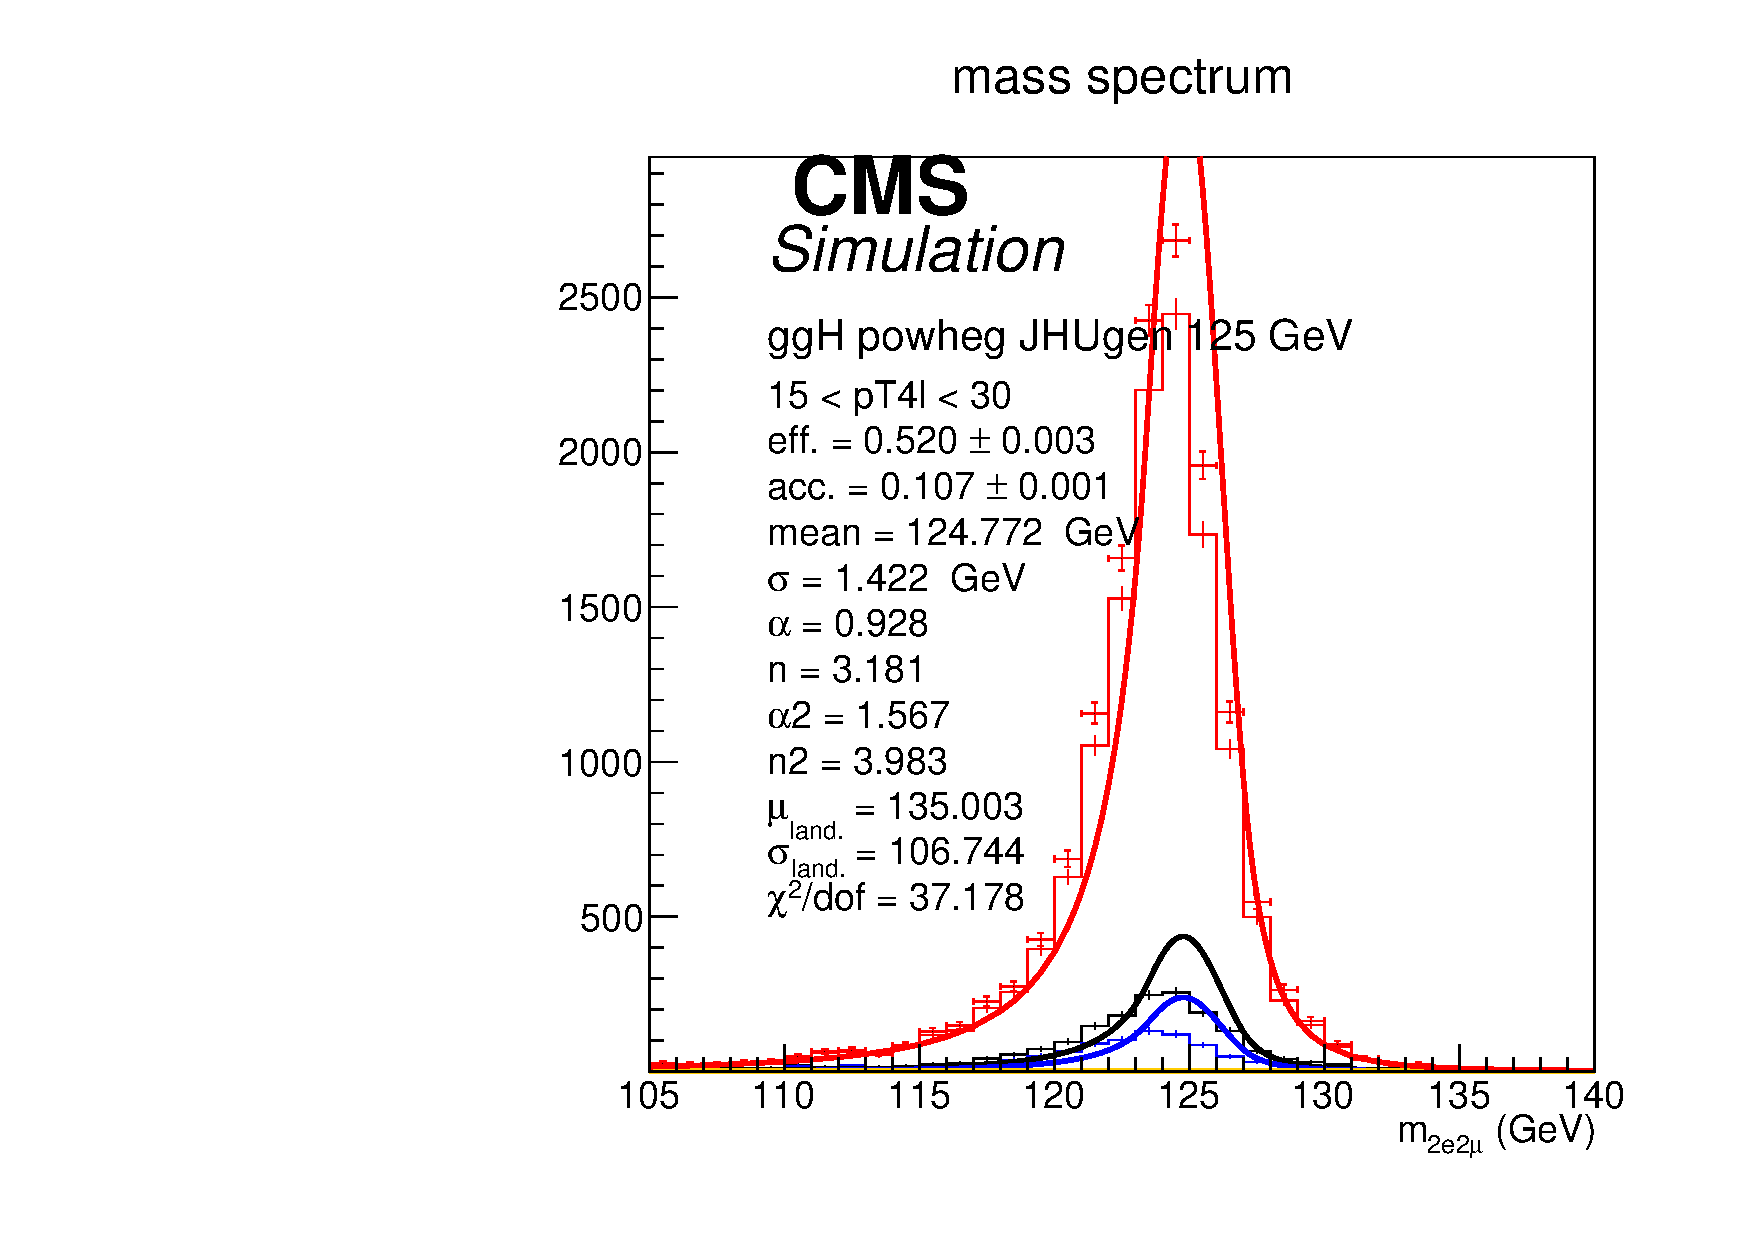
\includegraphics[width=0.3\textwidth,angle=0]{Figures/results/fiducial/2018//ggH_powheg_JHUgen_125_2e2mu_pT4l_genbin1_recobin1_effs_genWeight*pileupWeight*dataMCWeight.pdf}
      \label{fig:sigfits-pT4l-ggH-powheg15-JHUgen-125-maintext:b}
    }
   \subfigure[$30.0 < \pt(\mathrm{H}) < 45.0$]{
      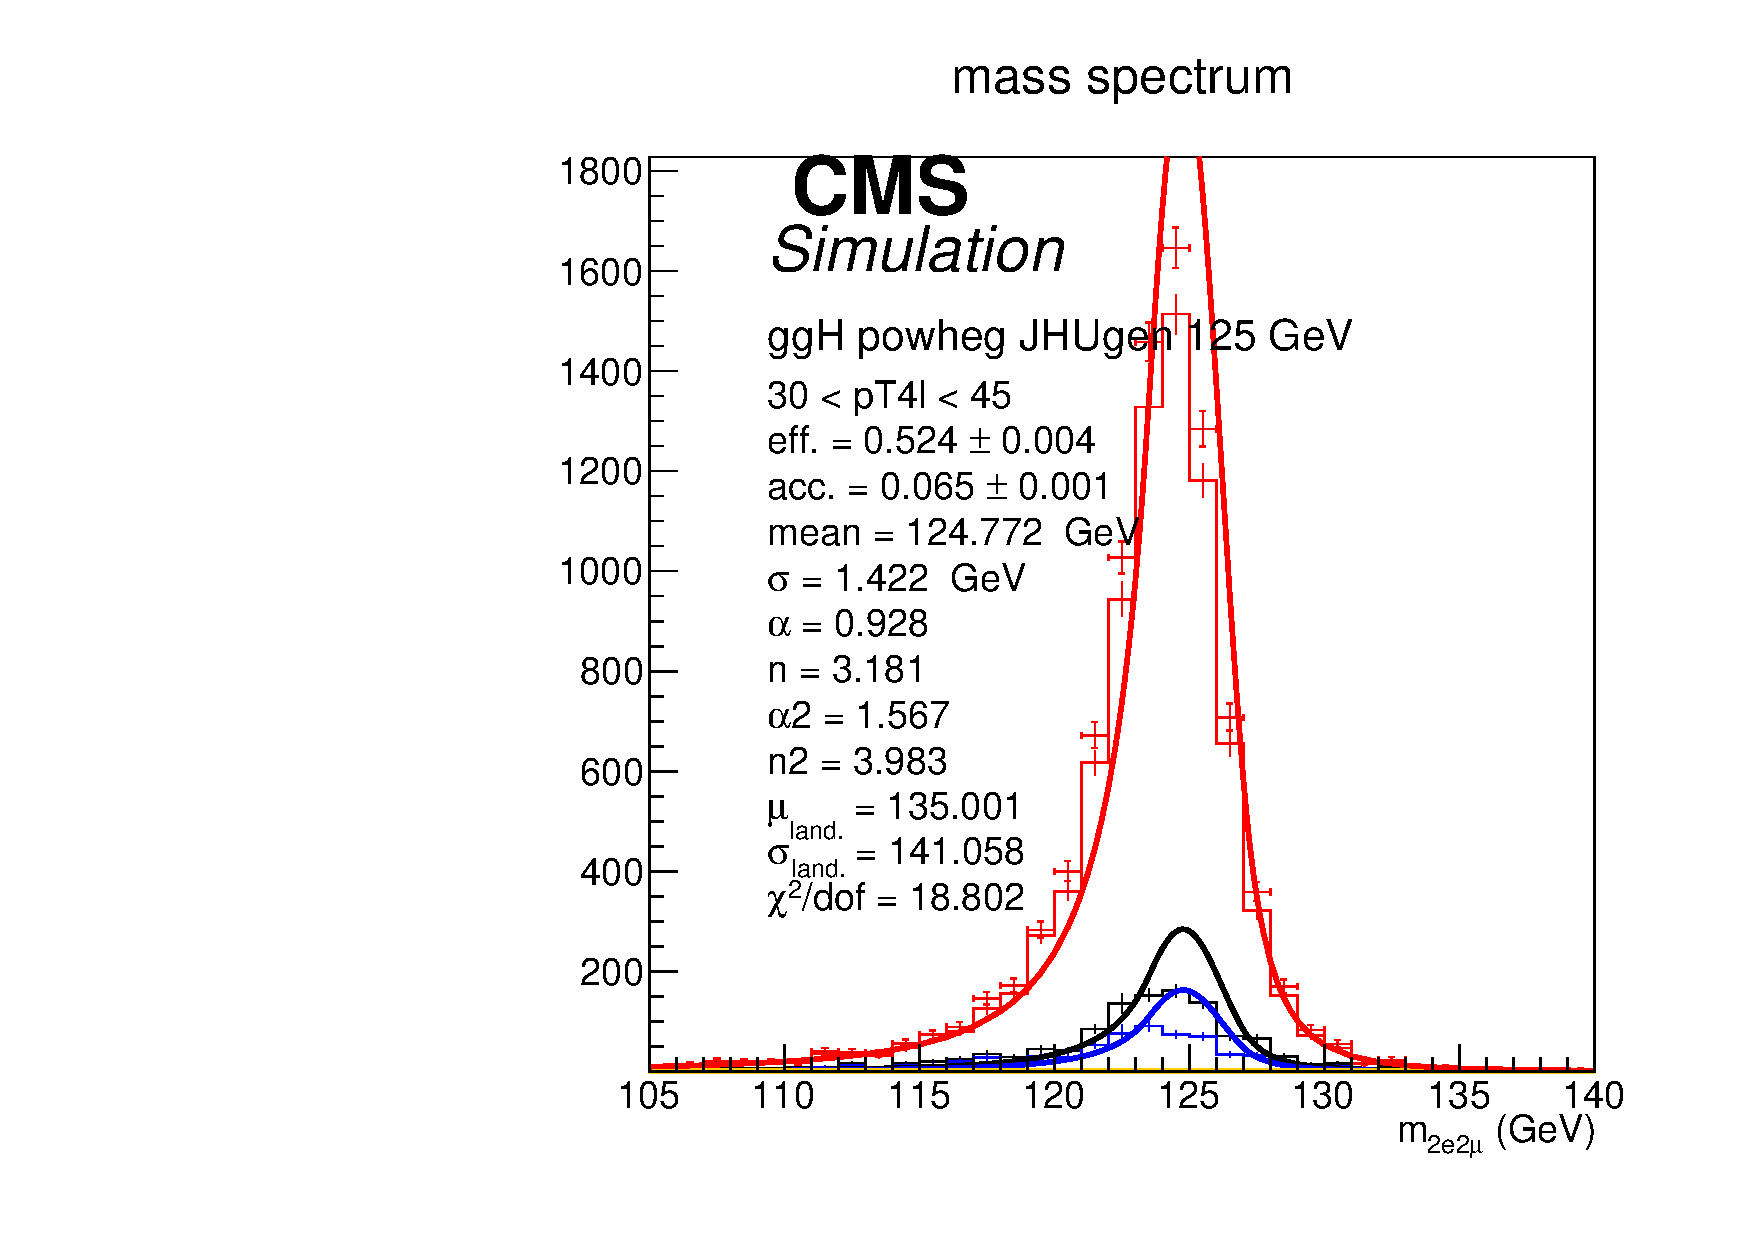
\includegraphics[width=0.3\textwidth,angle=0]{Figures/results/fiducial/2018//ggH_powheg_JHUgen_125_2e2mu_pT4l_genbin2_recobin2_effs_genWeight*pileupWeight*dataMCWeight.pdf}
      \label{fig:sigfits-pT4l-ggH-powheg15-JHUgen-125-maintext:c}
    }  \\
    \subfigure[$45.0 < \pt(\mathrm{H}) < 80.0$]{
      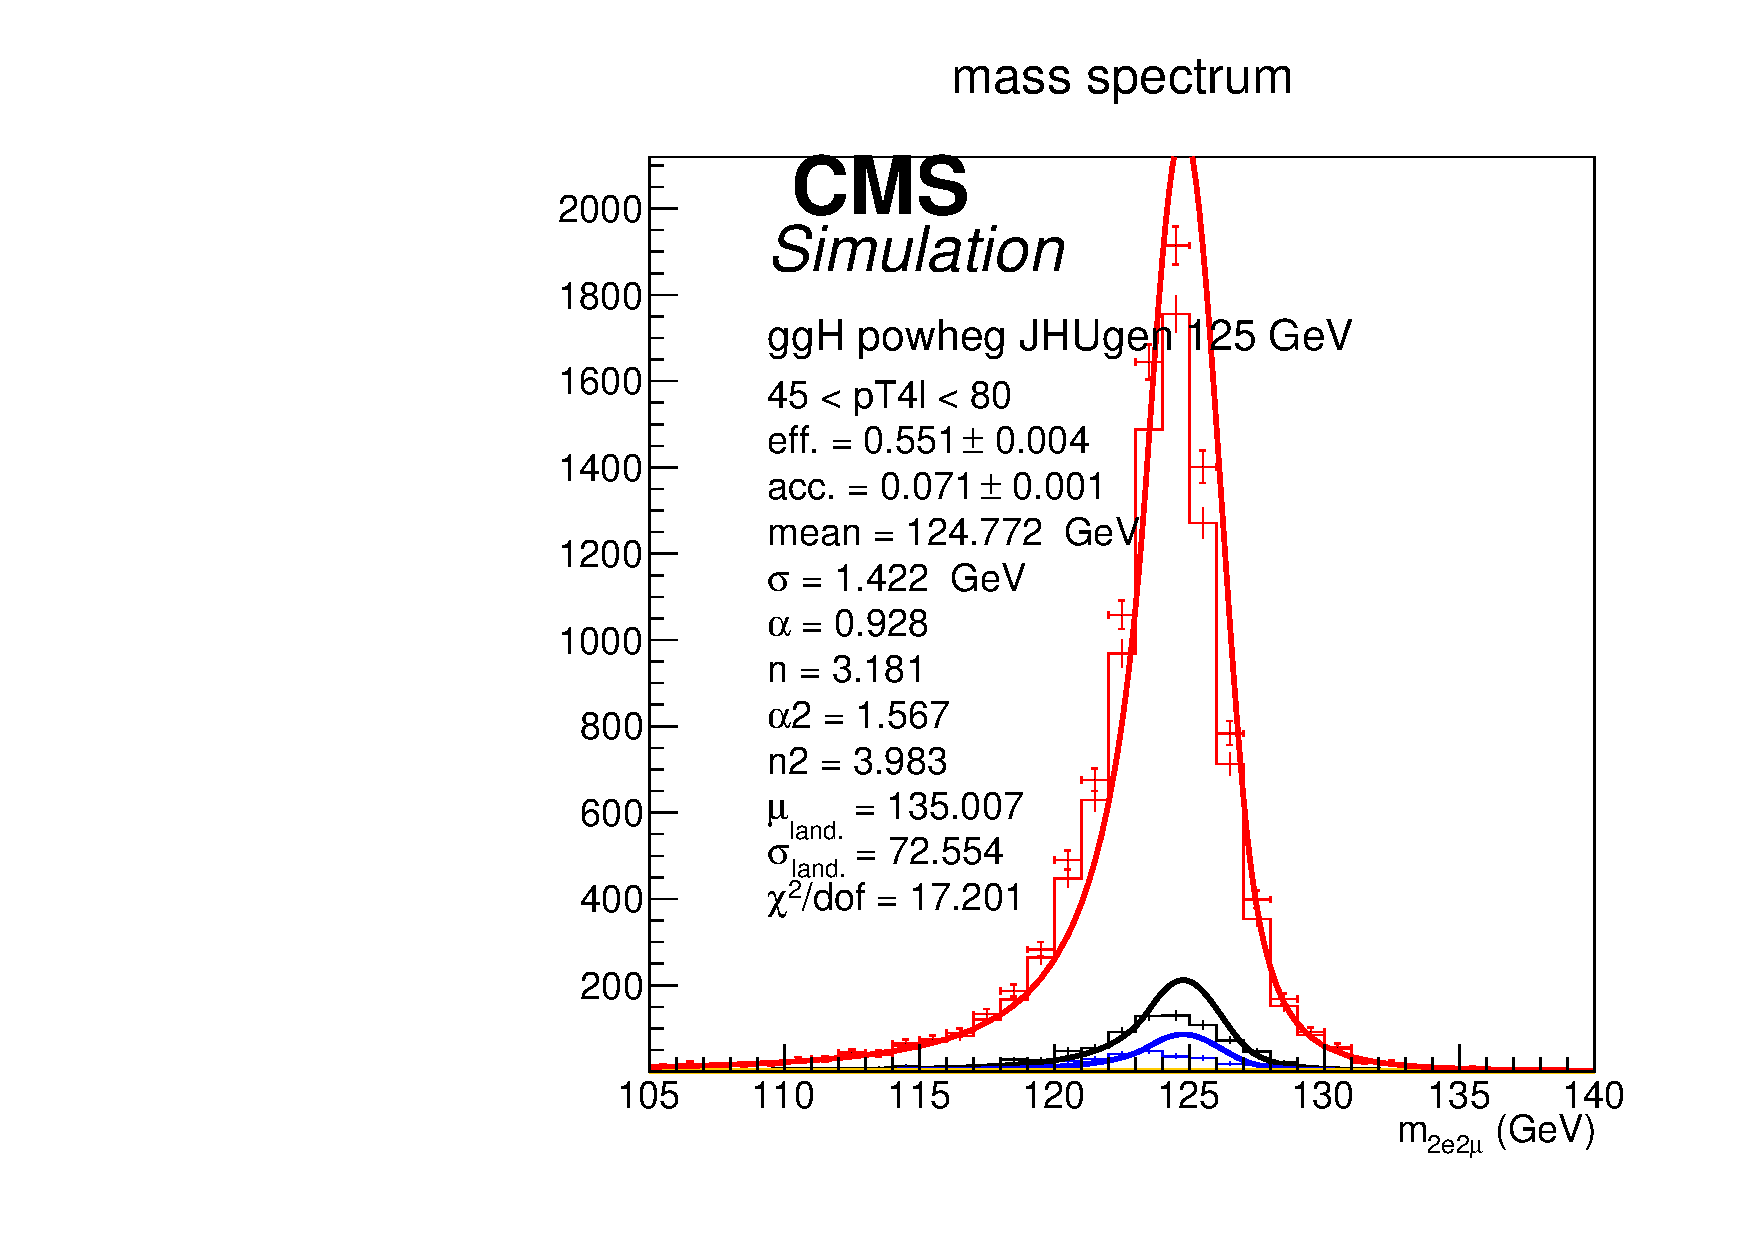
\includegraphics[width=0.3\textwidth,angle=0]{Figures/results/fiducial/2018//ggH_powheg_JHUgen_125_2e2mu_pT4l_genbin3_recobin3_effs_genWeight*pileupWeight*dataMCWeight.pdf}
      \label{fig:sigfits-pT4l-ggH-powheg15-JHUgen-125-maintext:d}
    }
    \subfigure[$80.0 < \pt(\mathrm{H}) < 120.0$]{
      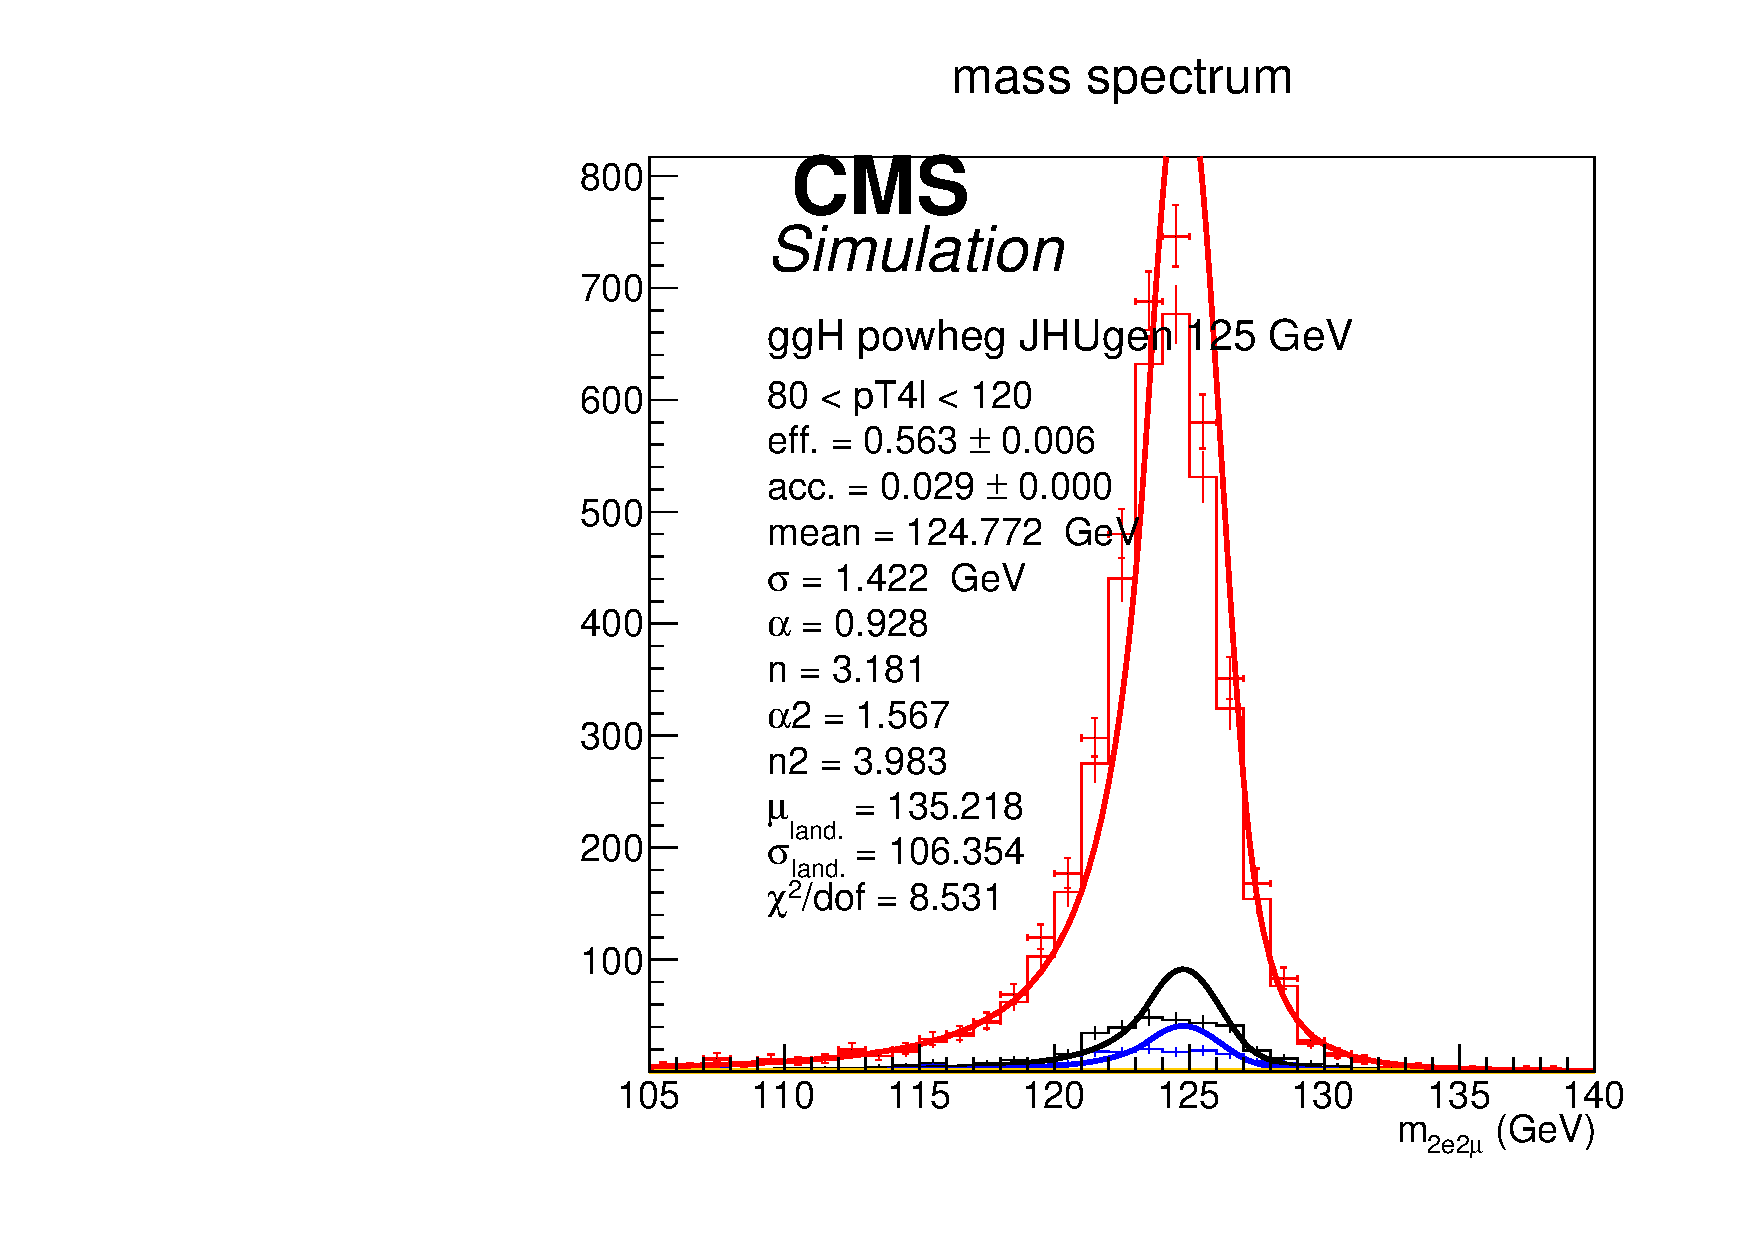
\includegraphics[width=0.3\textwidth,angle=0]{Figures/results/fiducial/2018//ggH_powheg_JHUgen_125_2e2mu_pT4l_genbin4_recobin4_effs_genWeight*pileupWeight*dataMCWeight.pdf}
      \label{fig:sigfits-pT4l-ggH-powheg15-JHUgen-125-maintext:e}
    }
    \subfigure[$120.0 < \pt(\mathrm{H}) < 200.0$]{
      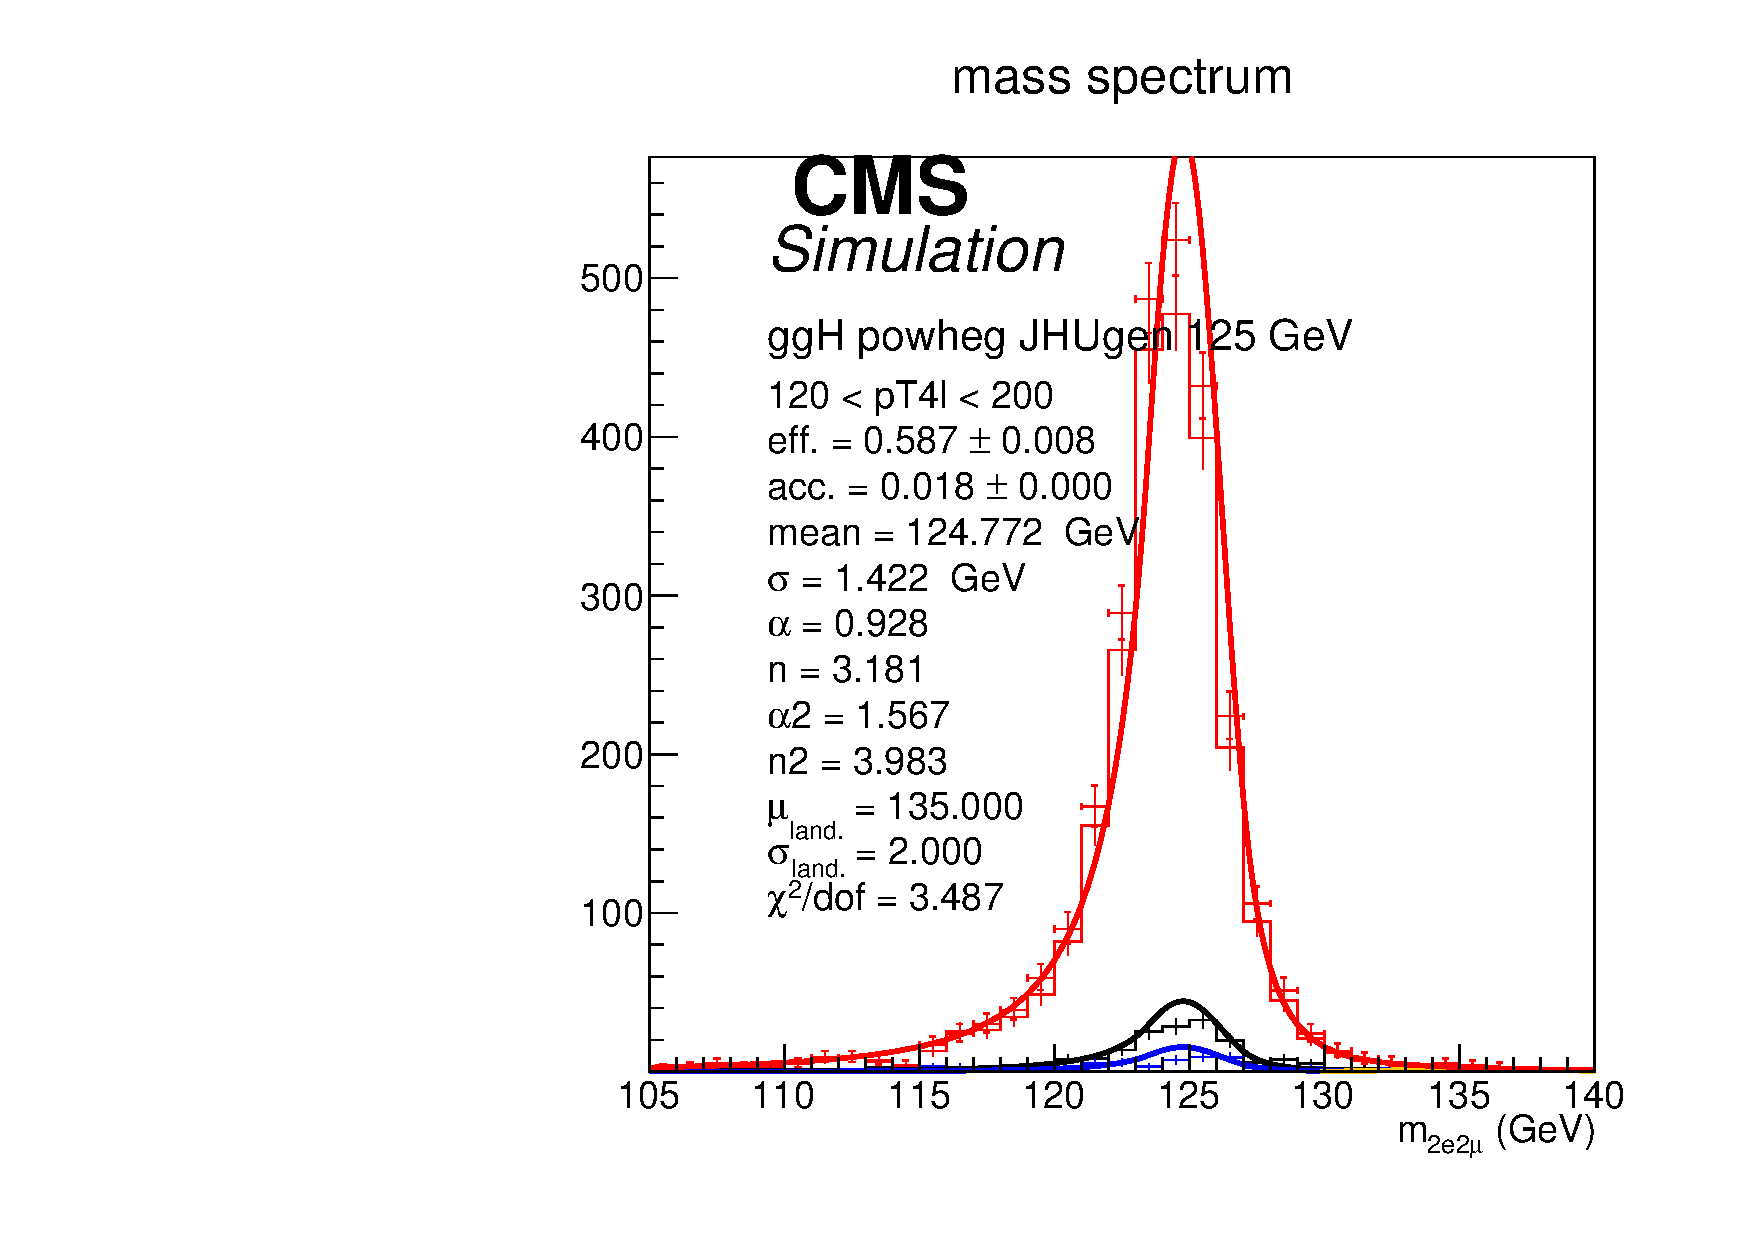
\includegraphics[width=0.3\textwidth,angle=0]{Figures/results/fiducial/2018//ggH_powheg_JHUgen_125_2e2mu_pT4l_genbin5_recobin5_effs_genWeight*pileupWeight*dataMCWeight.pdf}
      \label{fig:sigfits-pT4l-ggH-powheg15-JHUgen-125-maintext:f}
    } \\
    \subfigure[$200.0 < \pt(\mathrm{H}) < 13000.0$]{
      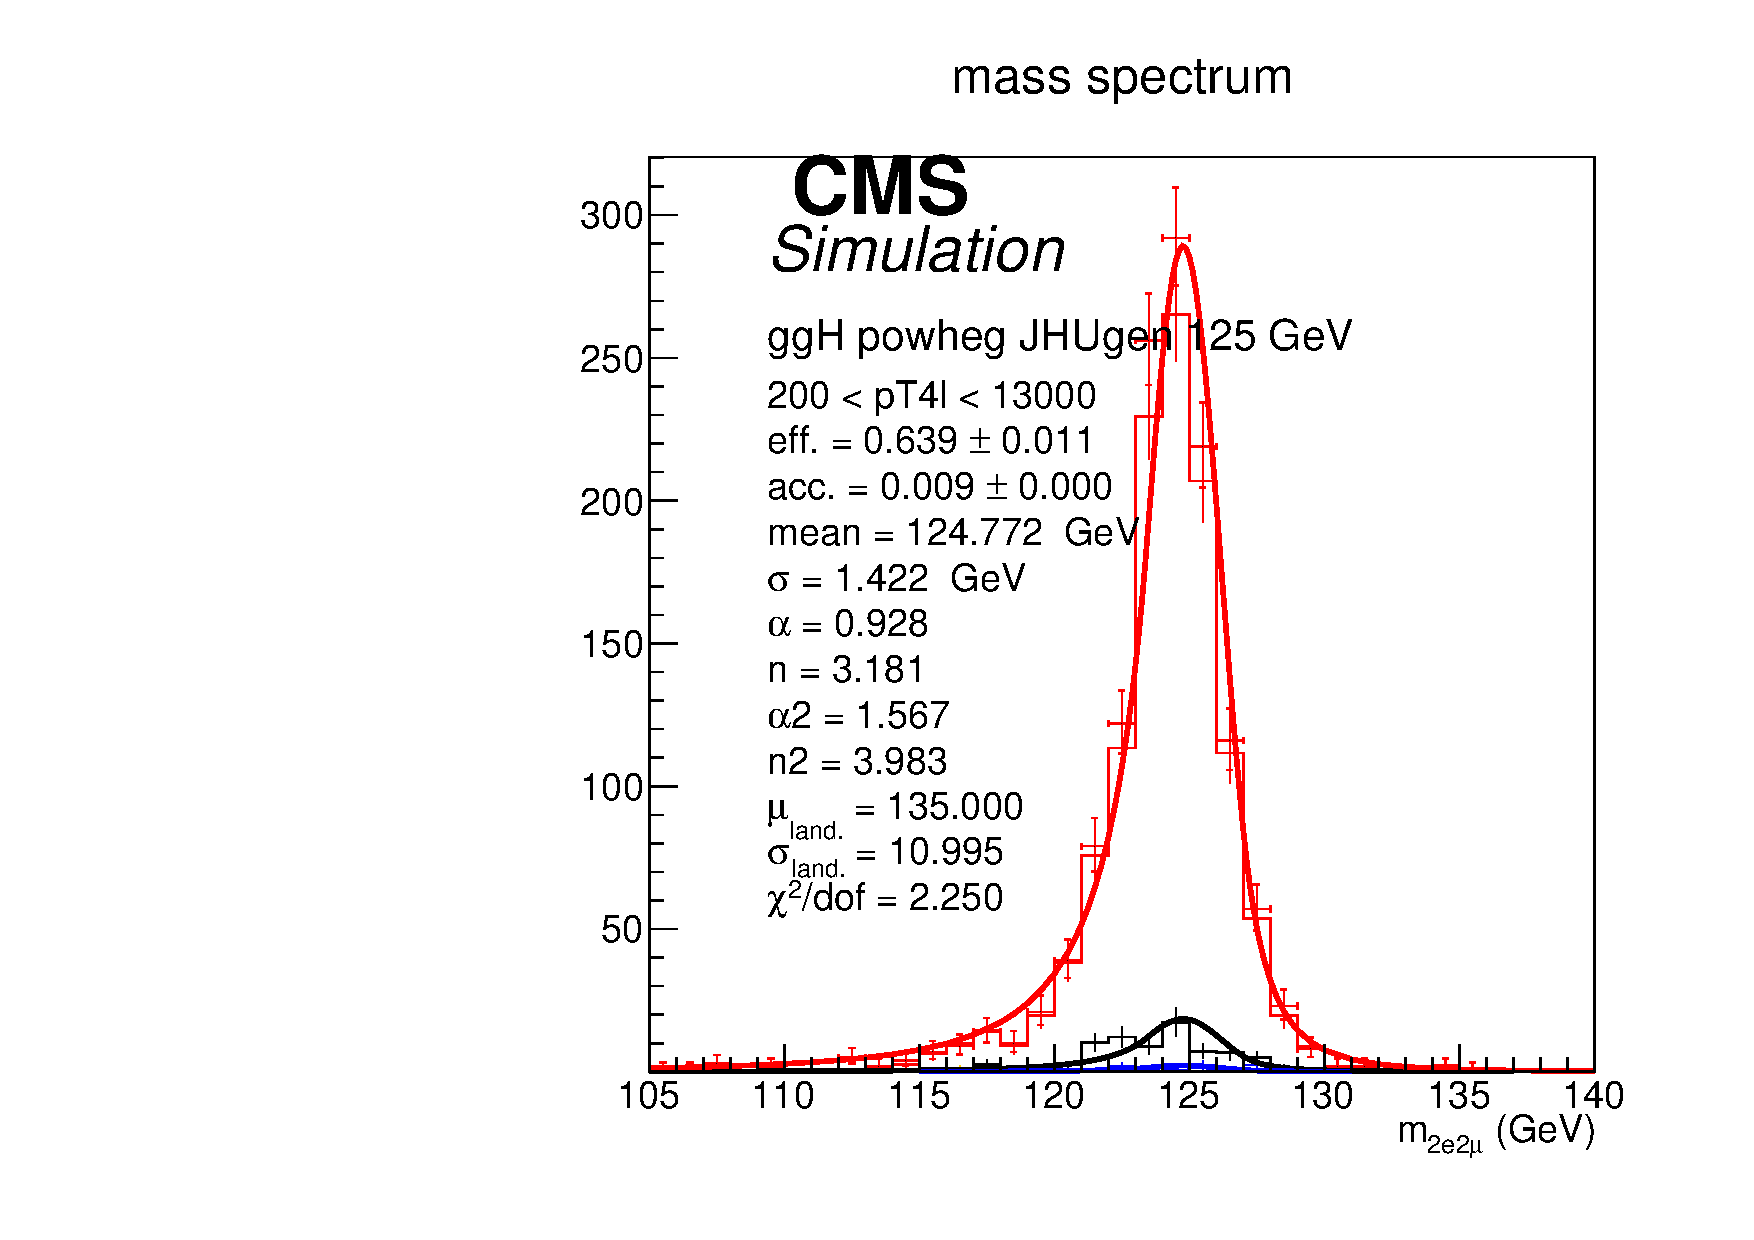
\includegraphics[width=0.3\textwidth,angle=0]{Figures/results/fiducial/2018//ggH_powheg_JHUgen_125_2e2mu_pT4l_genbin6_recobin6_effs_genWeight*pileupWeight*dataMCWeight.pdf}
      \label{fig:sigfits-pT4l-ggH-powheg15-JHUgen-125-maintext:g}
    }
%    \subfigure[$30.0 < \pt(\mathrm{H}) < 60.0$]{
%      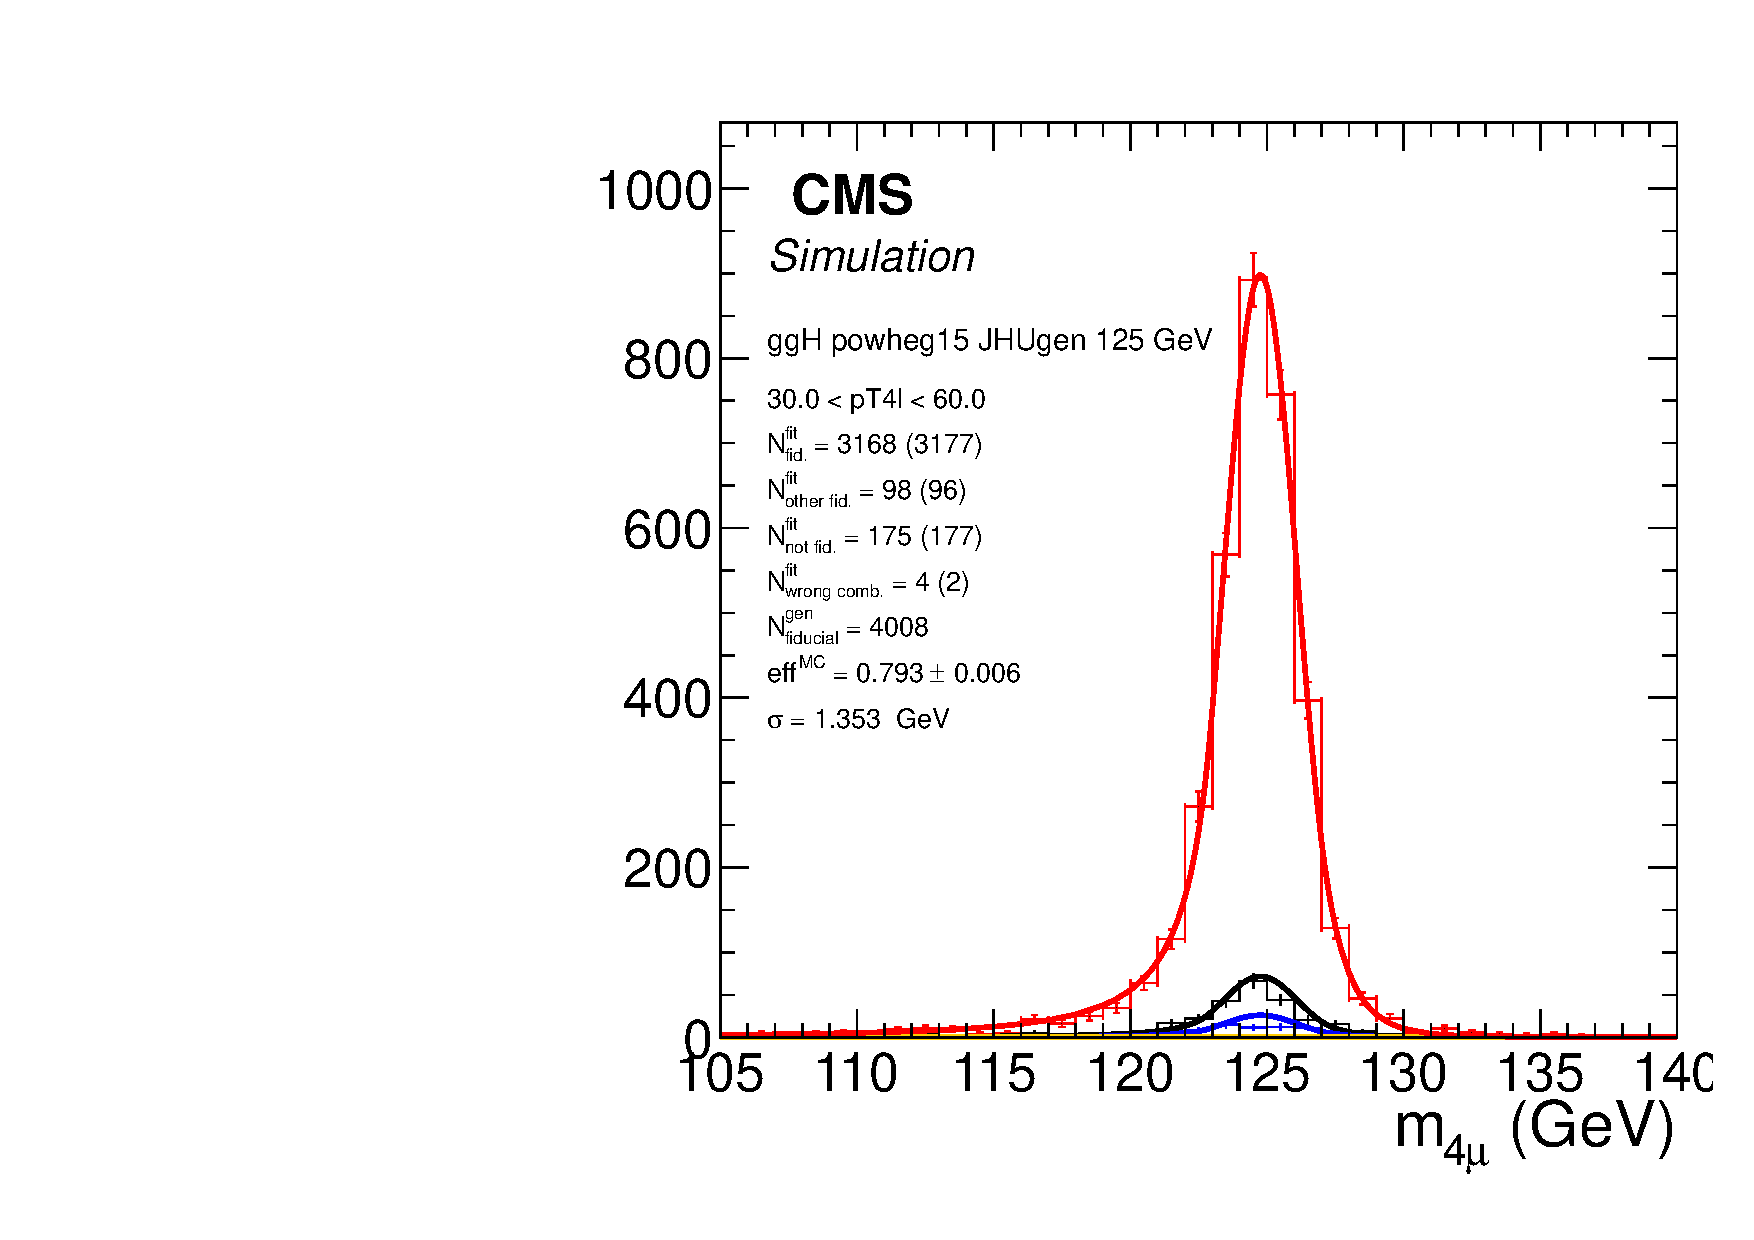
\includegraphics[width=0.3\textwidth,angle=0]{Figures/results/fiducial/2018//ggH_powheg15_JHUgen_125_4mu_pT4l_genbin2_recobin2_effs_eventMCWeight.pdf}
%      \label{fig:sigfits-pT4l-ggH-powheg15-JHUgen-125-maintext:h}
%    }
%    \subfigure[$30.0  < \pt(\mathrm{H}) < 60.0$]{
%      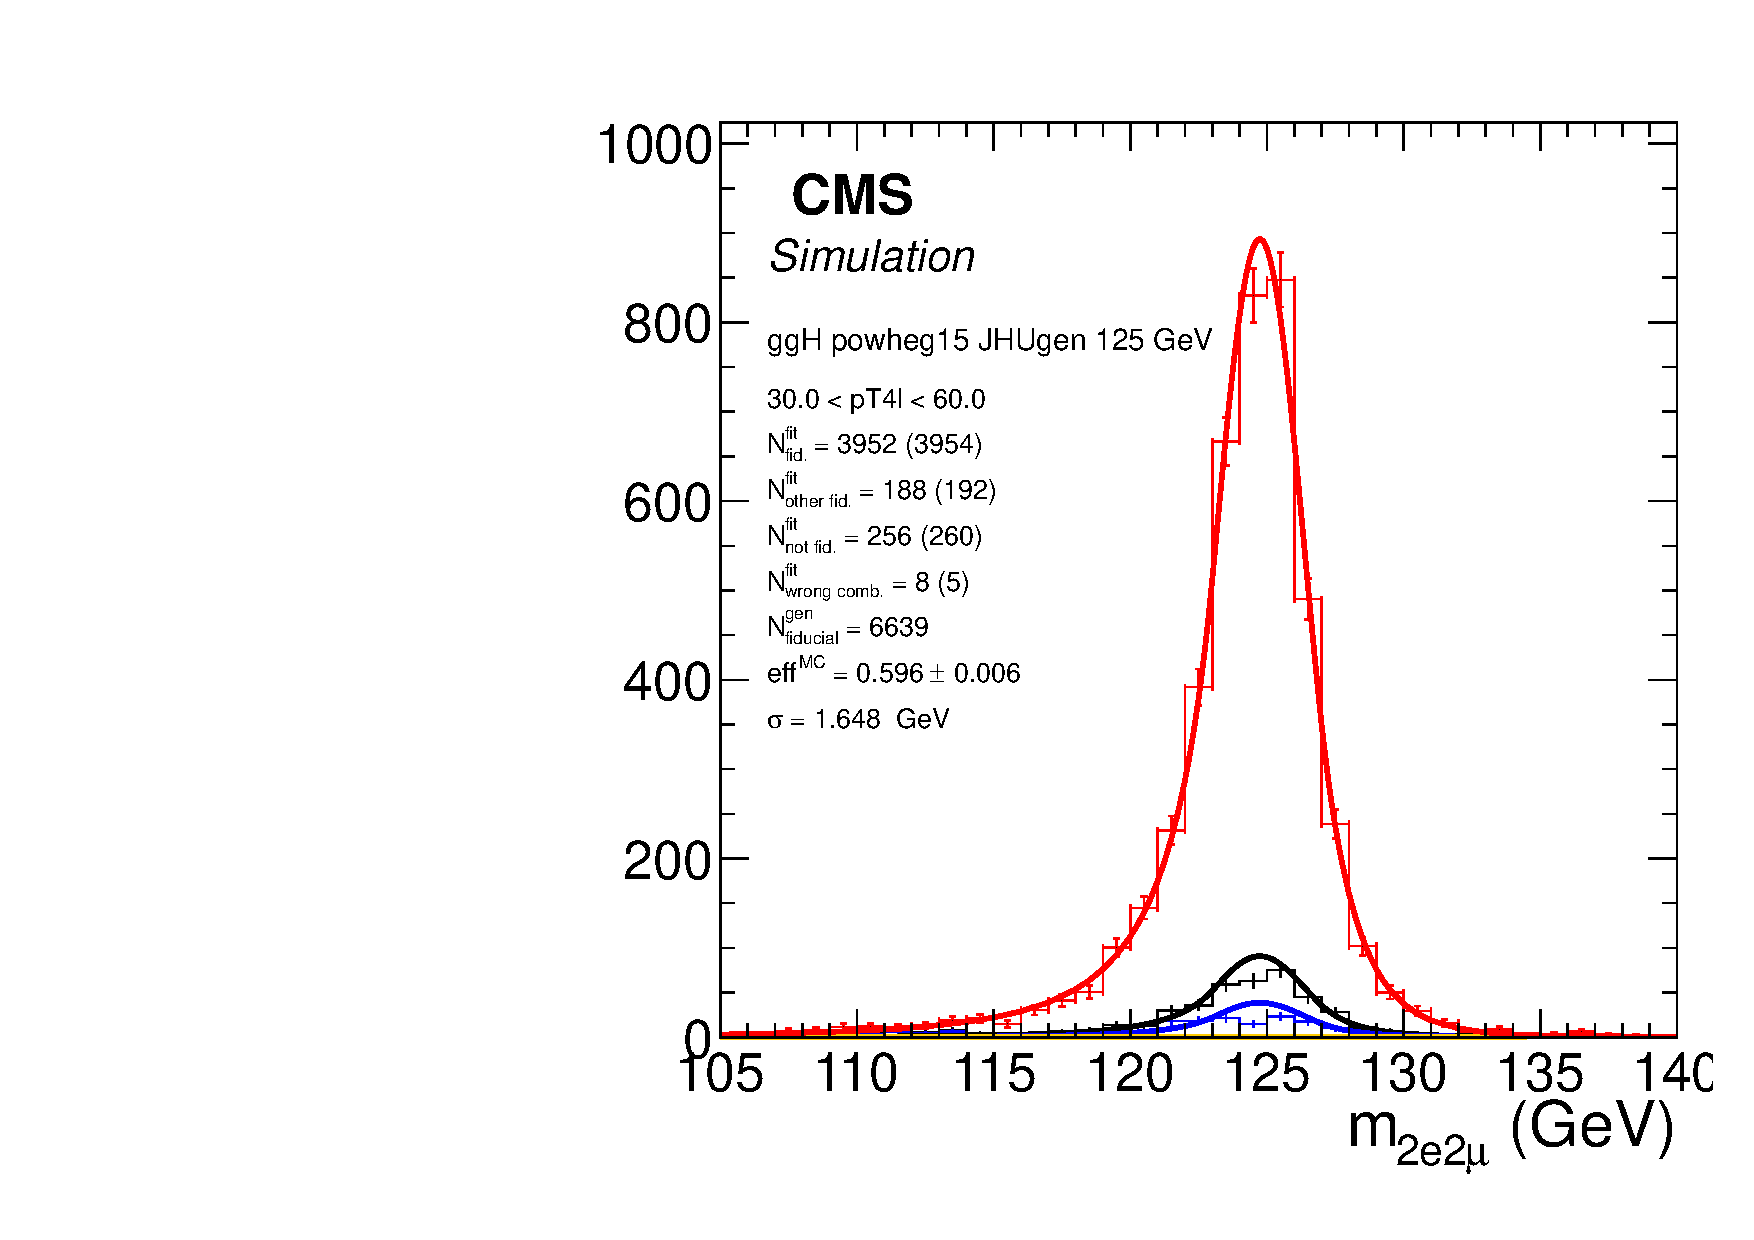
\includegraphics[width=0.3\textwidth,angle=0]{Figures/results/fiducial/2018//ggH_powheg15_JHUgen_125_2e2mu_pT4l_genbin2_recobin2_effs_eventMCWeight.pdf}
%      \label{fig:sigfits-pT4l-ggH-powheg15-JHUgen-125-maintext:i}
%    } \\
%    \subfigure[$60.0  < \pt(\mathrm{H}) < 200.0 $]{
%      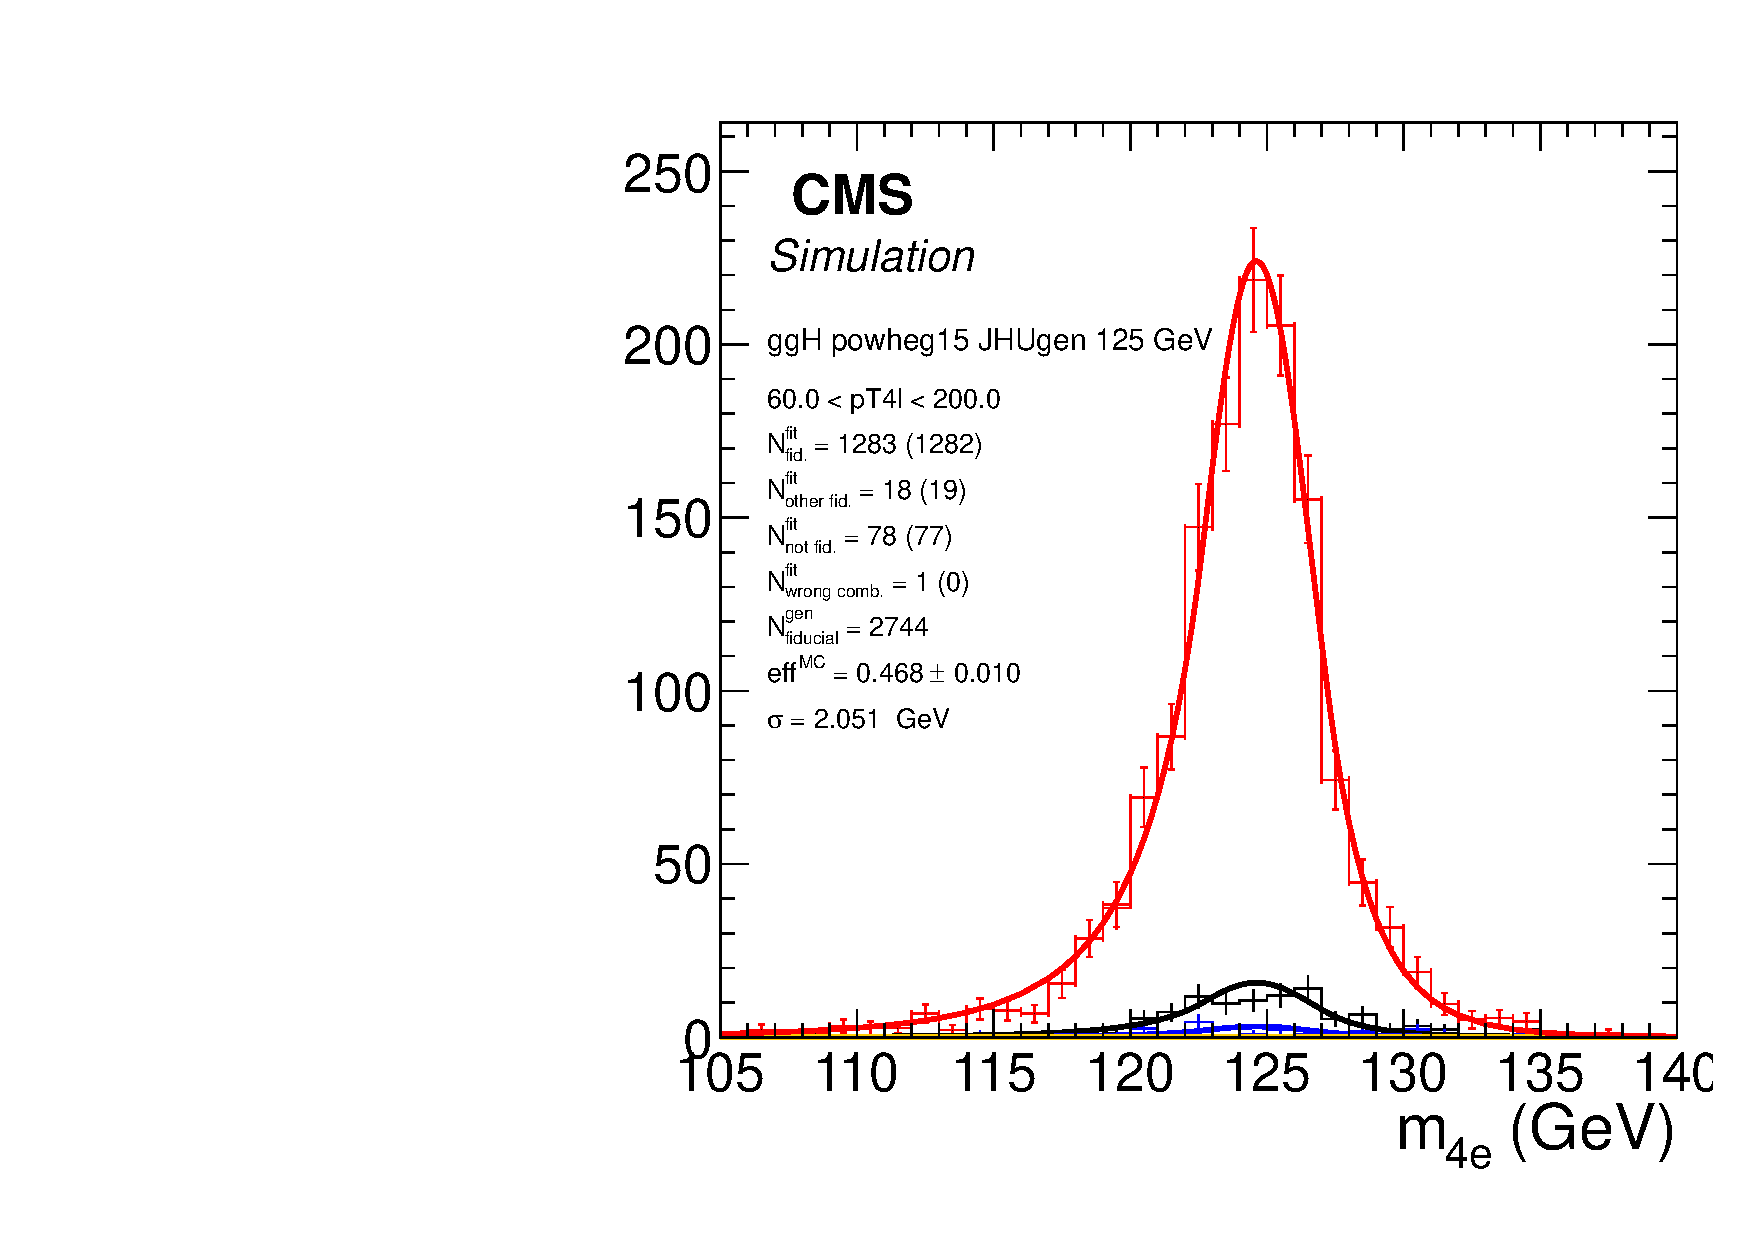
\includegraphics[width=0.3\textwidth,angle=0]{Figures/results/fiducial/2018//ggH_powheg15_JHUgen_125_4e_pT4l_genbin3_recobin3_effs_eventMCWeight.pdf}
%      \label{fig:sigfits-pT4l-ggH-powheg15-JHUgen-125-maintext:j}
%    }
%    \subfigure[$60.0  < \pt(\mathrm{H}) < 200.0 $]{
%      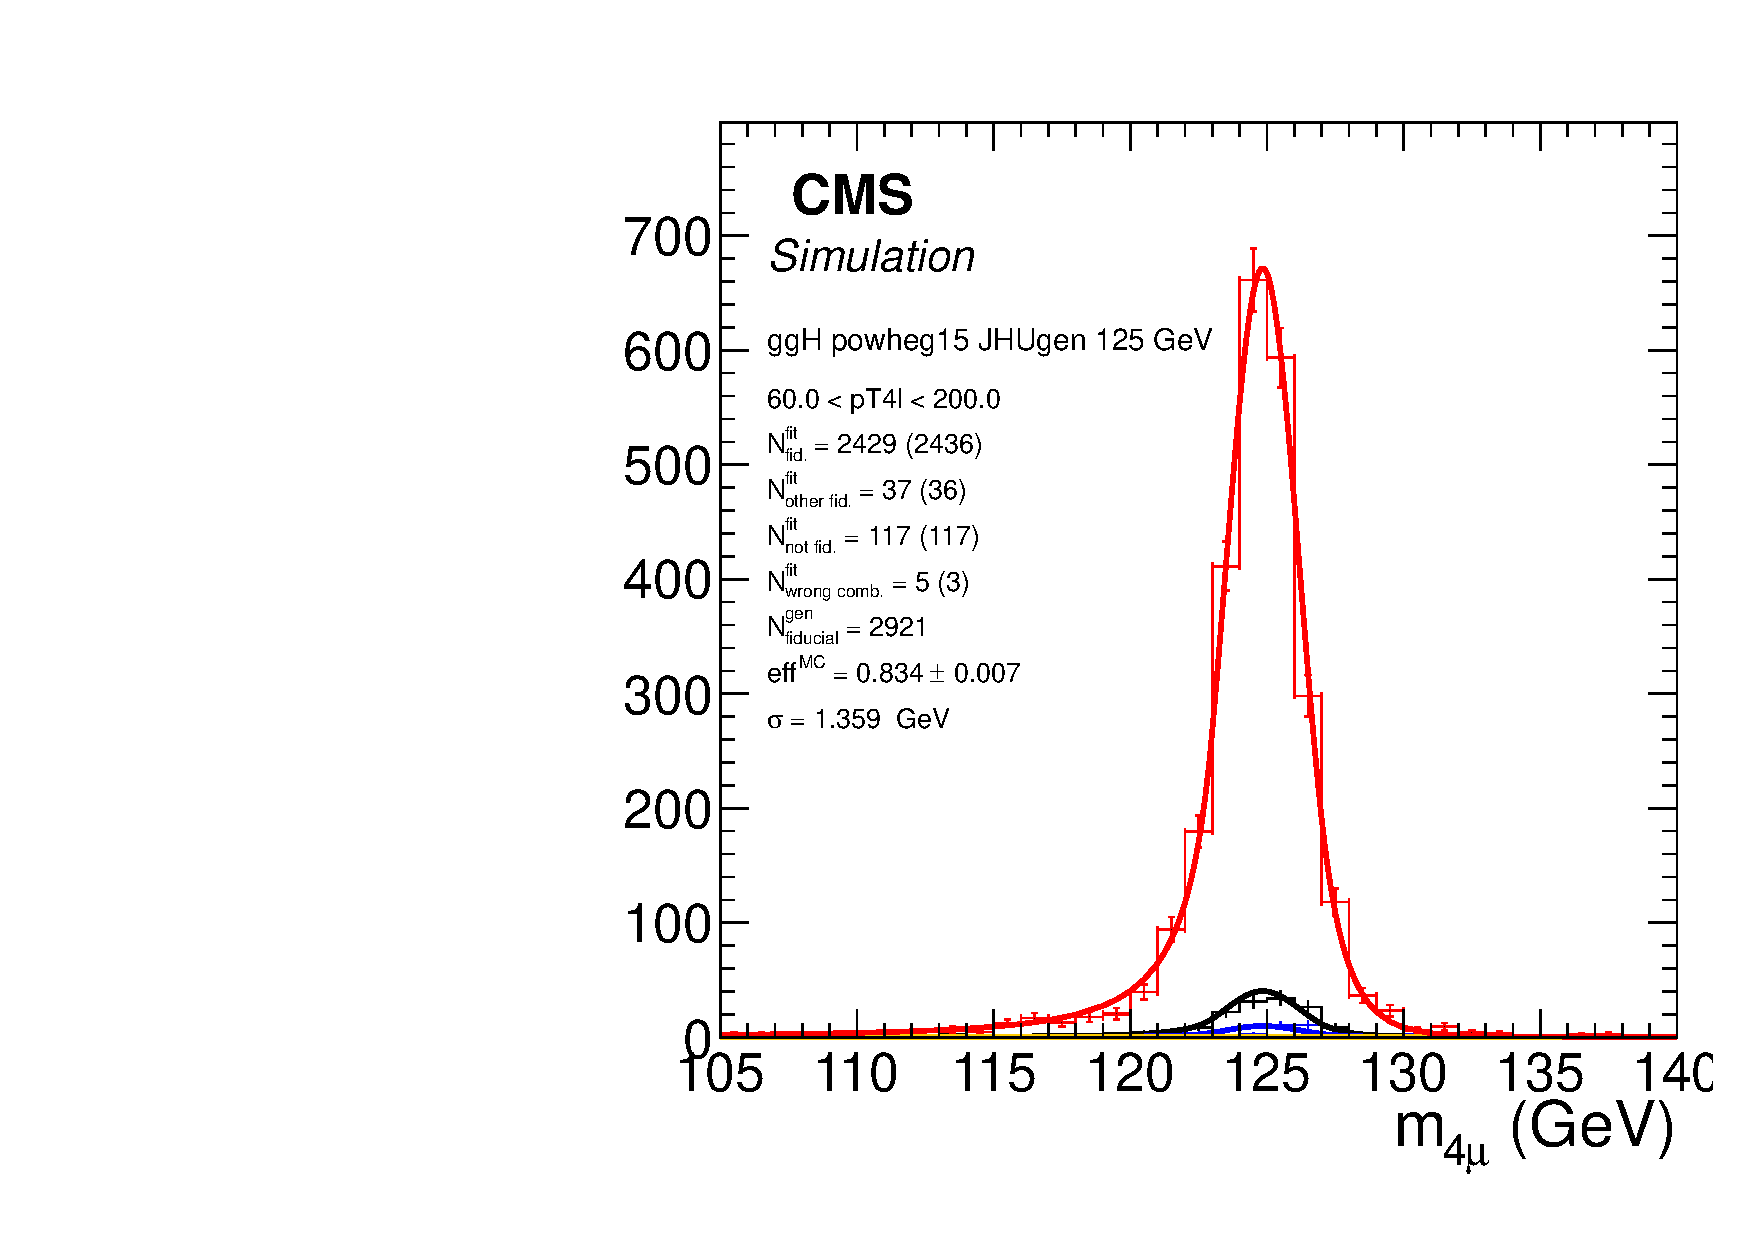
\includegraphics[width=0.3\textwidth,angle=0]{Figures/results/fiducial/2018//ggH_powheg15_JHUgen_125_4mu_pT4l_genbin3_recobin3_effs_eventMCWeight.pdf}
%      \label{fig:sigfits-pT4l-ggH-powheg15-JHUgen-125-maintext:k}
%    }
%    \subfigure[$60.0  < \pt(\mathrm{H}) < 200.0$]{
%      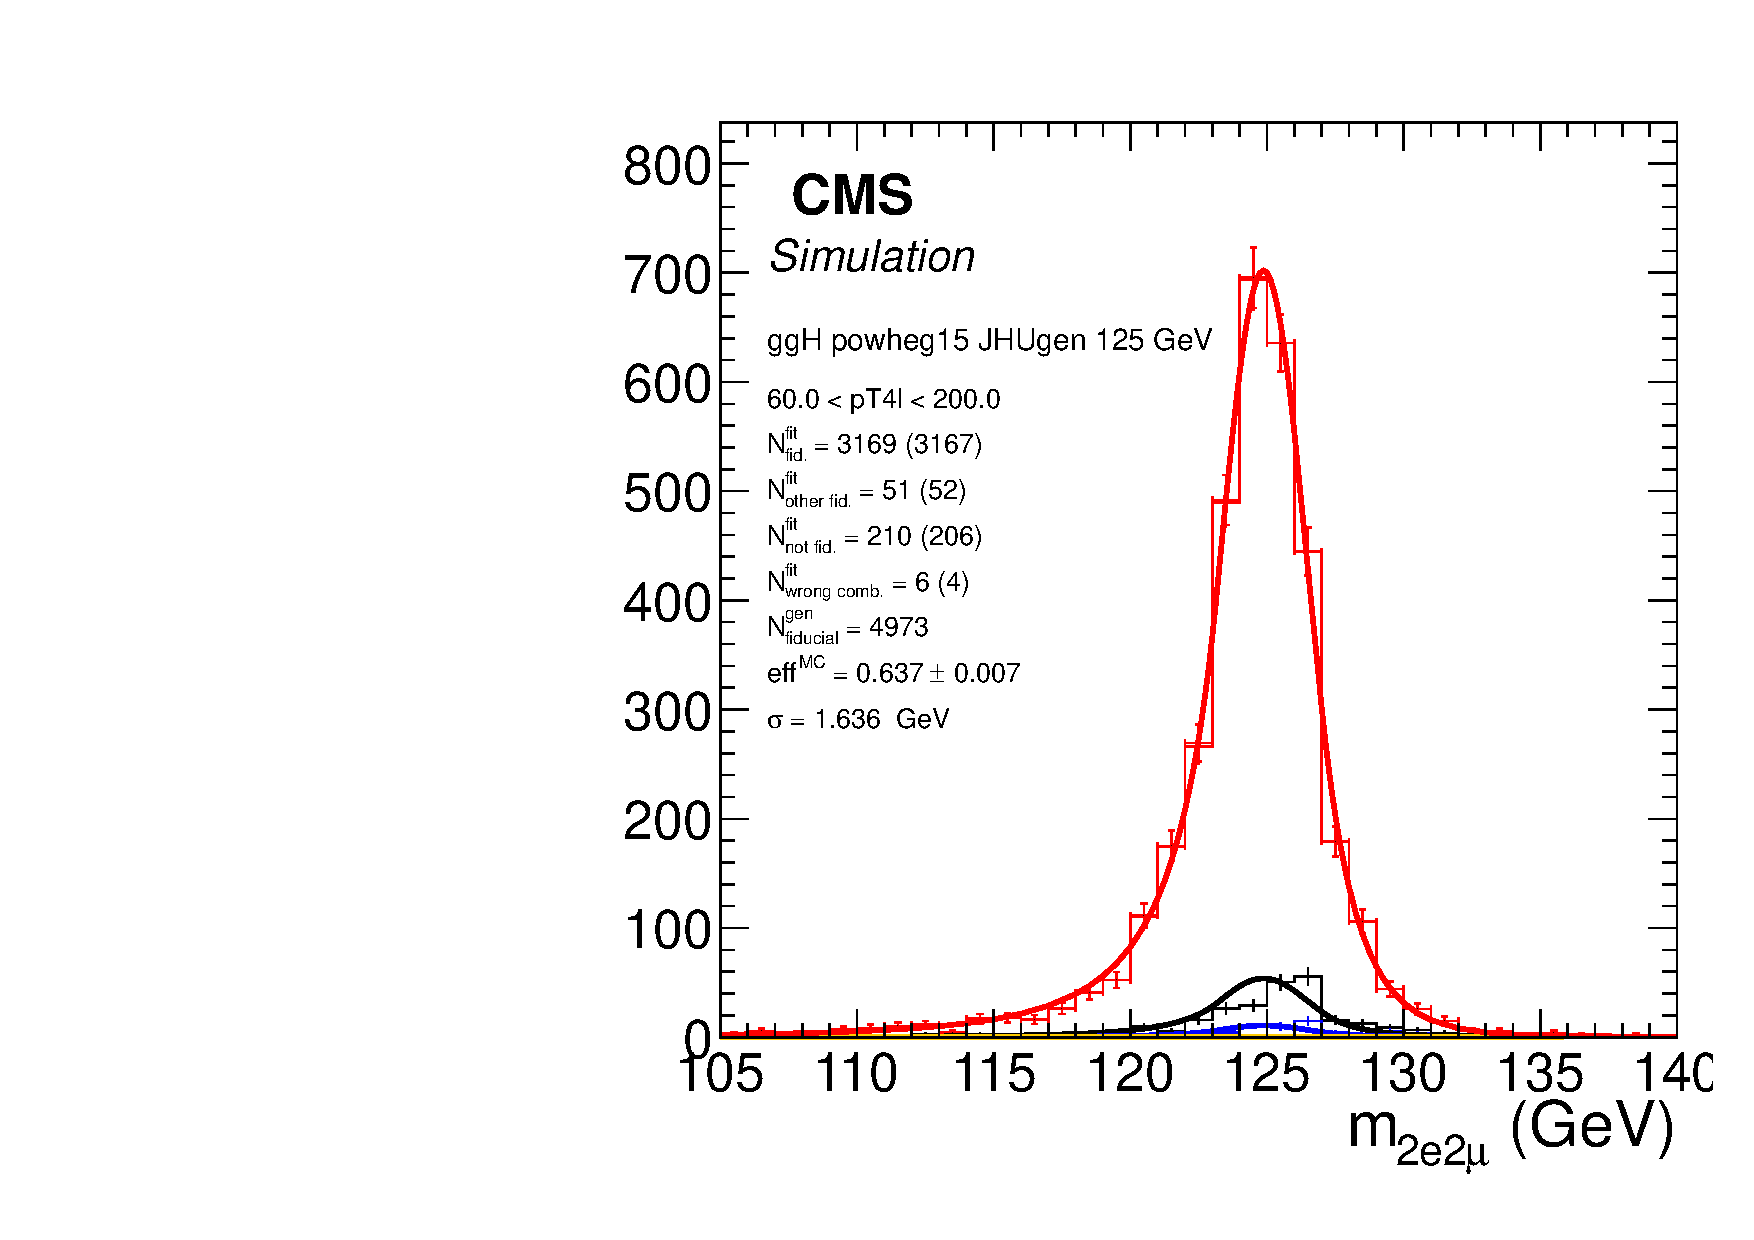
\includegraphics[width=0.3\textwidth,angle=0]{Figures/results/fiducial/2018//ggH_powheg15_JHUgen_125_2e2mu_pT4l_genbin3_recobin3_effs_eventMCWeight.pdf}
%      \label{fig:sigfits-pT4l-ggH-powheg15-JHUgen-125-maintext:l}
%    }
    \\
    \caption{ Example signal shapes at reconstruction level for a resonance of m(4$\ell$) in $2e2\mu$ final state for the $gg\rightarrow \mathrm{H}$ production mode from {\sc powheg+JHUGen} in different bins of $\pt(\mathrm{H})$. The black curve represents events which do not pass the fiducial volume selection. The curve has no effect on the result.
    }
  \label{fig:sigfits-pT4l-ggH-powheg15-JHUgen-125-maintext}
 \end{center}
\end{figure} \clearpage

%%%%%%%%%5
\begin{figure}[htb]
  \begin{center}
    \subfigure[$gg\rightarrow$H ({\sc powheg+JHUgen})]{
    %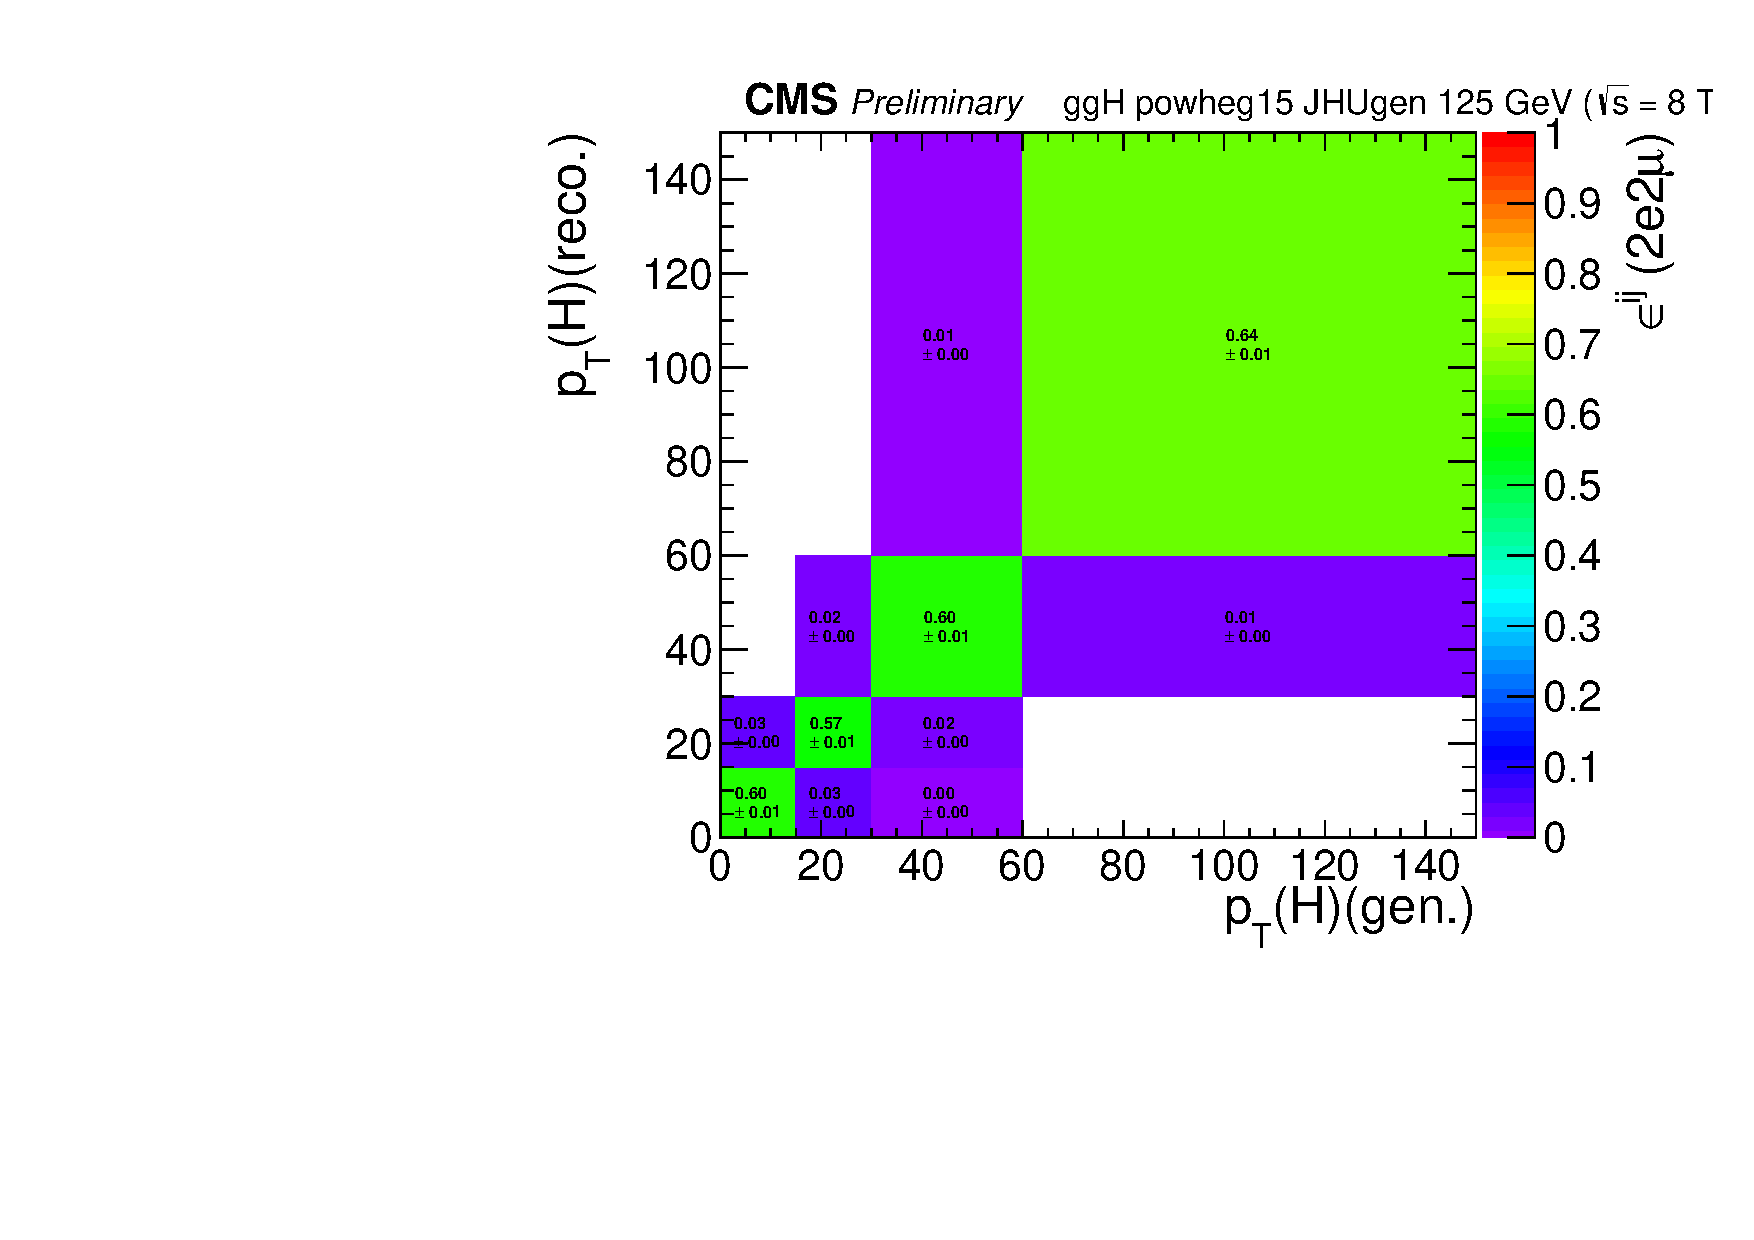
\includegraphics[width=0.48\textwidth,angle=0]{Figures/results/fiducial/2018//eff2d_ggH_powheg15_JHUgen_125_pT4l_2e2mu.pdf}
    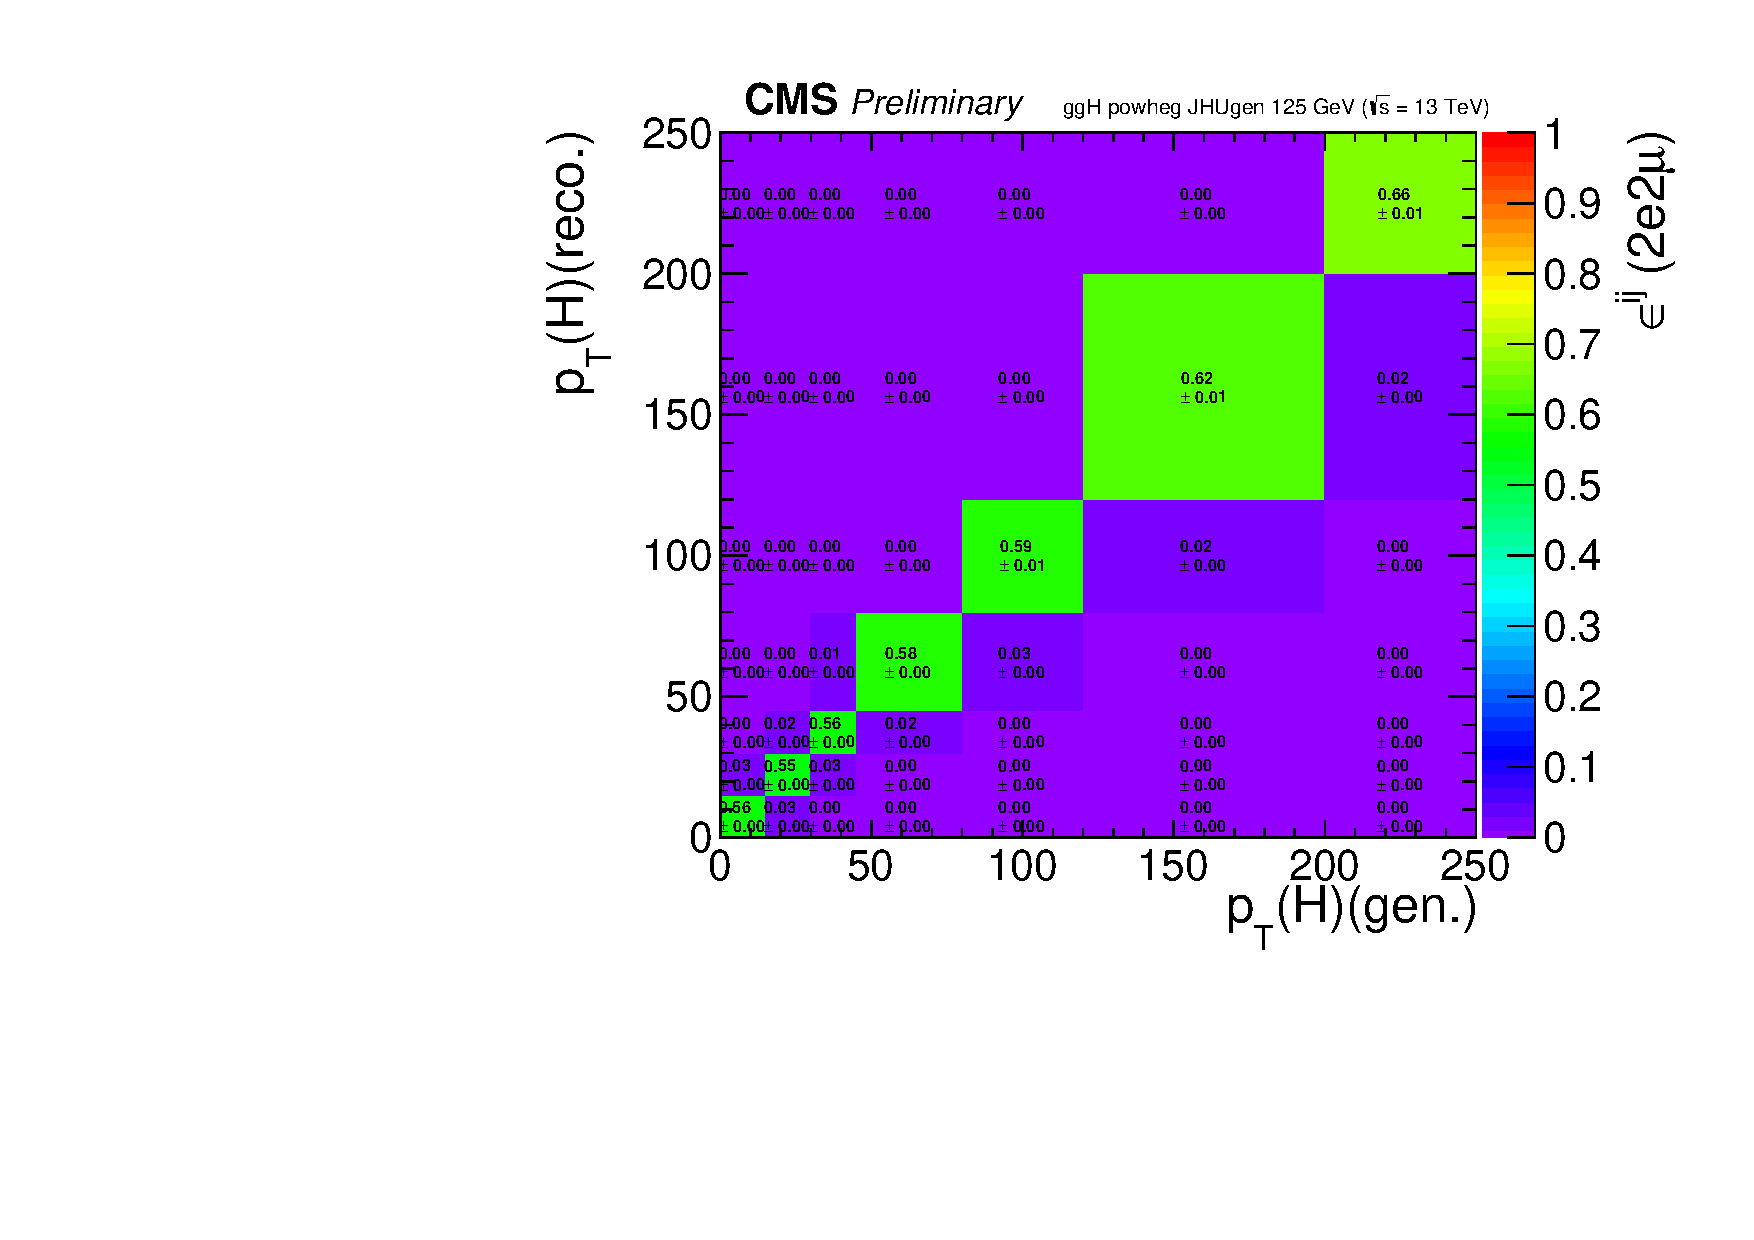
\includegraphics[width=0.48\textwidth,angle=0]{Figures/results/fiducial/2018//eff2d_ggH_powheg_JHUgen_125_pT4l_2e2mu.pdf}
    \label{fig:eff-pT4l-2e2mu-maintext:a}
    }
    \subfigure[$gg\rightarrow$H ({\sc minloHJJ})]{
    %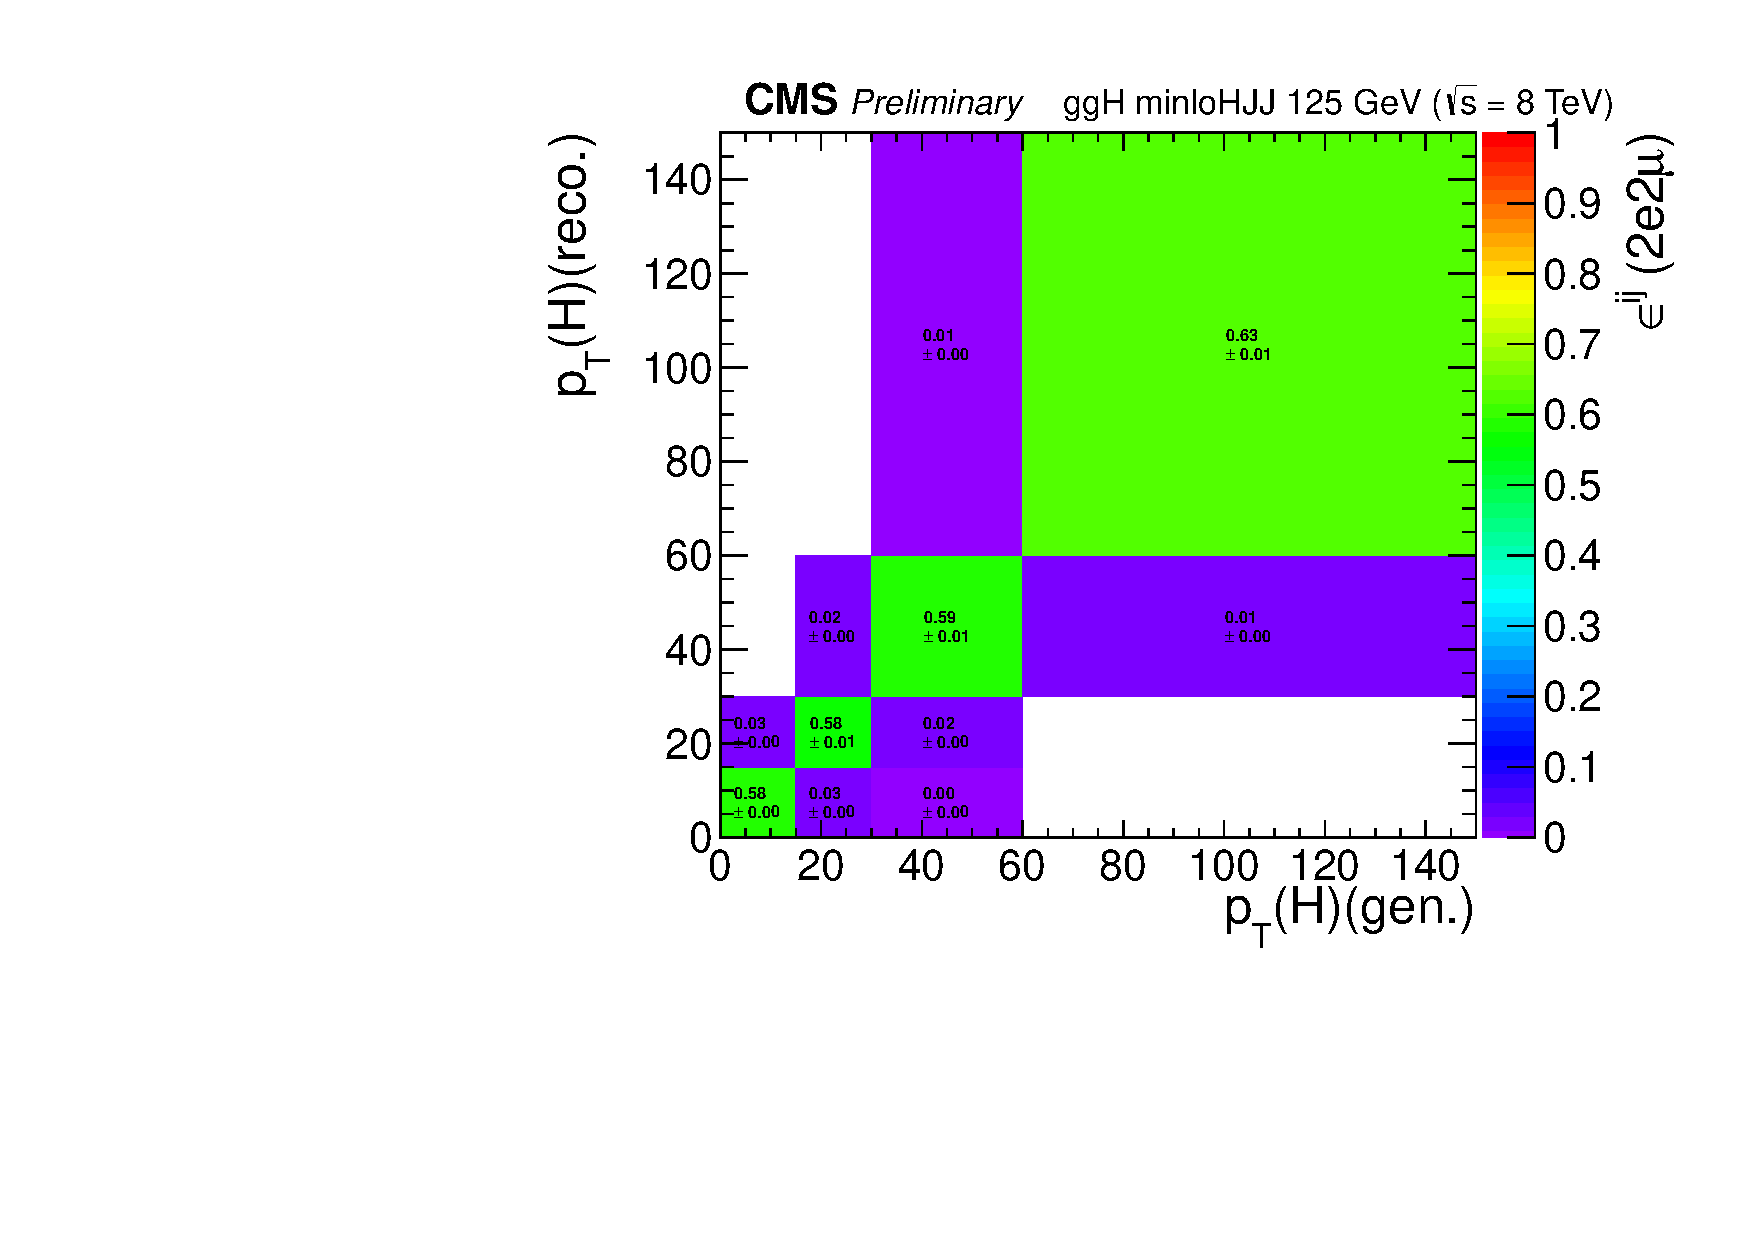
\includegraphics[width=0.48\textwidth,angle=0]{Figures/results/fiducial/2018//eff2d_ggH_minloHJJ_125_pT4l_2e2mu.pdf}
    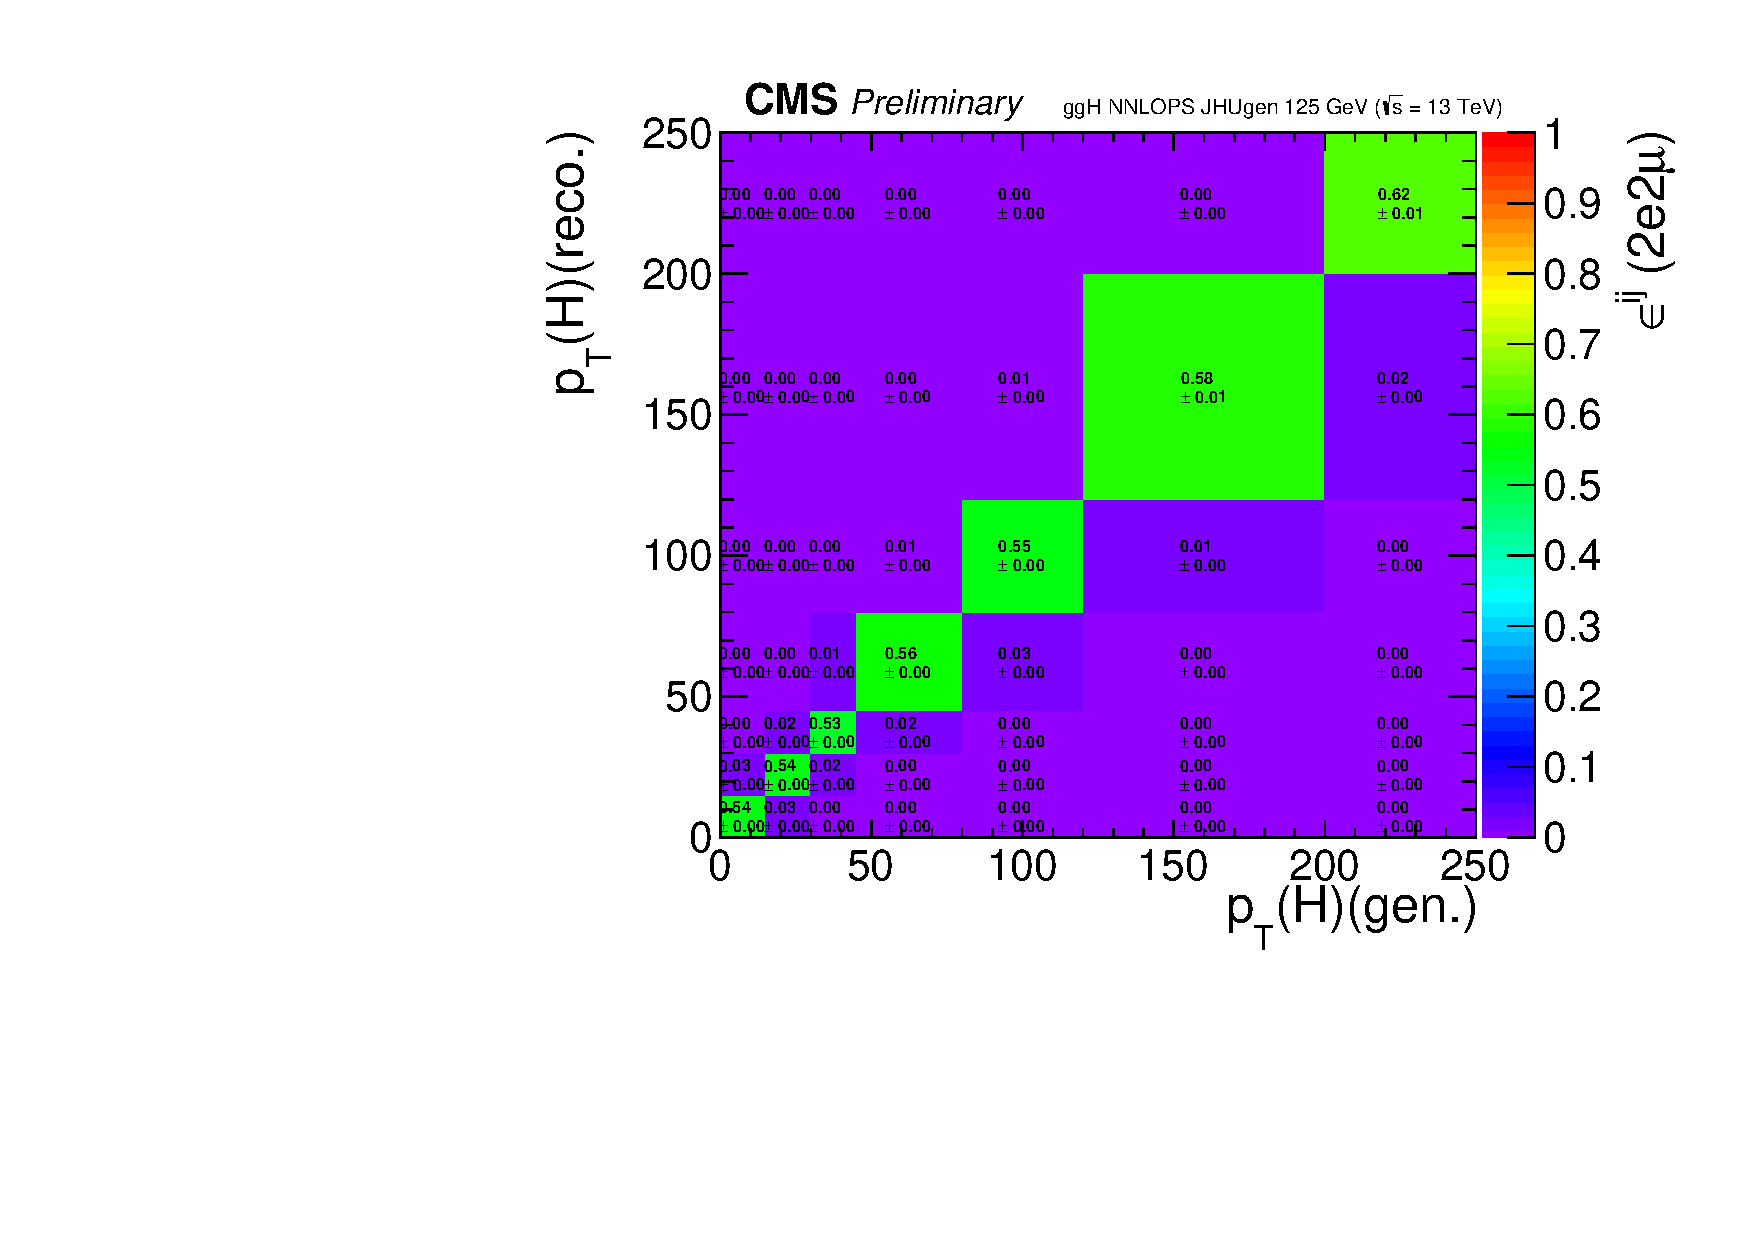
\includegraphics[width=0.48\textwidth,angle=0]{Figures/results/fiducial/2018//eff2d_ggH_NNLOPS_JHUgen_125_pT4l_2e2mu.pdf}
    \label{fig:eff-pT4l-2e2mu-maintext:b}
    } \\
    \subfigure[VBF ({\sc powheg})]{
    %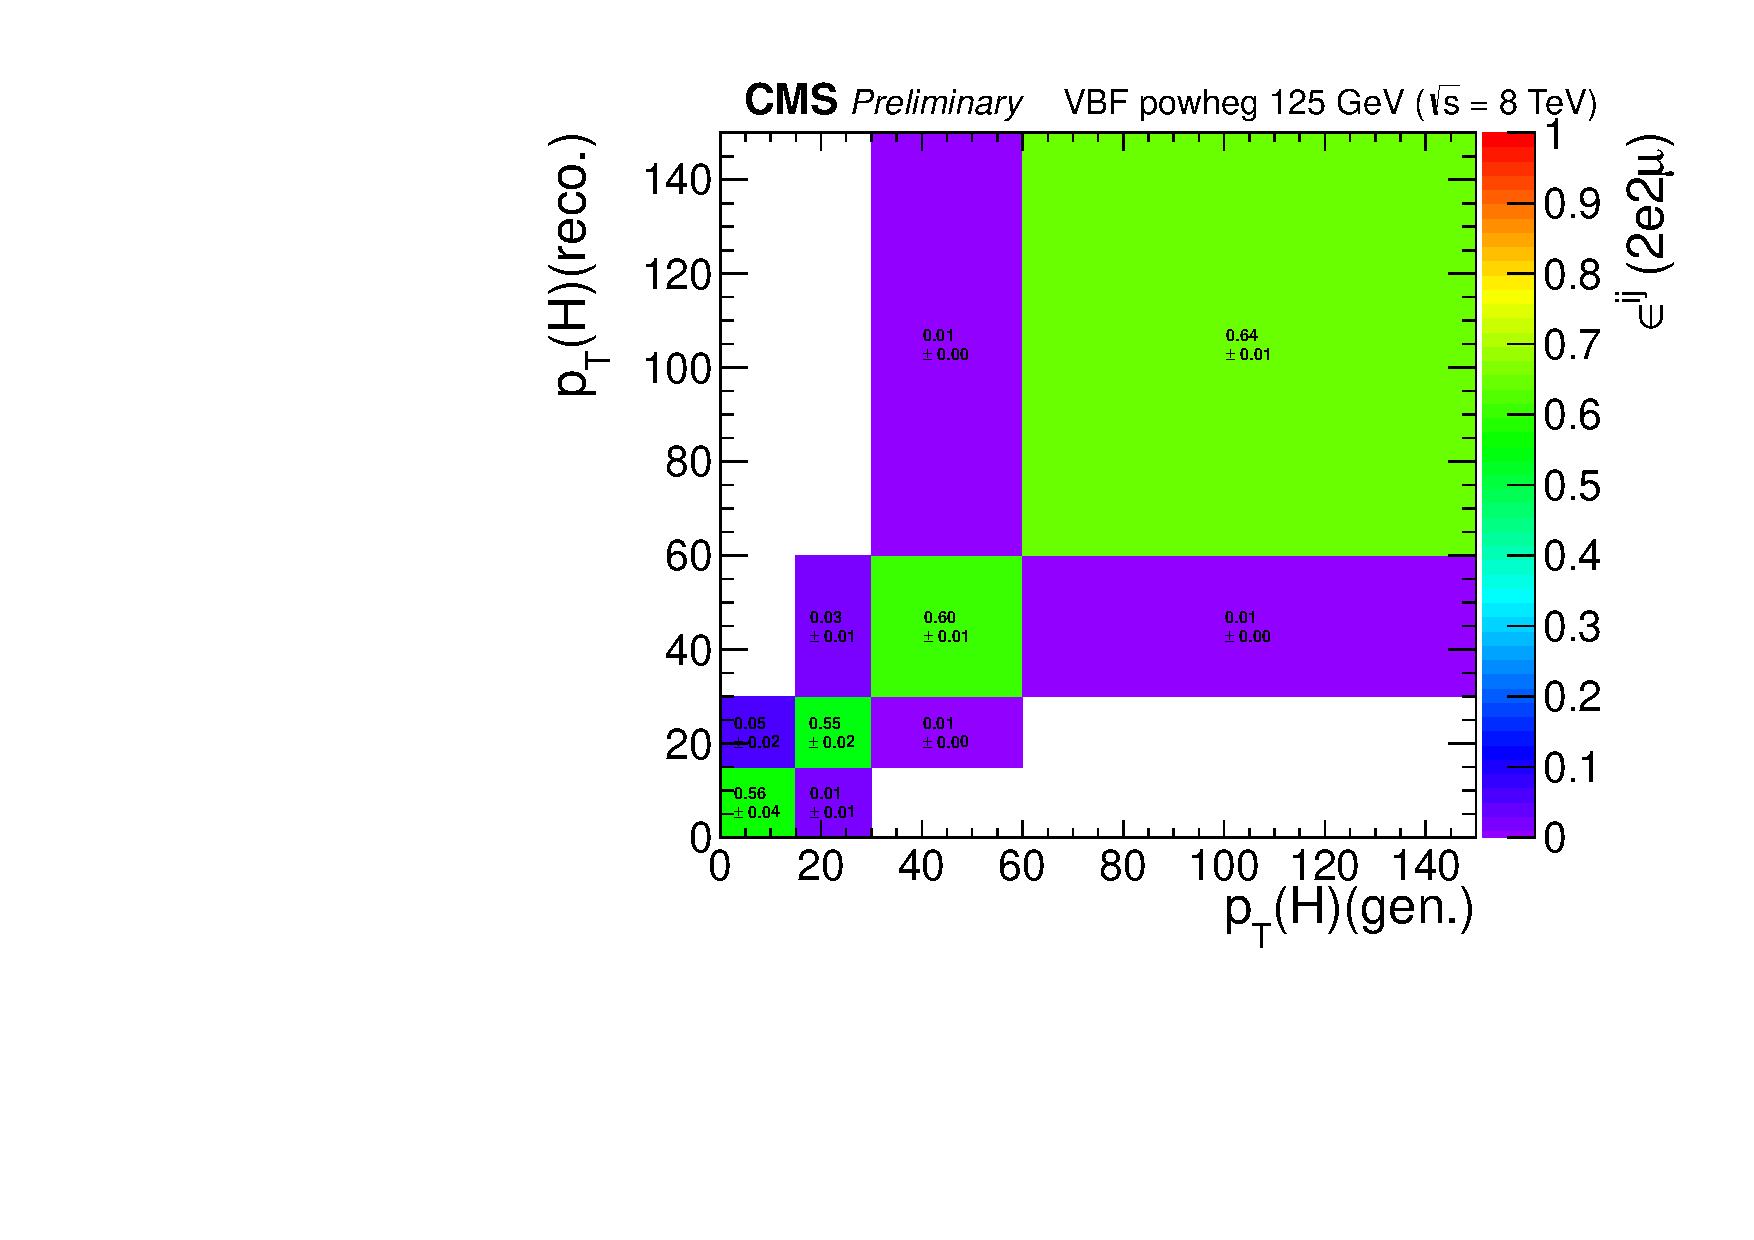
\includegraphics[width=0.48\textwidth,angle=0]{Figures/results/fiducial/2018//eff2d_VBF_powheg_125_pT4l_2e2mu.pdf}
    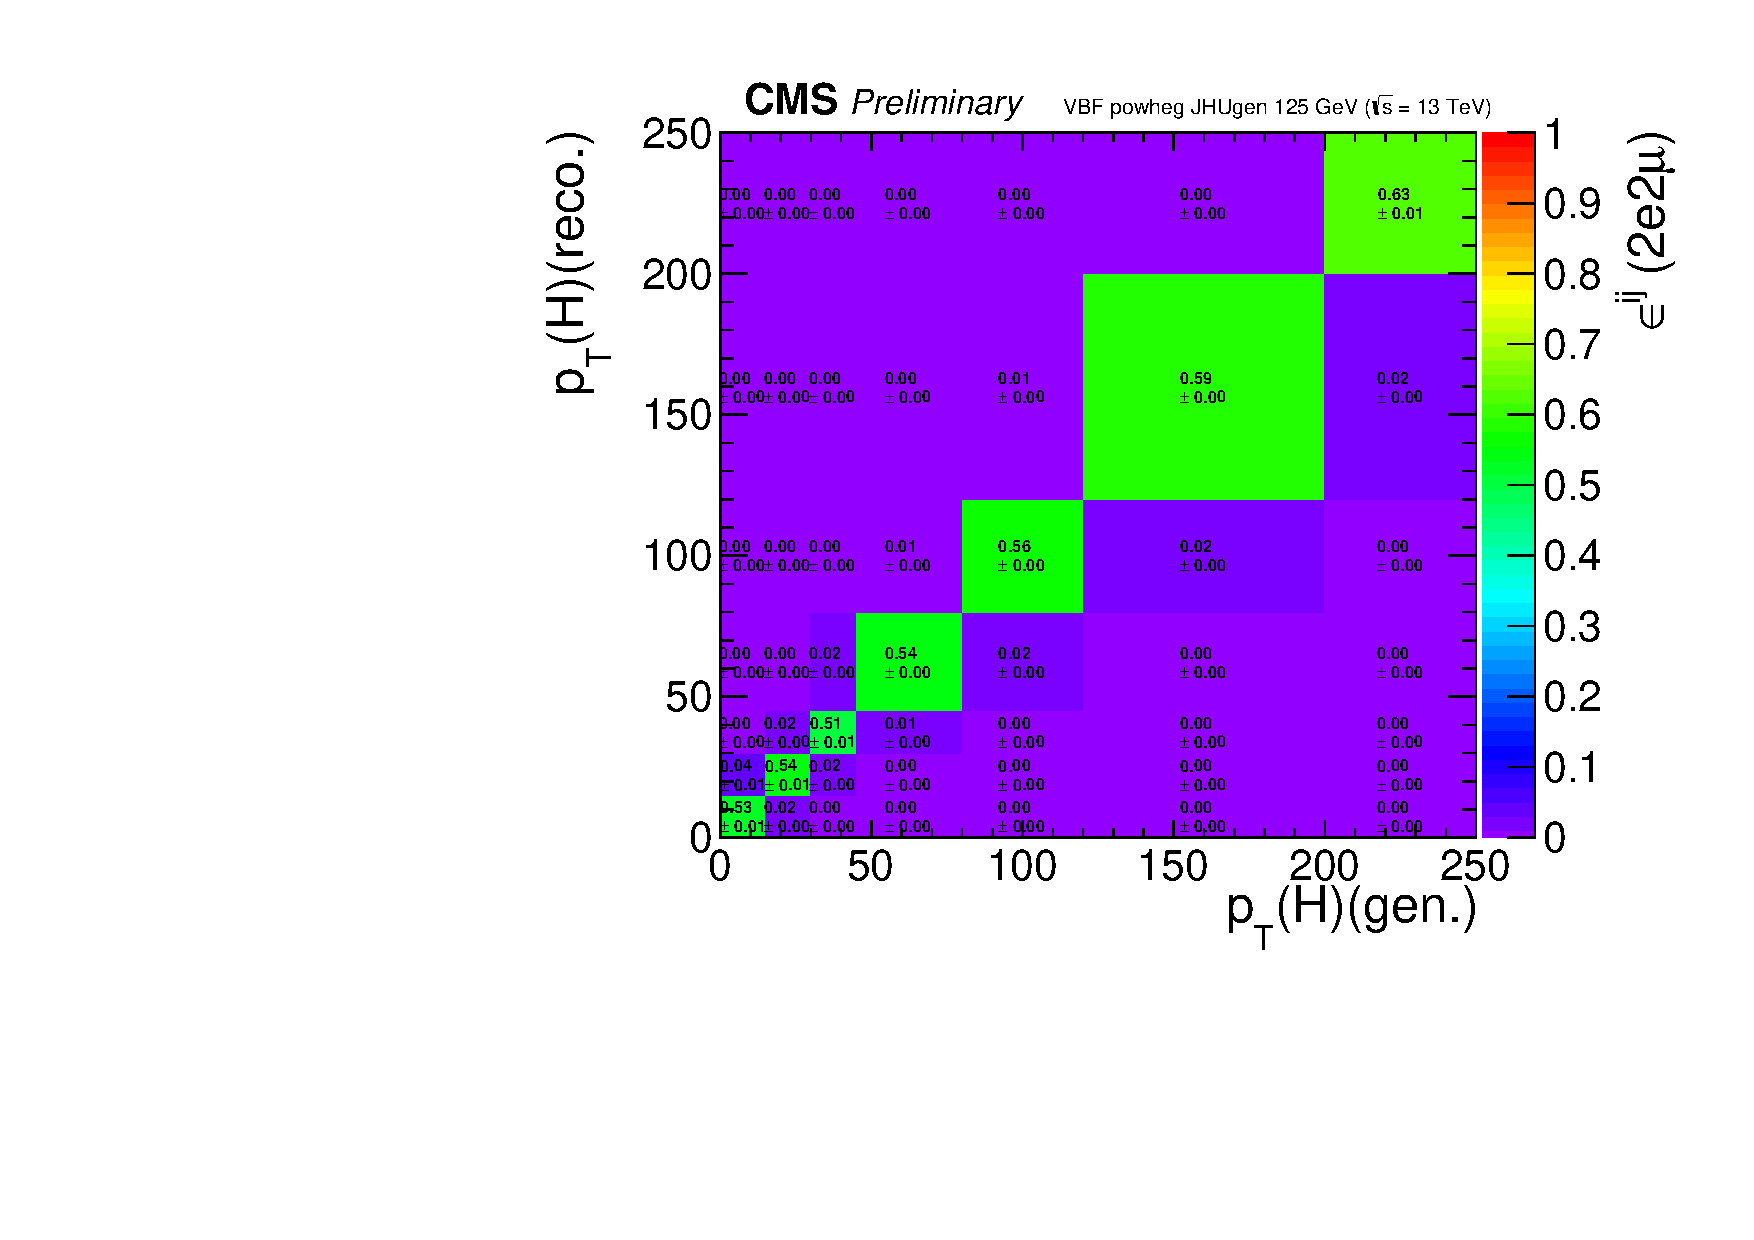
\includegraphics[width=0.48\textwidth,angle=0]{Figures/results/fiducial/2018//eff2d_VBF_powheg_JHUgen_125_pT4l_2e2mu.pdf}
    \label{fig:eff-pT4l-2e2mu-maintext:c}
    }
    \subfigure[WH ({\sc pythia})]{
    %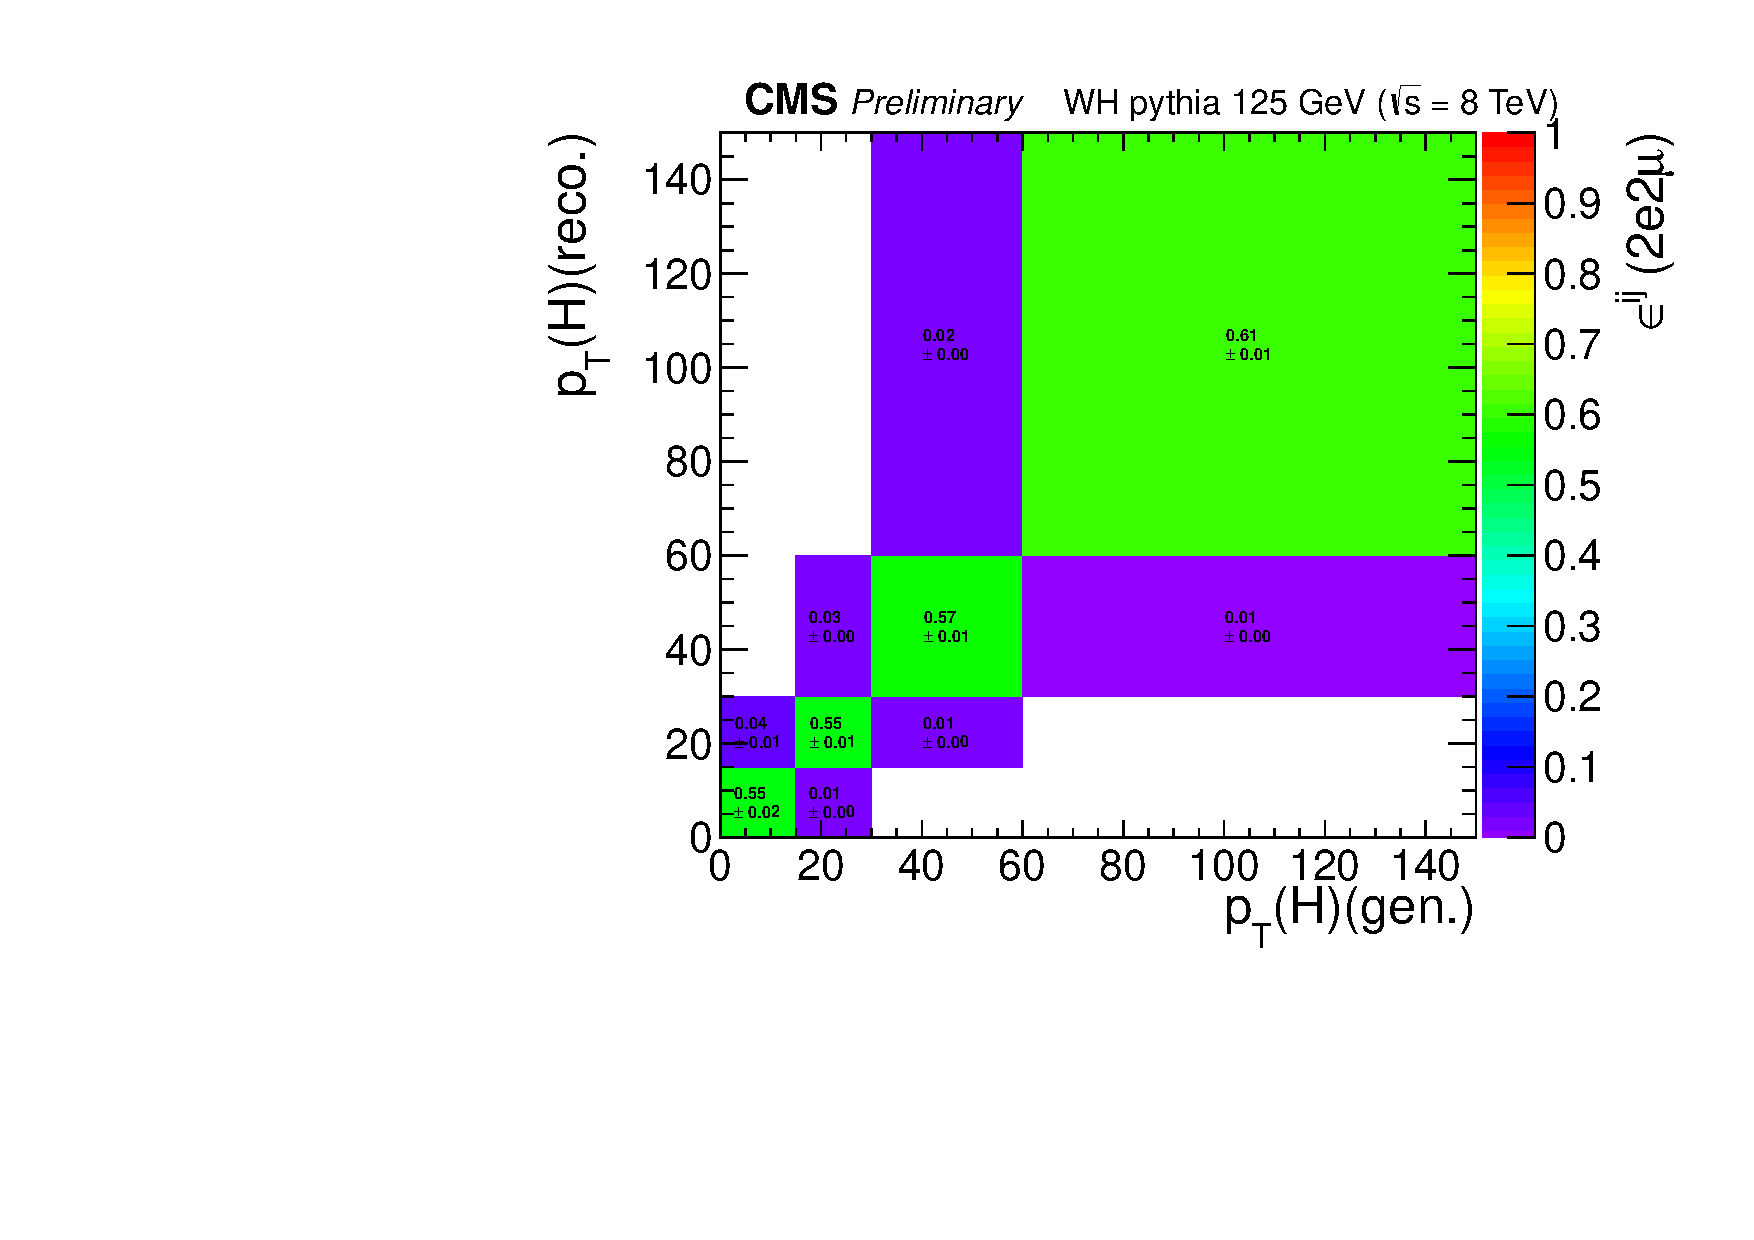
\includegraphics[width=0.48\textwidth,angle=0]{Figures/results/fiducial/2018//eff2d_WH_pythia_125_pT4l_2e2mu.pdf}
    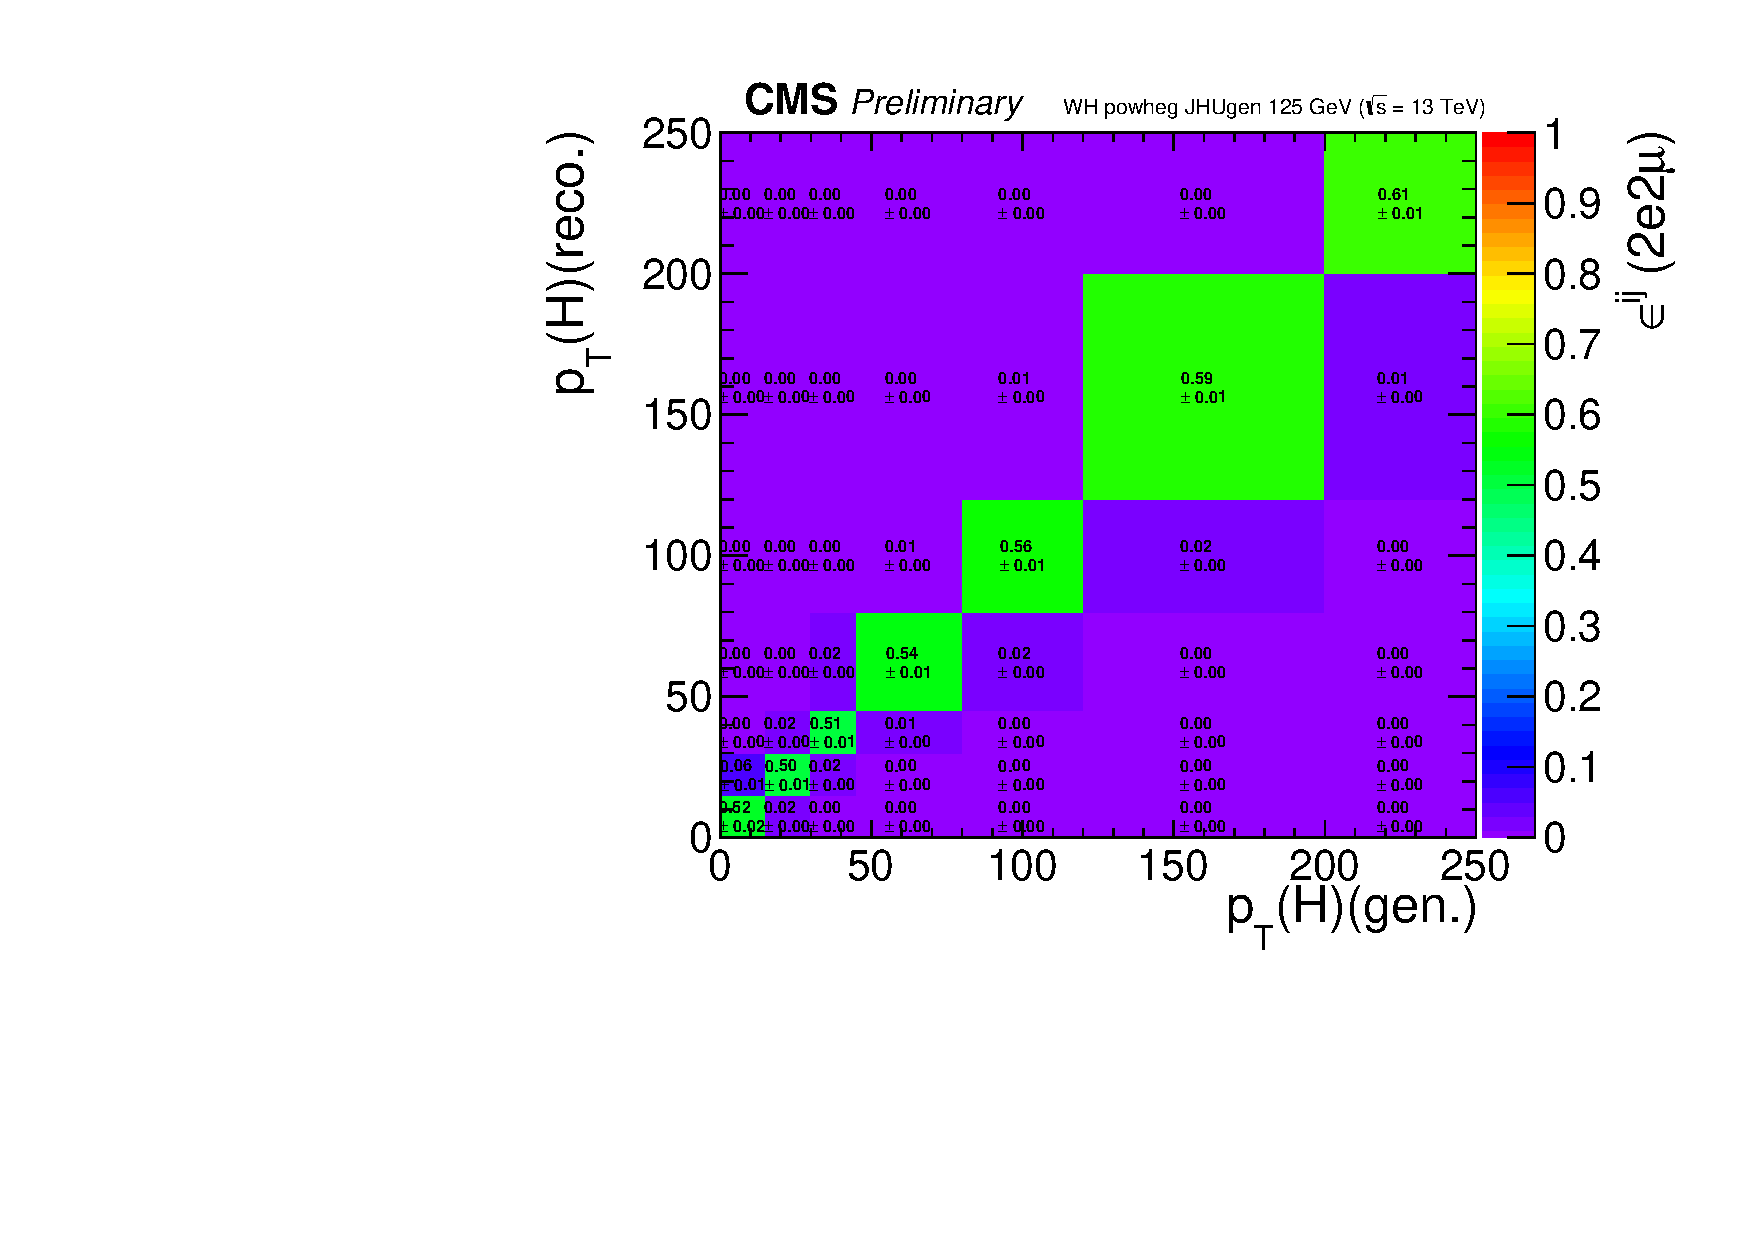
\includegraphics[width=0.48\textwidth,angle=0]{Figures/results/fiducial/2018//eff2d_WH_powheg_JHUgen_125_pT4l_2e2mu.pdf}
    \label{fig:eff-pT4l-2e2mu-maintext:d}
    } \\
    \subfigure[ZH ({\sc pythia})]{
    %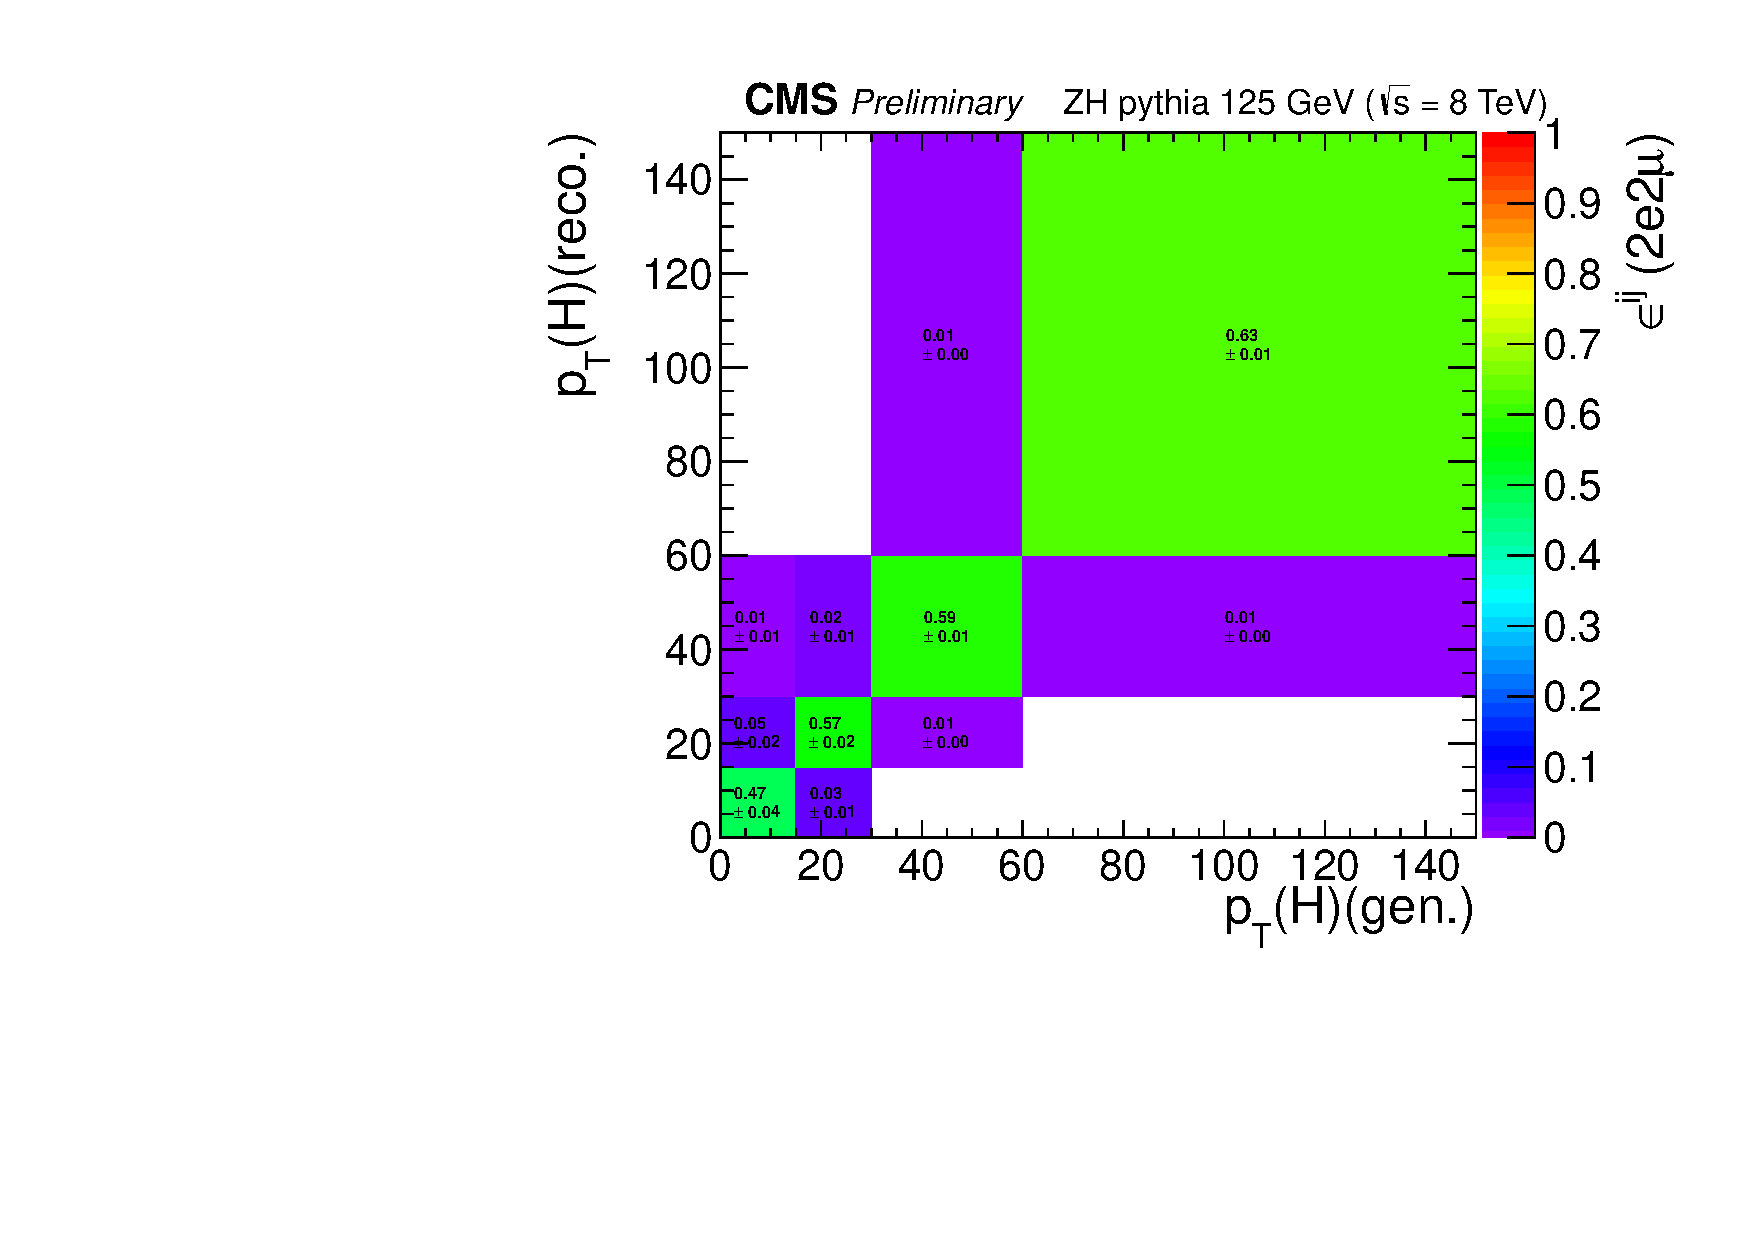
\includegraphics[width=0.48\textwidth,angle=0]{Figures/results/fiducial/2018//eff2d_ZH_pythia_125_pT4l_2e2mu.pdf}
    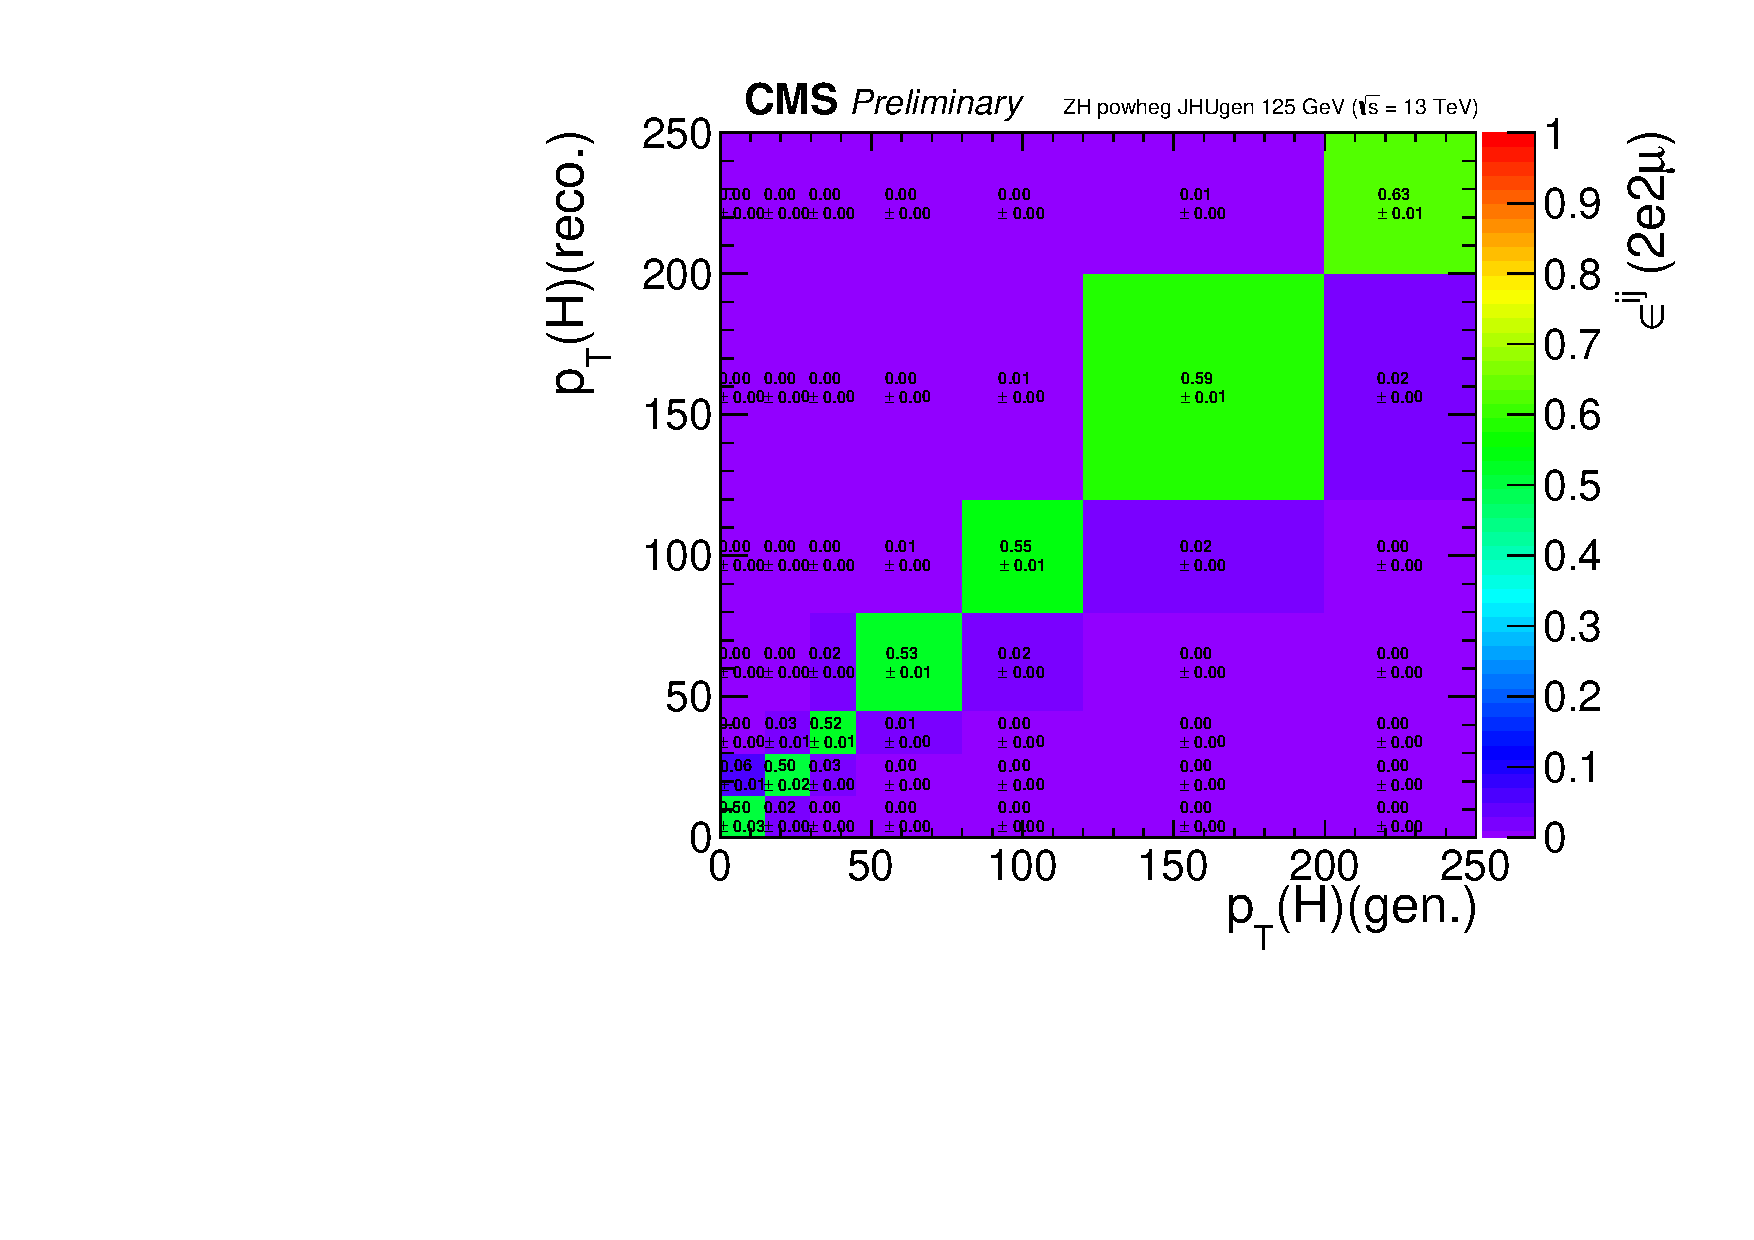
\includegraphics[width=0.48\textwidth,angle=0]{Figures/results/fiducial/2018//eff2d_ZH_powheg_JHUgen_125_pT4l_2e2mu.pdf}
    \label{fig:eff-pT4l-2e2mu-maintext:e}
    }
    \subfigure[ttH ({\sc pythia})]{
    %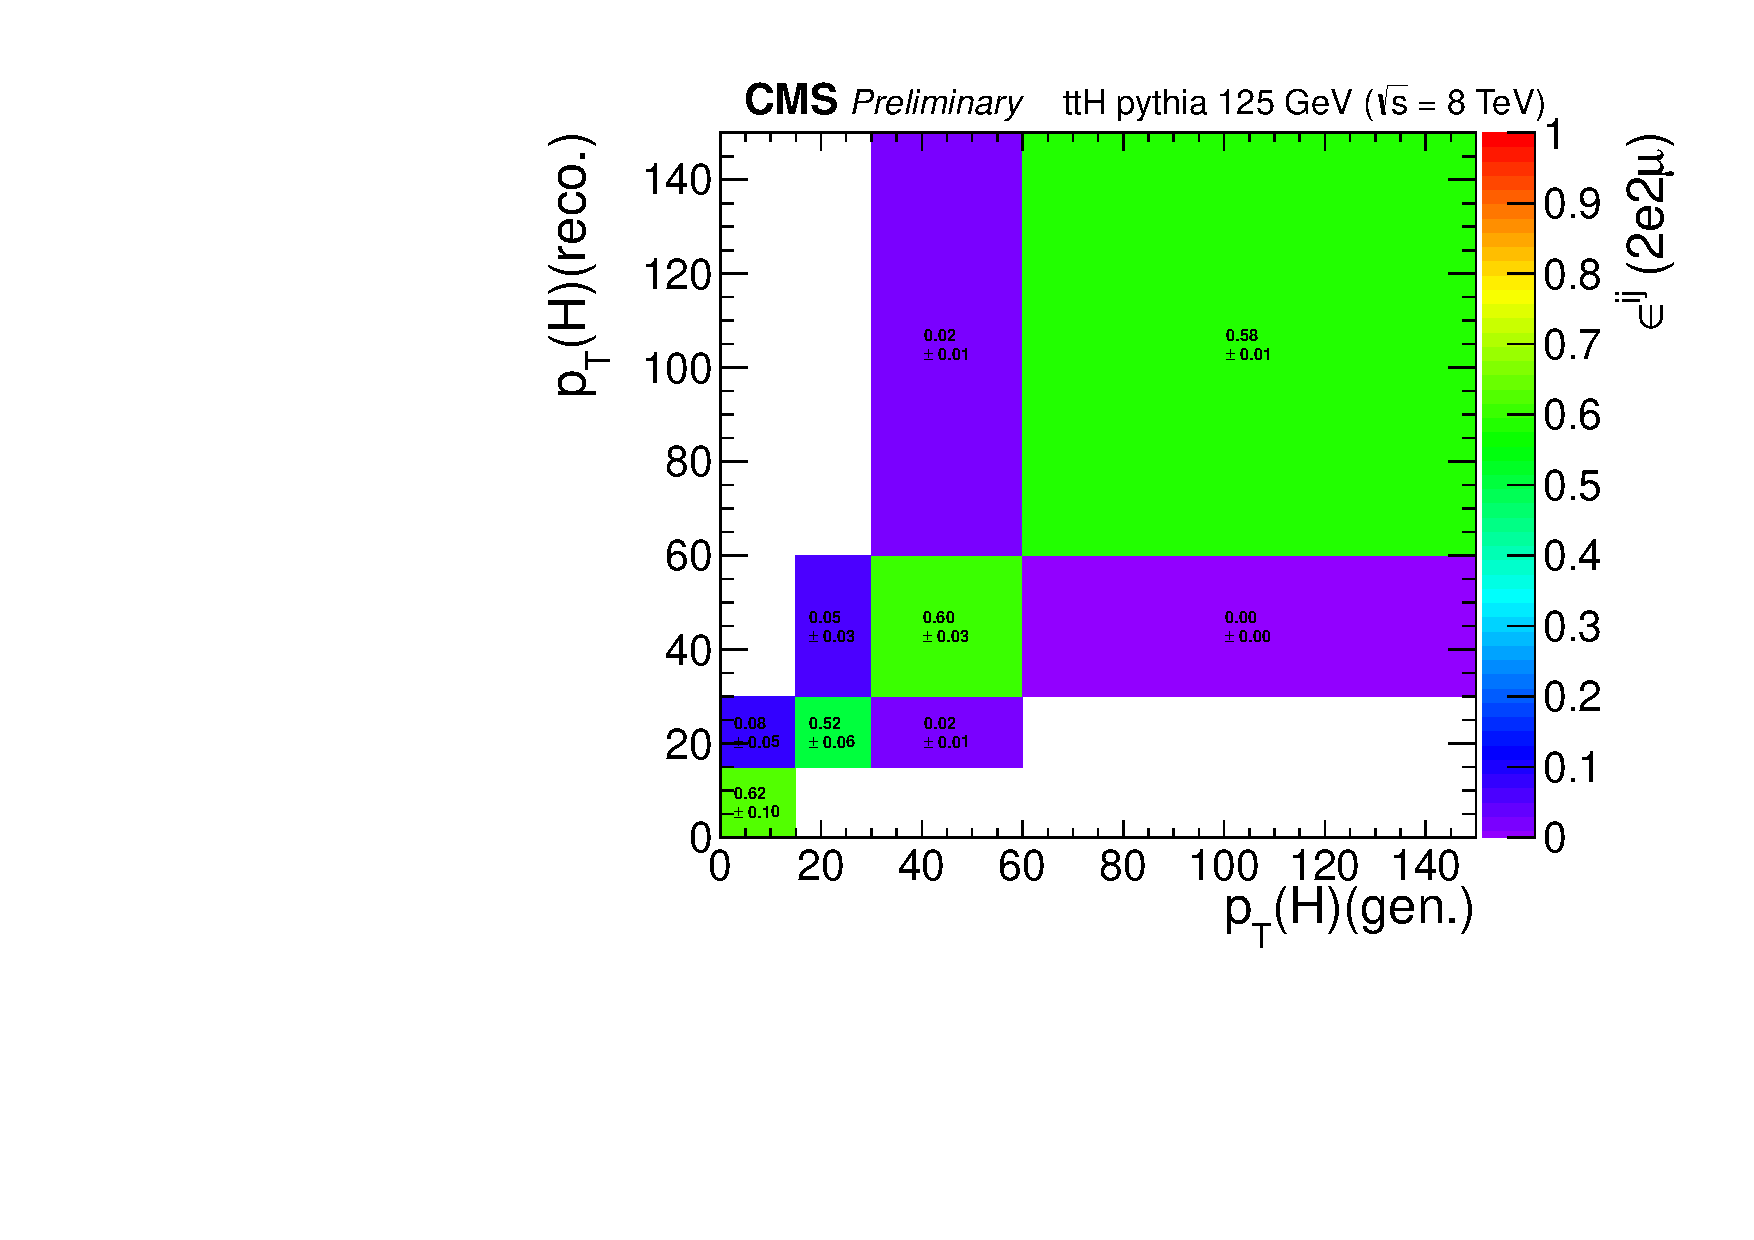
\includegraphics[width=0.48\textwidth,angle=0]{Figures/results/fiducial/2018//eff2d_ttH_pythia_125_pT4l_2e2mu.pdf}
    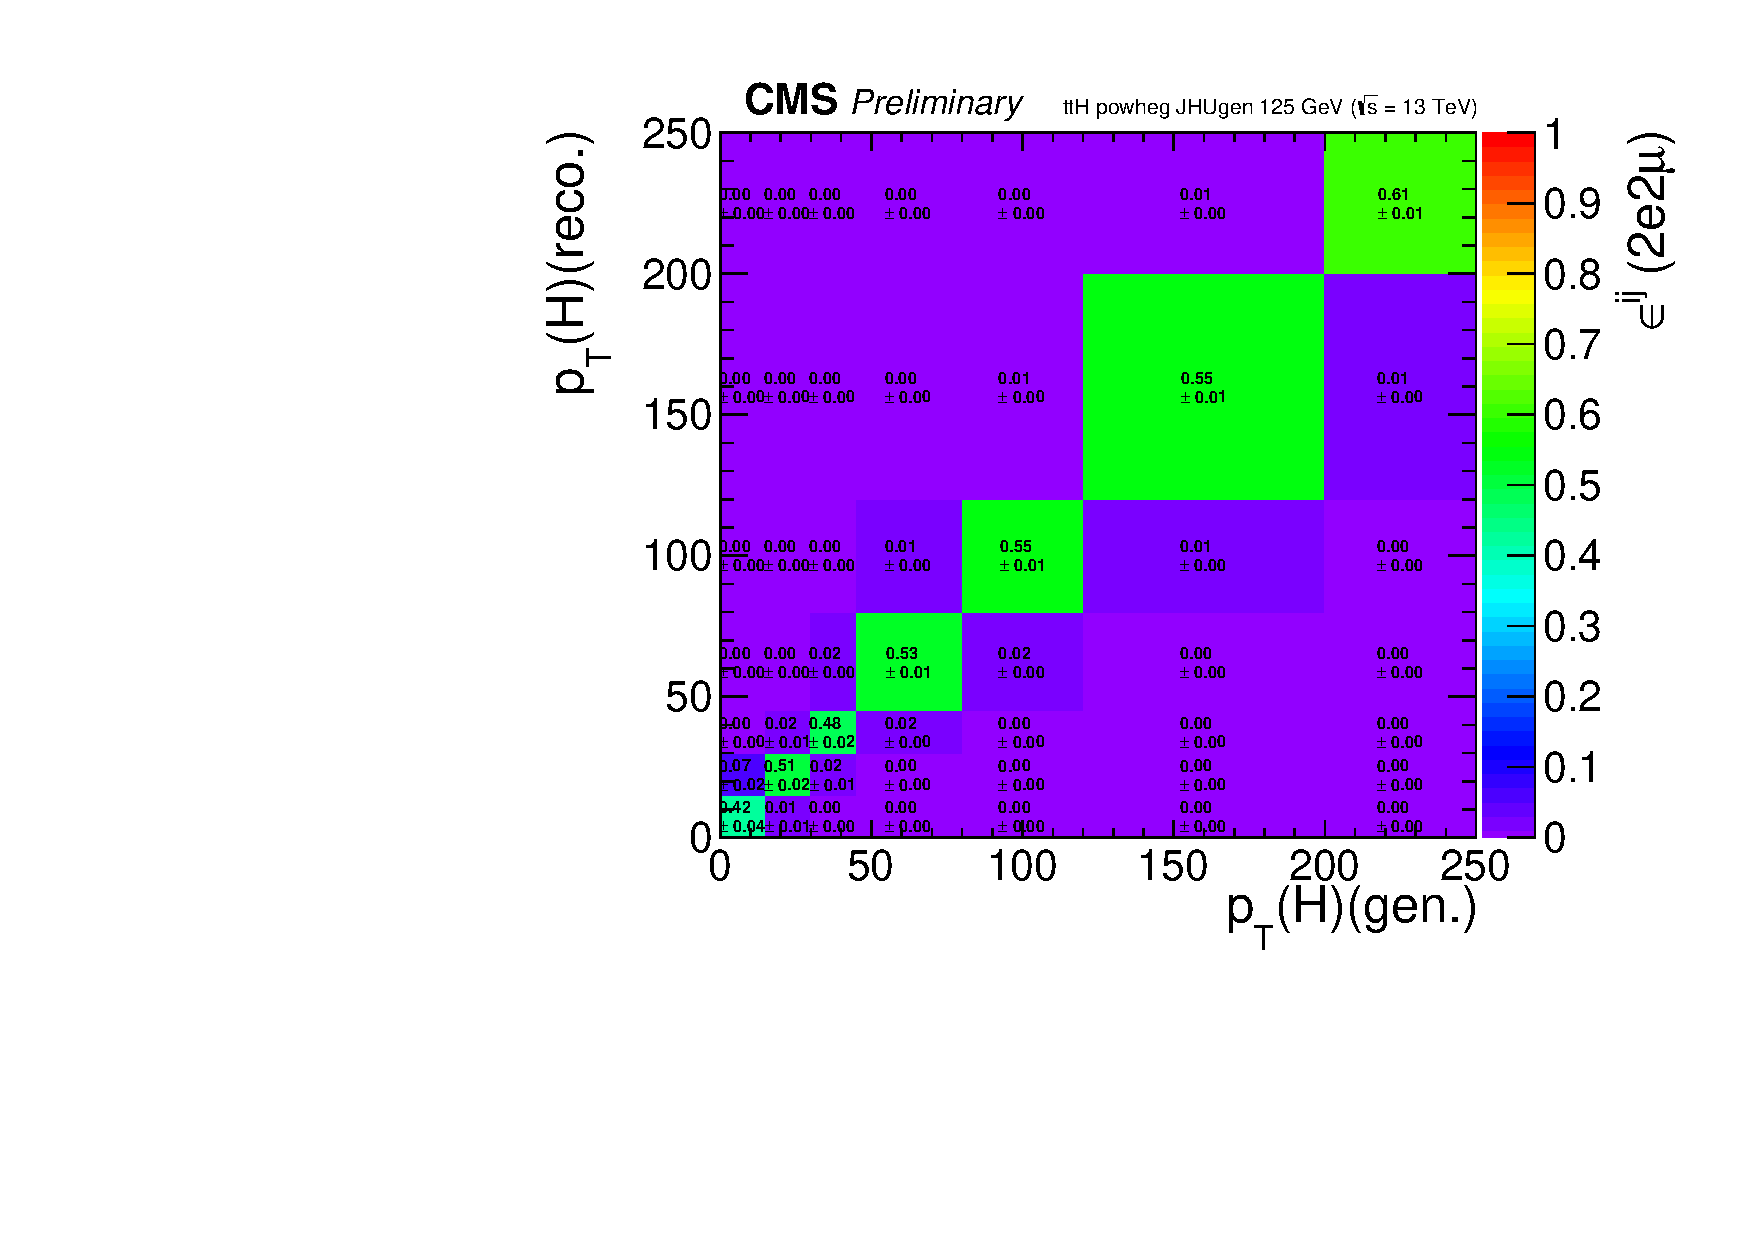
\includegraphics[width=0.48\textwidth,angle=0]{Figures/results/fiducial/2018//eff2d_ttH_powheg_JHUgen_125_pT4l_2e2mu.pdf}
    \label{fig:eff-pT4l-2e2mu-maintext:f}
    }
    \caption{ Efficiency response matrices for $\pt({\rm H})$ for different SM production modes in the $2e2\mu$ final state using 2018 samples. }
    \label{fig:eff-pT4l-2e2mu-maintext}
  \end{center}
\end{figure} \clearpage
%%%%%%%
%Figure~\ref{fig:sigfits-asimov-SM-pt4l-4l} shows the four lepton mass distributions for an Asimov dataset generated using SM cross section values and efficiencies 
%from the gg$\rightarrow$H production mode from {\sc powheg+JHUgen}, and resulting fitted values of PDFs of signal and background for different bins of $\pt(\mathrm{H})$ (all final states combined).
%The same distributions and resulting fitted values of the signal and background pdfs in bins of all considered observables can be found in the Appendix~\ref{}.
% |0|15|30|45|80|120|200|13000|
\begin{figure}[htb]
  \begin{center}
    \subfigure[$0.0 \GeV < \pt(\mathrm{H}) < 15.0 \GeV$]{
      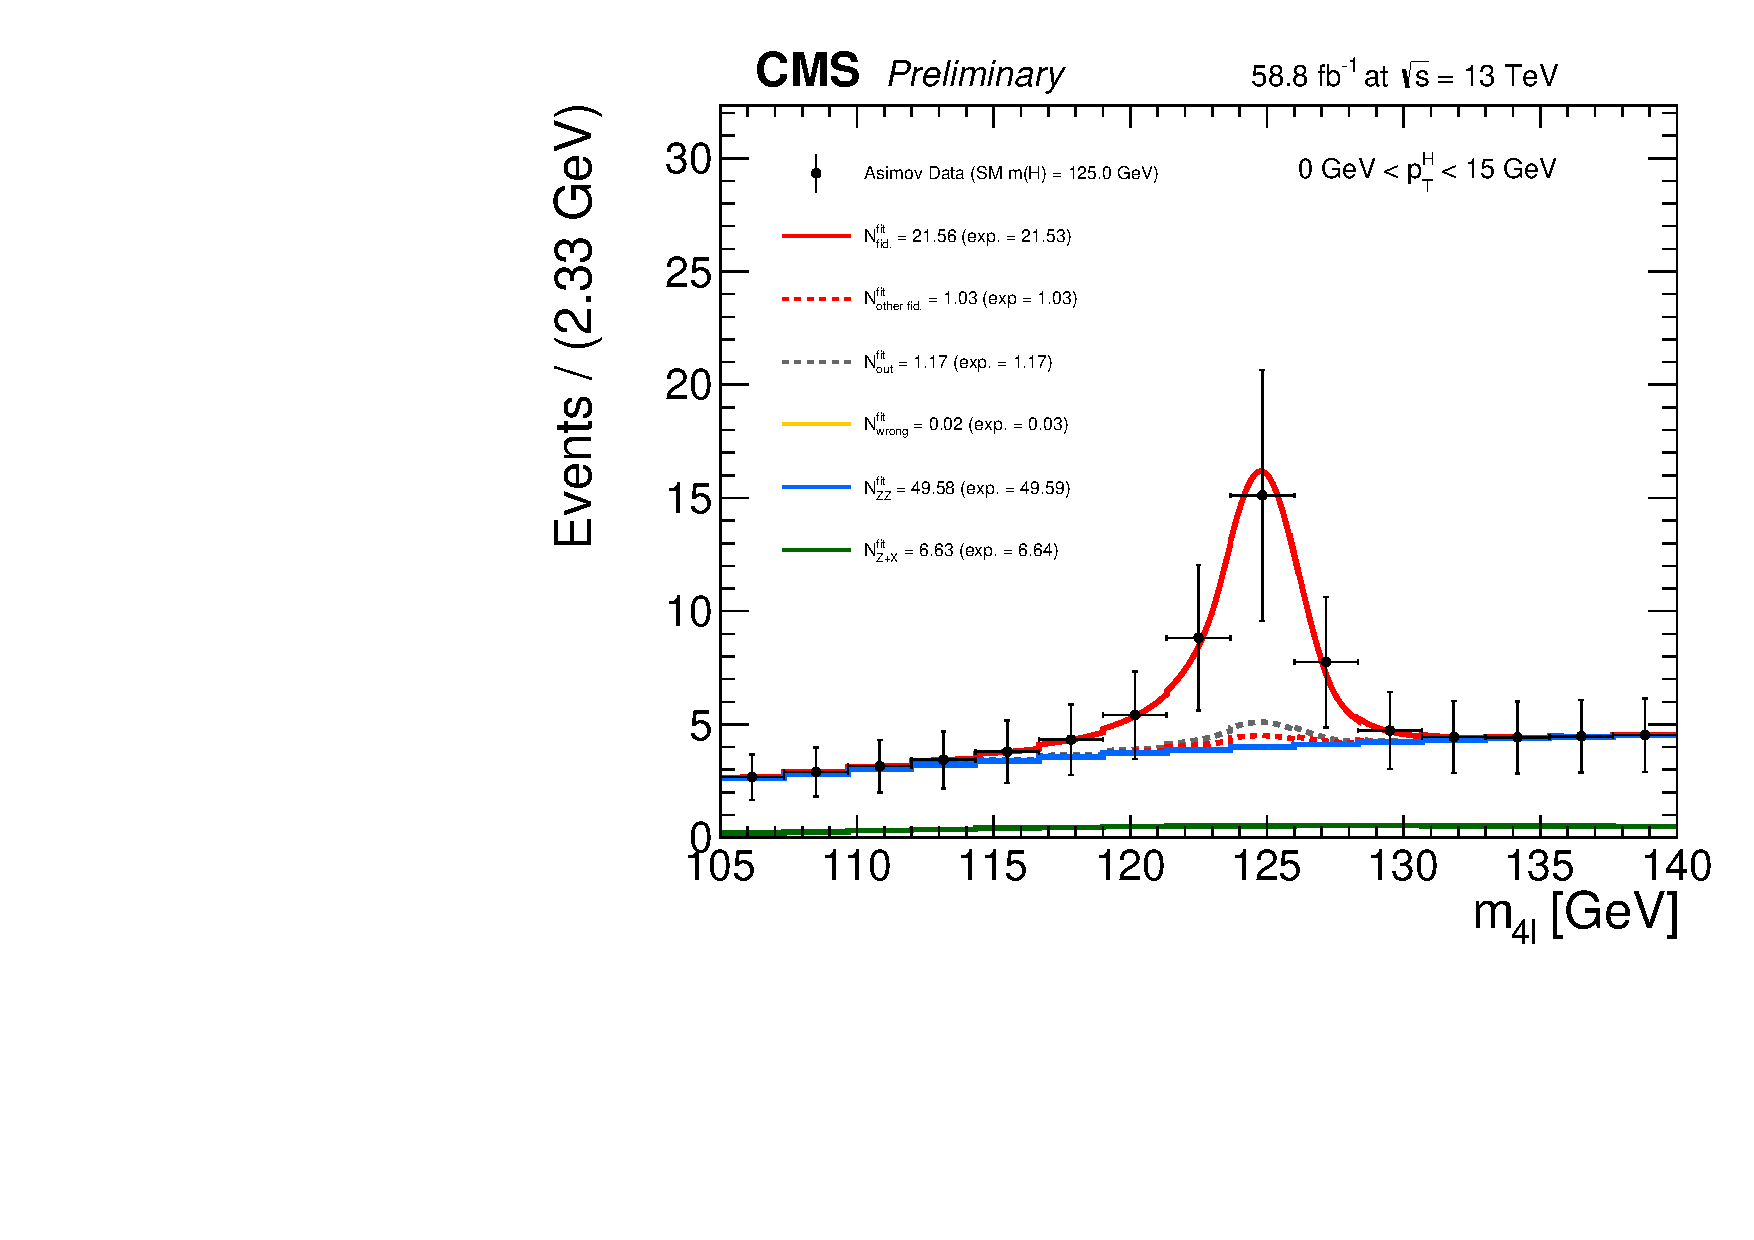
\includegraphics[width=0.40\textwidth,angle=0]{Figures/results/fiducial/2018//asimovdata_SM_125_v2_unfoldwith_SM_125_v3_pT4l_4l_recobin0.pdf}
       \label{fig:sigfits-asimov-SM-pT4l-4l:a}
    }
    \subfigure[$15.0 \GeV < \pt(\mathrm{H}) < 30.0 \GeV$]{
      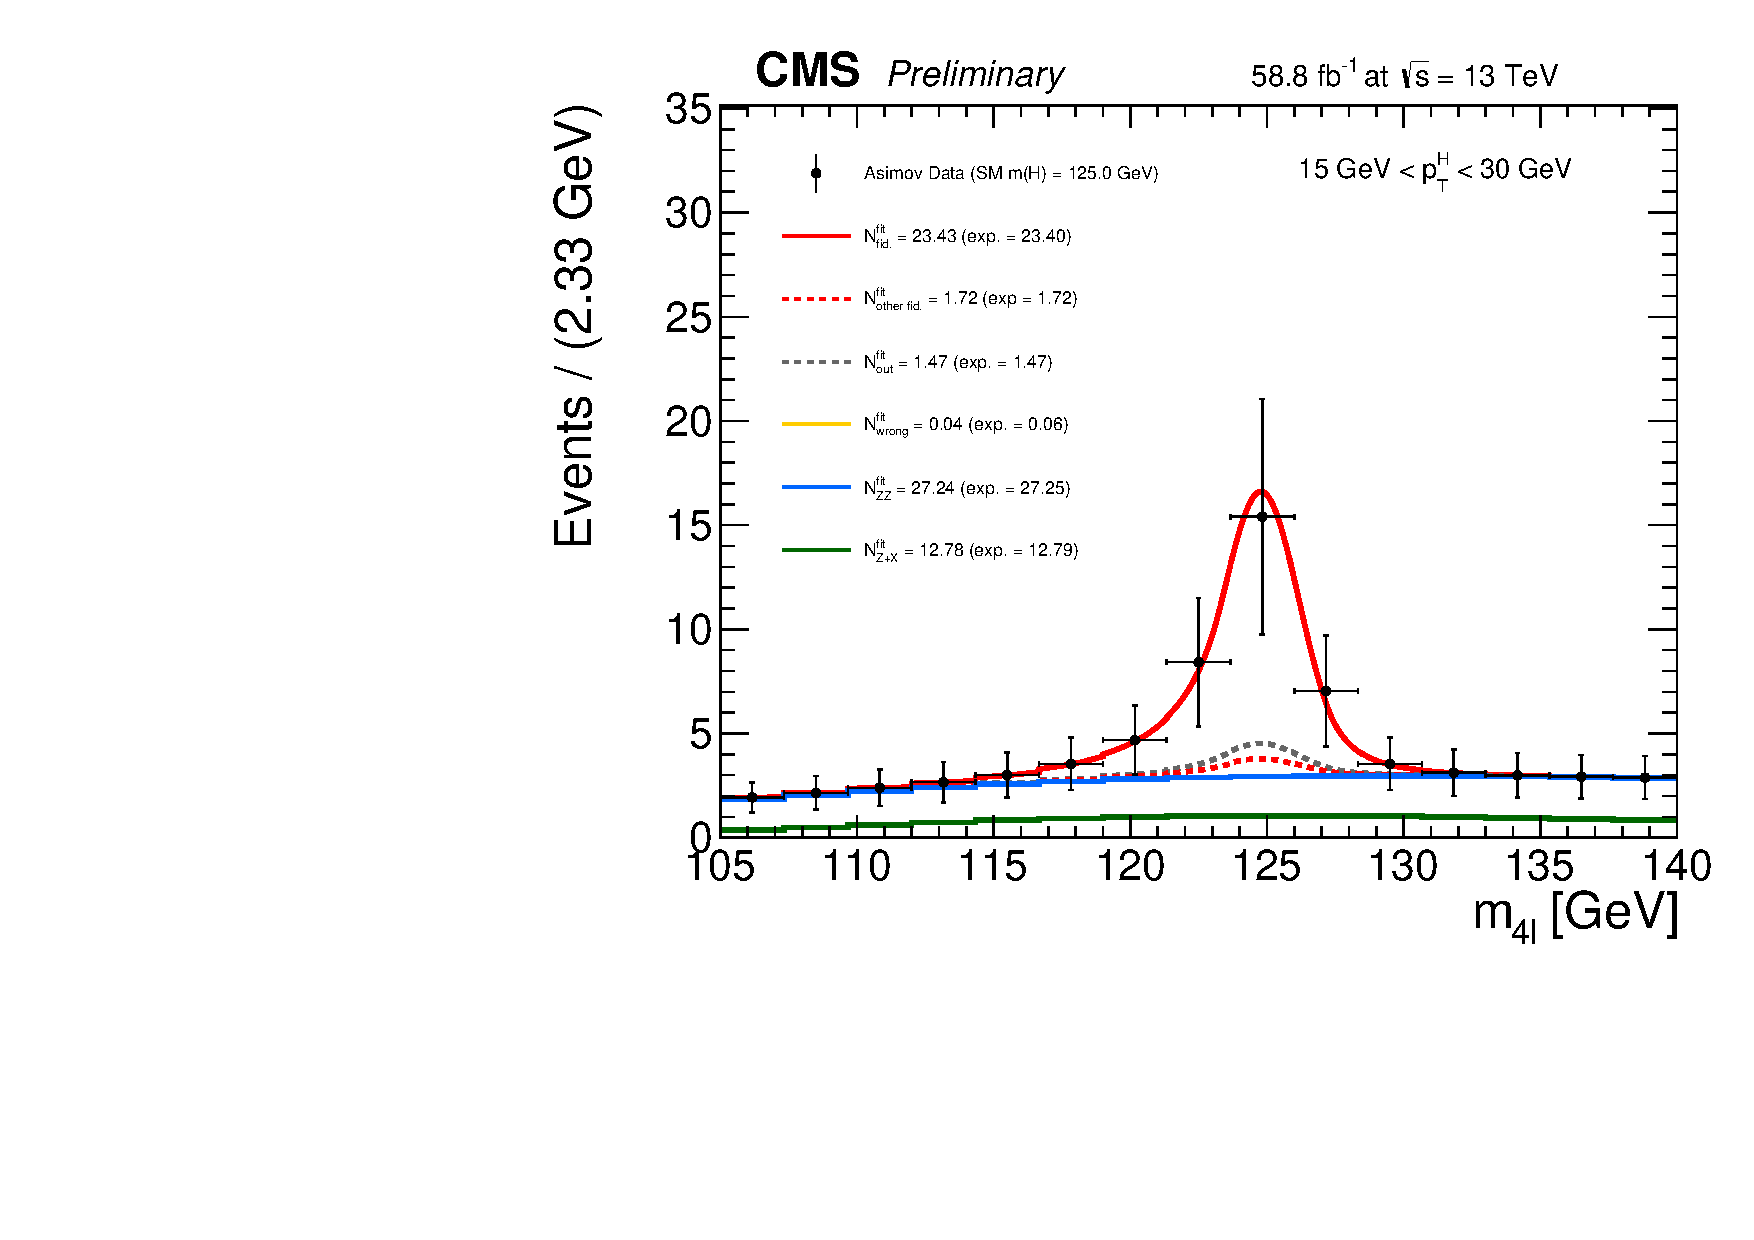
\includegraphics[width=0.40\textwidth,angle=0]{Figures/results/fiducial/2018//asimovdata_SM_125_v2_unfoldwith_SM_125_v3_pT4l_4l_recobin1.pdf}
       \label{fig:sigfits-asimov-SM-pT4l-4l:b}
    } \\
    \subfigure[$30.0 \GeV < \pt(\mathrm{H}) < 45.0 \GeV$]{
      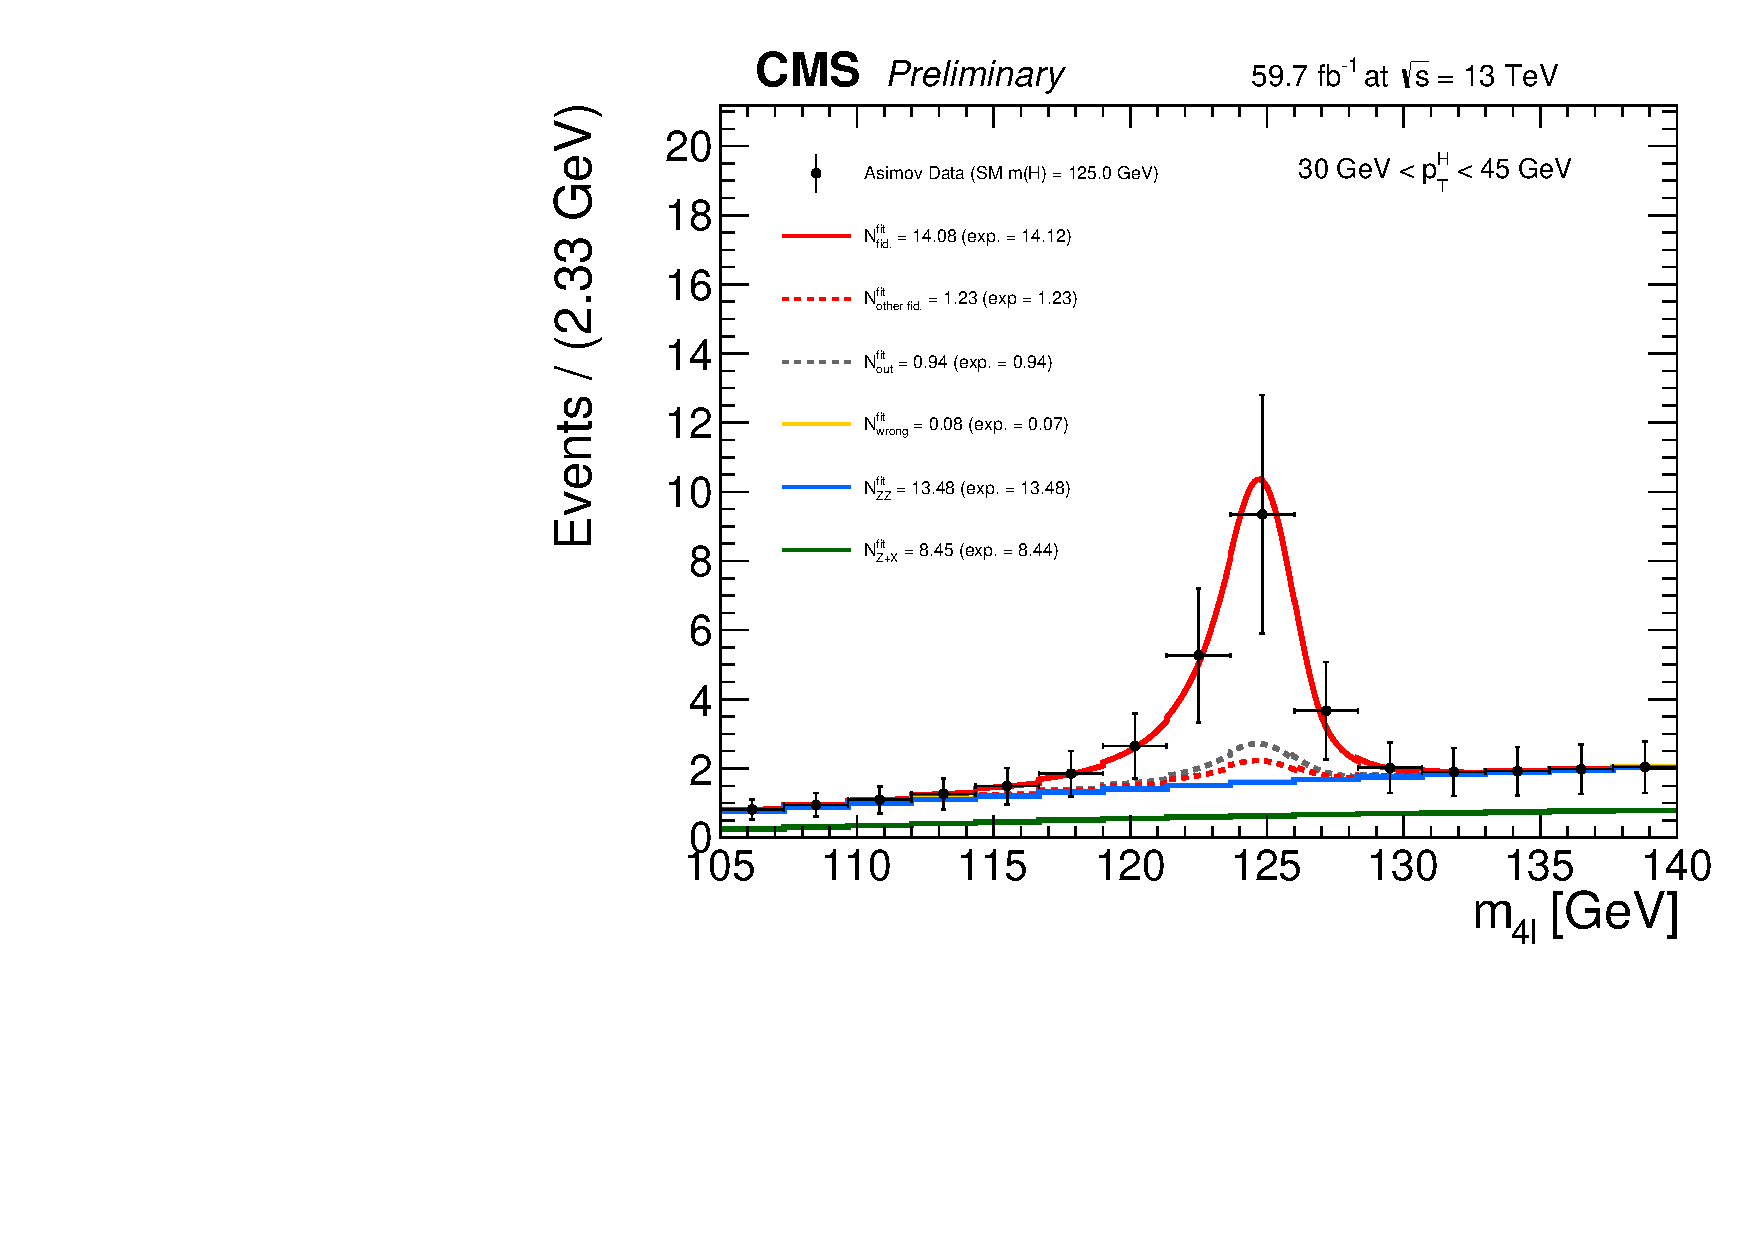
\includegraphics[width=0.40\textwidth,angle=0]{Figures/results/fiducial/2018//asimovdata_SM_125_v2_unfoldwith_SM_125_v3_pT4l_4l_recobin2.pdf}
       \label{fig:sigfits-asimov-SM-pT4l-4l:c}
    }
    \subfigure[$45.0 \GeV < \pt(\mathrm{H}) < 80.0 \GeV$]{
      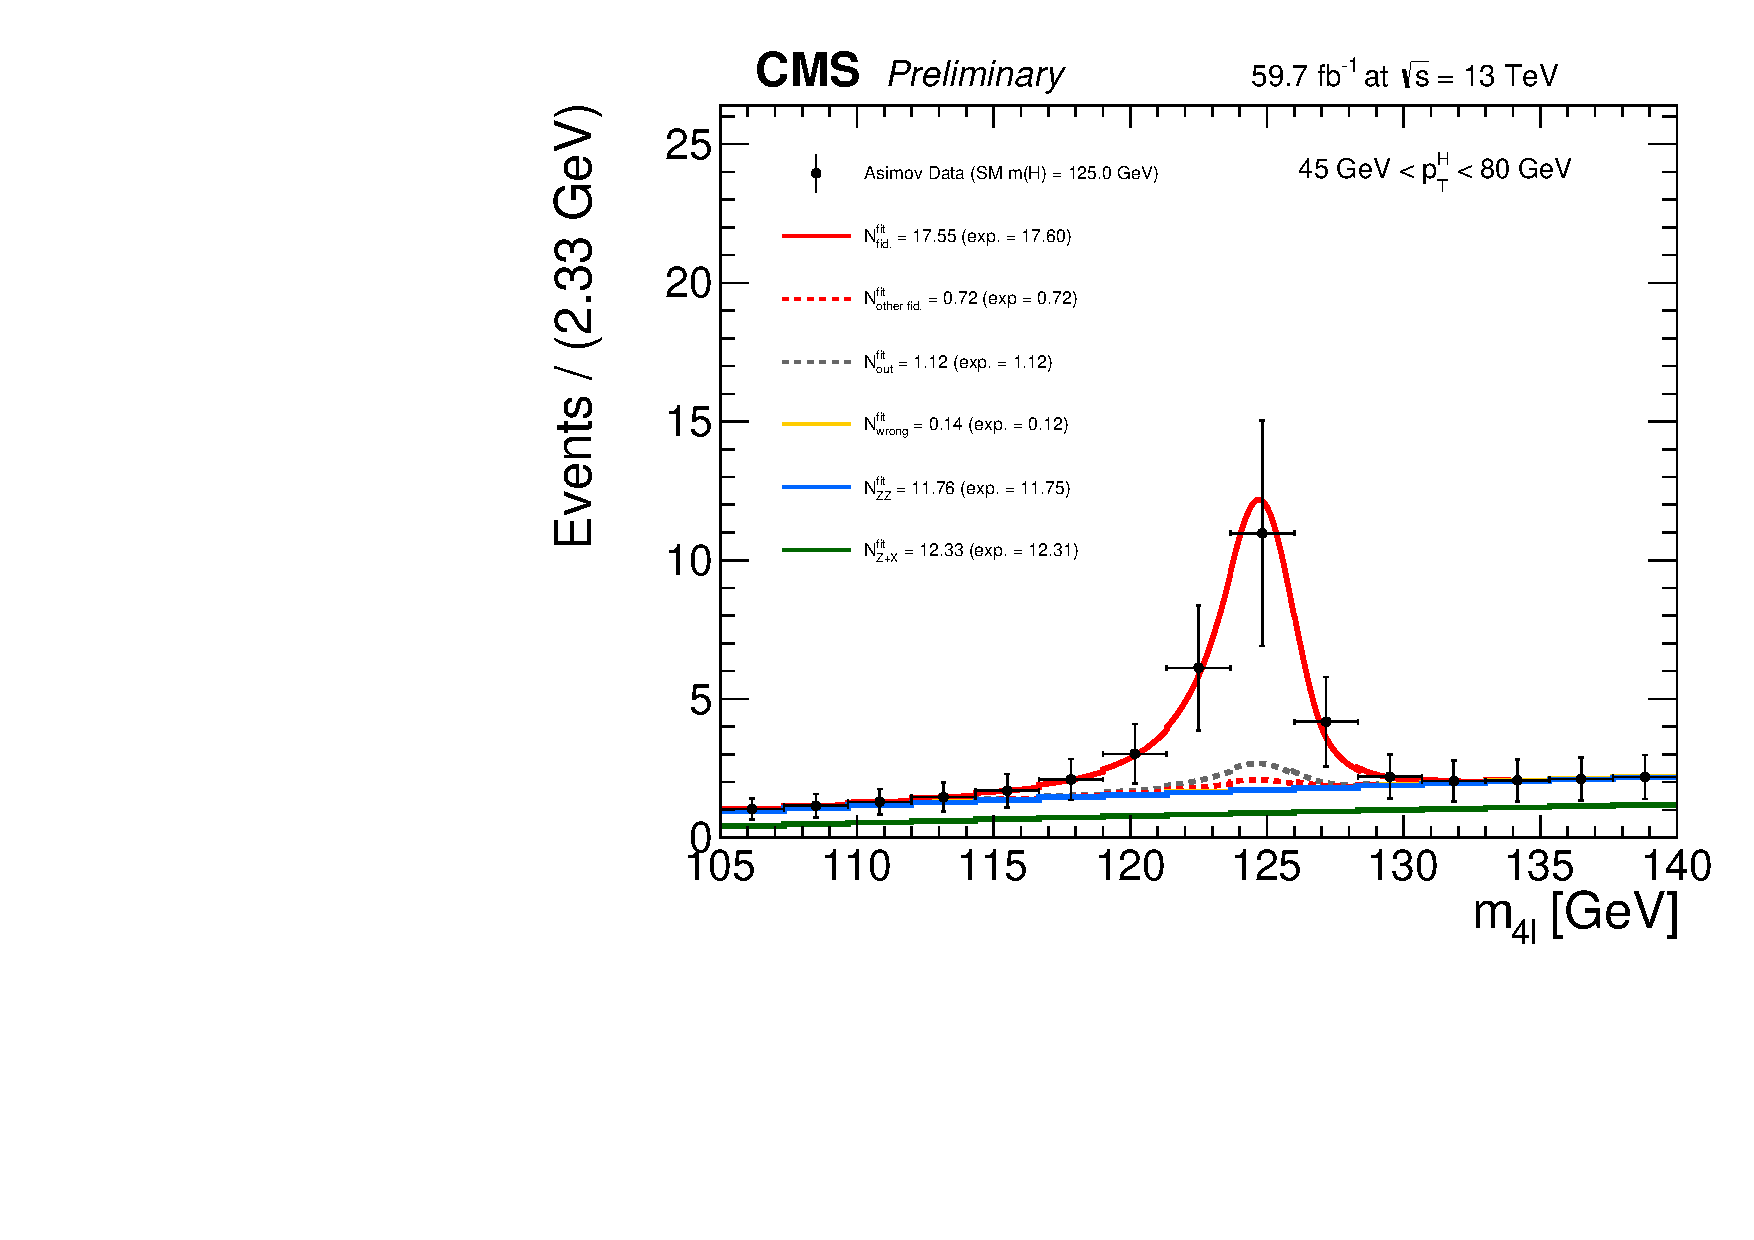
\includegraphics[width=0.40\textwidth,angle=0]{Figures/results/fiducial/2018//asimovdata_SM_125_v2_unfoldwith_SM_125_v3_pT4l_4l_recobin3.pdf}
       \label{fig:sigfits-asimov-SM-pT4l-4l:d}
    } \\
   \subfigure[$80.0 \GeV < \pt(\mathrm{H}) < 120.0 \GeV$]{
      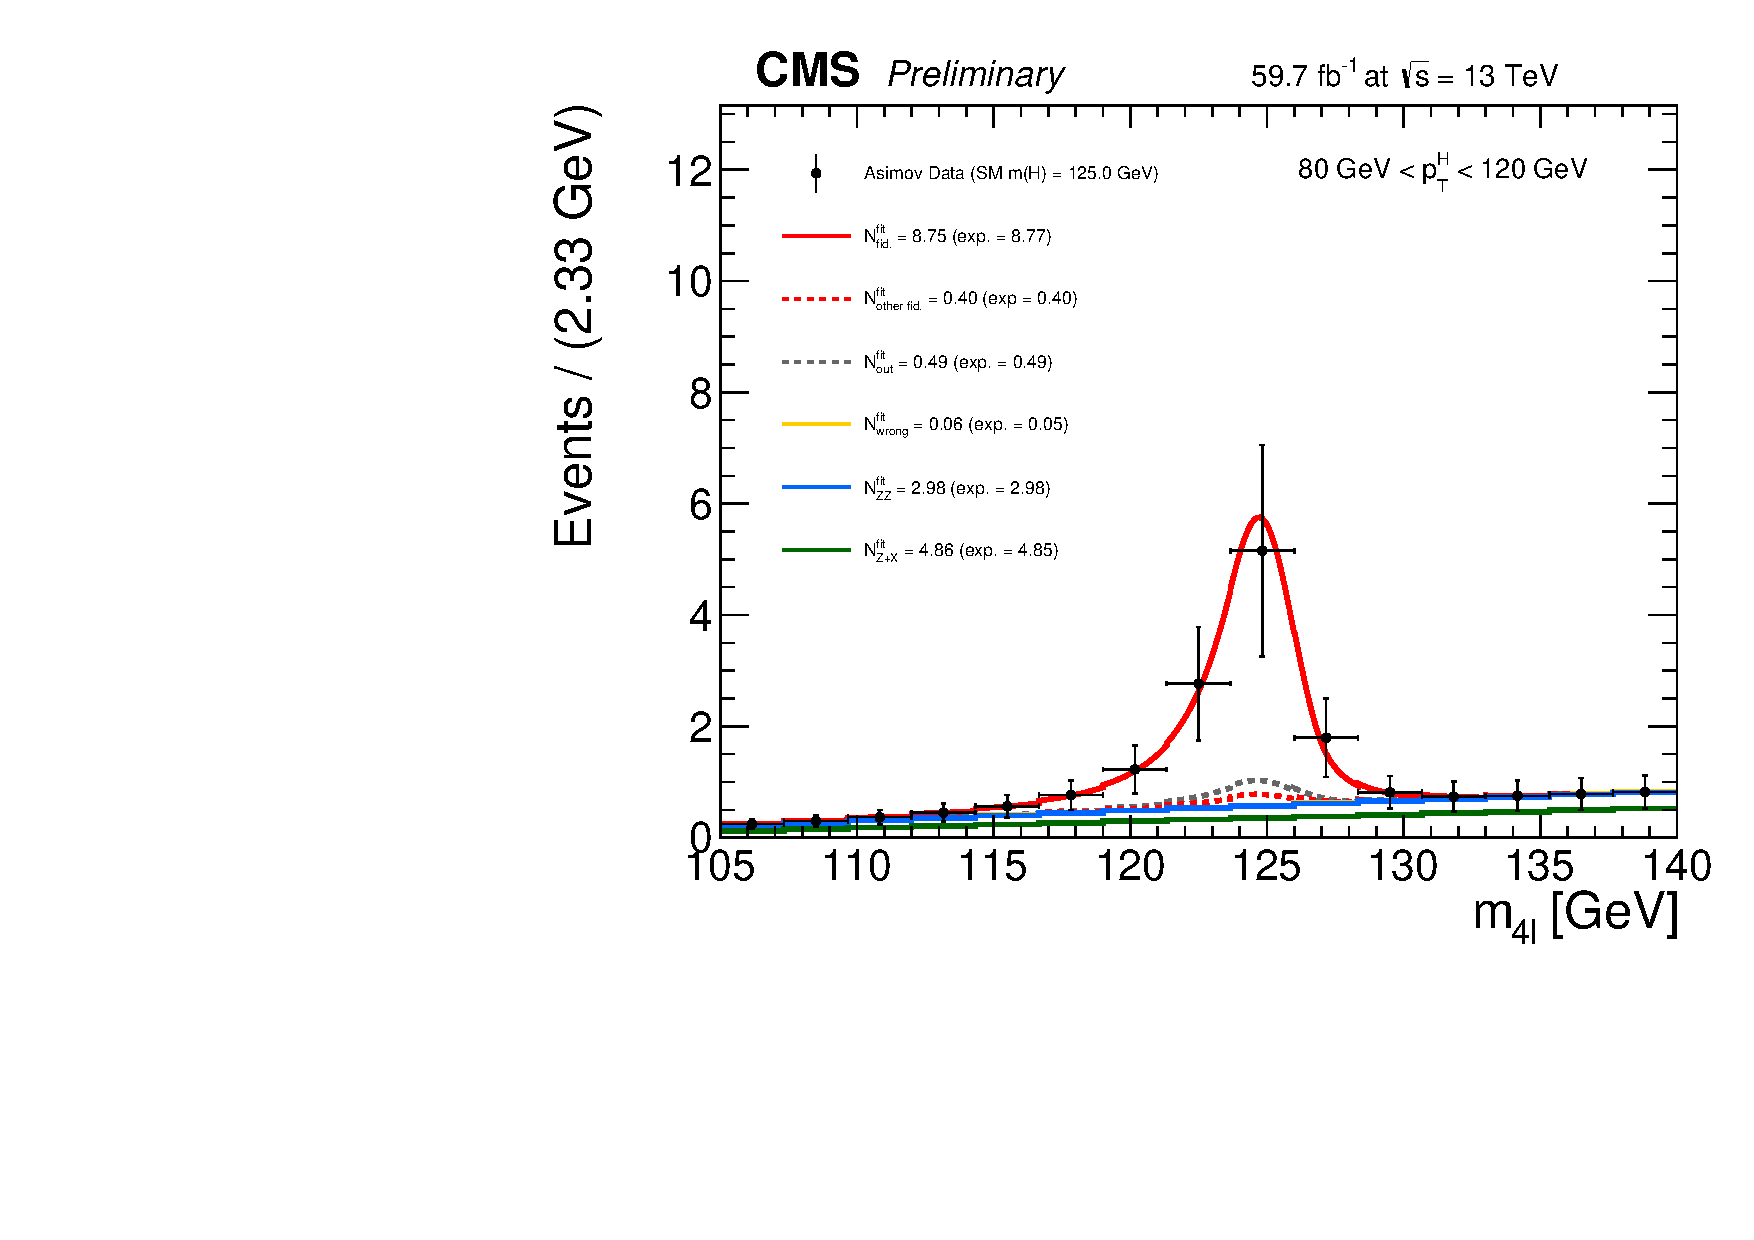
\includegraphics[width=0.40\textwidth,angle=0]{Figures/results/fiducial/2018//asimovdata_SM_125_v2_unfoldwith_SM_125_v3_pT4l_4l_recobin4.pdf}
       \label{fig:sigfits-asimov-SM-pT4l-4l:b}
    } 
    \subfigure[$120.0 \GeV < \pt(\mathrm{H}) < 200.0 \GeV$]{
      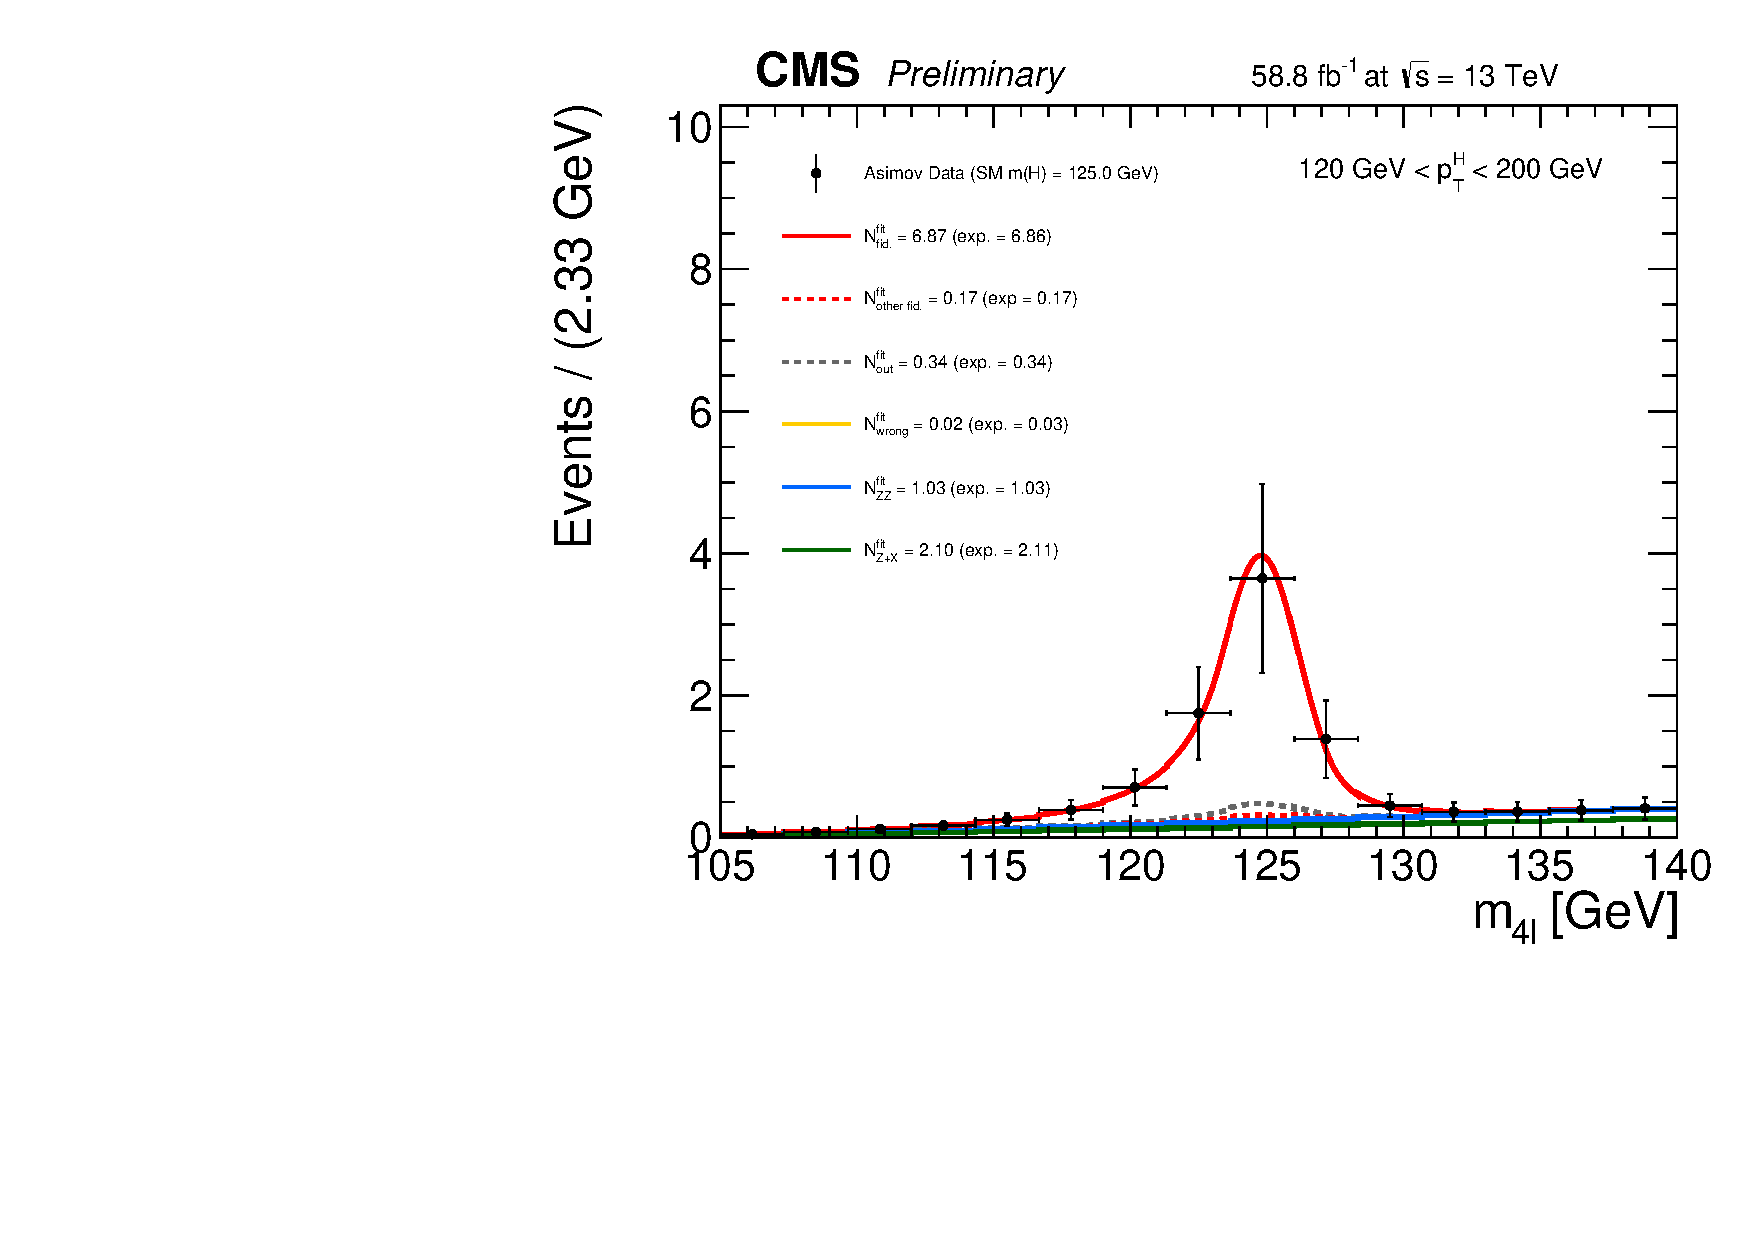
\includegraphics[width=0.40\textwidth,angle=0]{Figures/results/fiducial/2018//asimovdata_SM_125_v2_unfoldwith_SM_125_v3_pT4l_4l_recobin5.pdf}
       \label{fig:sigfits-asimov-SM-pT4l-4l:c}
    } \\  
    \subfigure[$200.0 \GeV < \pt(\mathrm{H}) < 13000.0 \GeV$]{
      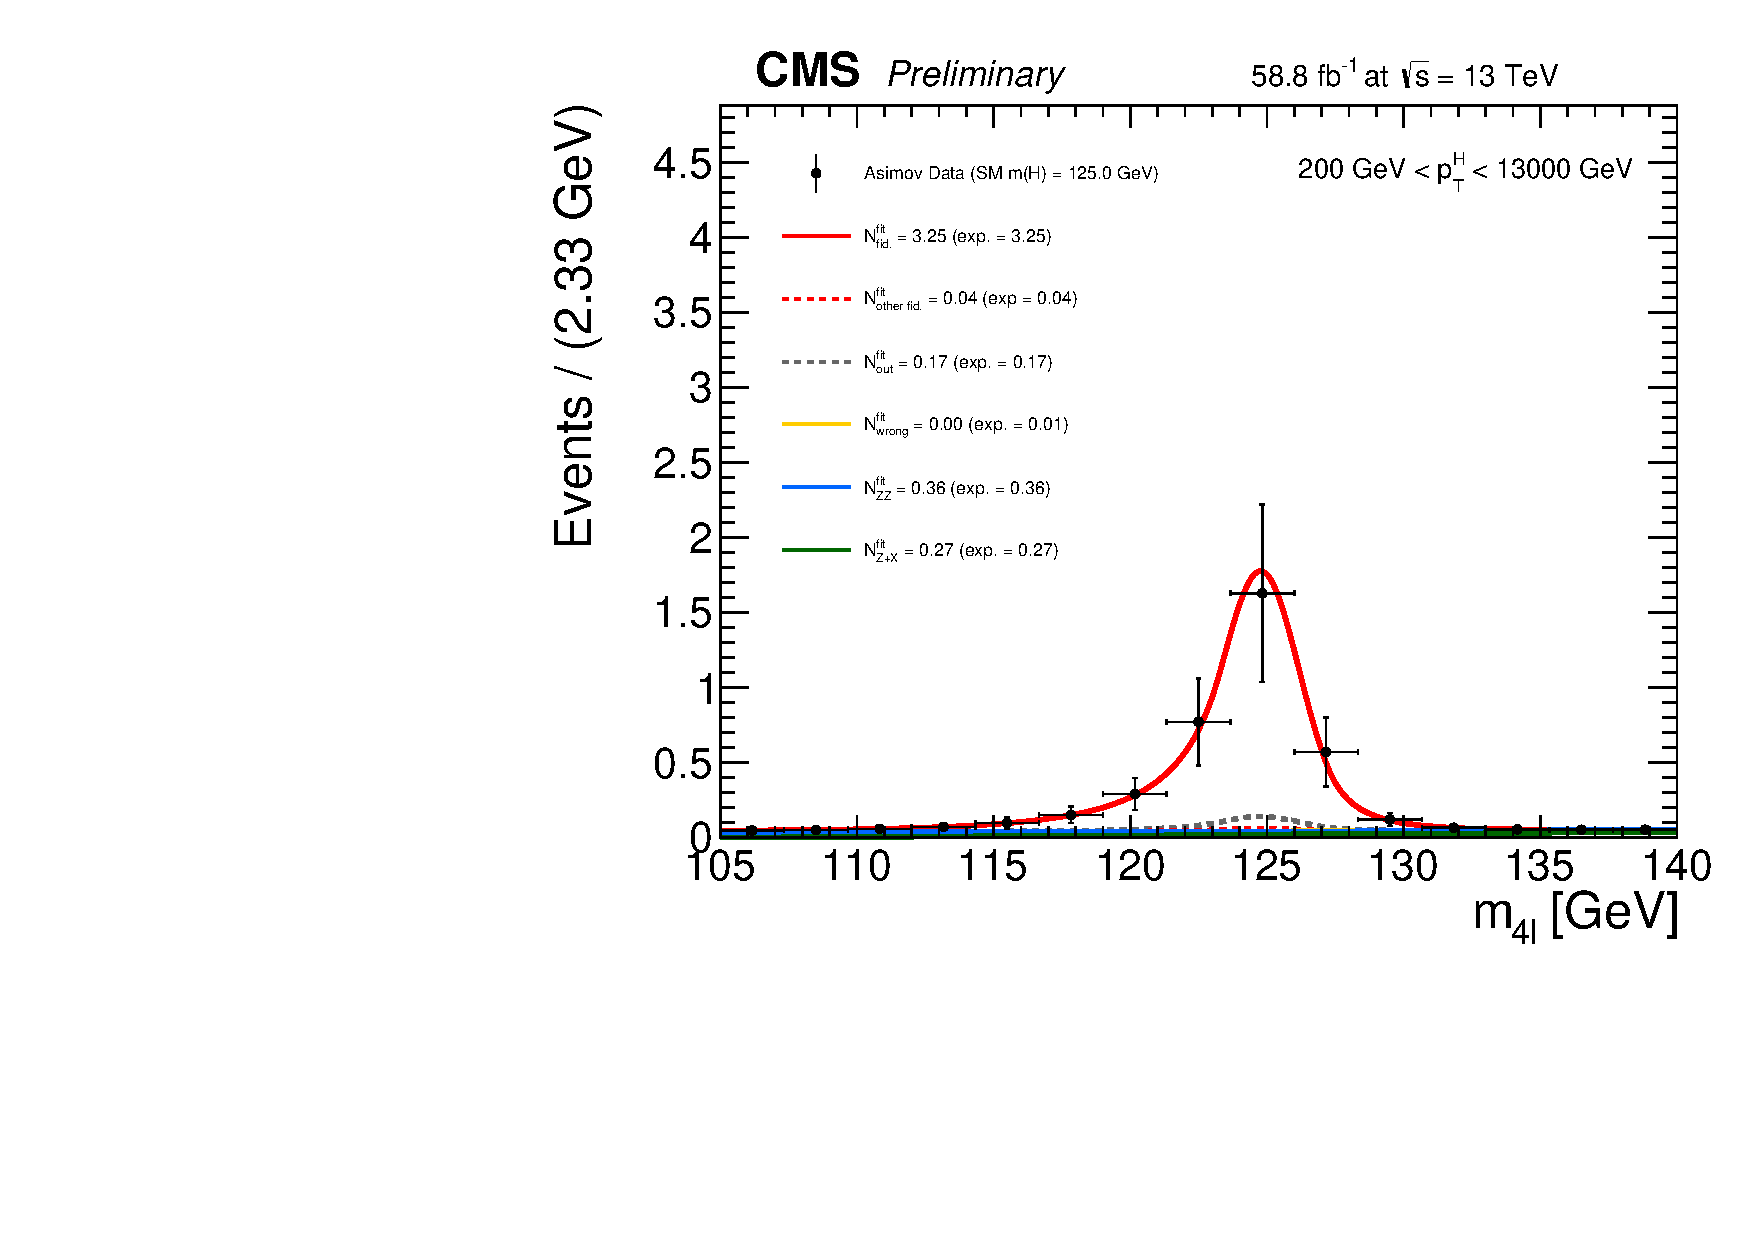
\includegraphics[width=0.40\textwidth,angle=0]{Figures/results/fiducial/2018//asimovdata_SM_125_v2_unfoldwith_SM_125_v3_pT4l_4l_recobin6.pdf}
       \label{fig:sigfits-asimov-SM-pT4l-4l:d}
    } \\
	  
	  \caption{Four lepton mass distributions for an Asimov dataset generated using SM cross section values and SM efficiencies where the gg$\rightarrow$H prediction
    is from {\sc powheg+JHUgen} and resulting fitted values of PDFs of signal and background for different bins of $\pt(\mathrm{H})$ (all final states combined).}
  \label{fig:sigfits-asimov-SM-pt4l-4l}
  \end{center}
\end{figure}

%\clearpage
